\documentclass[a4paper,12pt,oneside]{report}
\usepackage{graphicx}
\usepackage[T1]{fontenc}
\usepackage[utf8]{inputenc}
\usepackage[english]{babel}
\usepackage{fancyhdr}
\usepackage[style=authoryear,minnames = 1, maxbibnames=99, maxcitenames=2,uniquelist=false,uniquename=false,doi=false,url=false,isbn=false, date=year]{biblatex}
\usepackage{xcolor}
\setlength\bibitemsep{1.5\itemsep}
\usepackage[tocindent=4em]{tocloft}
\setlength{\cftfignumwidth}{3em}
\setlength\cftbeforechapskip{10pt}
\renewcommand\cftfigafterpnum{\vskip5pt\par}
\renewcommand\cfttabafterpnum{\vskip5pt\par}


\usepackage{helvet}
\renewcommand{\familydefault}{\sfdefault}


% amsmath and amssymb packages, useful for mathematical formulas and symbols
\usepackage{amsmath,amssymb}

% textcomp package and marvosym package for additional characters
\usepackage{textcomp,marvosym}



\usepackage[acronym, nonumberlist]{glossaries}
\makeglossaries

\newacronym{rgc}{RGC}{retinal ganglion cell}

\newacronym{sc}{SC}{superior colliculus}

\newacronym{lgn}{LGN}{lateral geniculate nucleus}

\newacronym{v1}{V1}{primary visual cortex}


\newacronym{od}{OD}{ocular dominance }
 
\newacronym{md}{MD}{monocular deprivation}

\newacronym{ttx}{TTX}{tetrodotoxin}

\newacronym{nmda}{NMDAR}{ N-methyl-D-aspartate}

\newacronym{ko}{KO}{knockout}

\newacronym{cko}{cKO}{conditional knockout}

\newacronym{wt}{WT}{wild type}

\newacronym{dpf}{dpf}{days post-fertilisation}

\newacronym{stdp}{STDP}{spike timing dependent plasticity}

\newacronym{ampa}{AMPA}{amino-3-hydroxy-5-methyl-4-isoxazolepropionic acid}

\newacronym{ltp}{LTP}{long term potentiation}

\newacronym{ltd}{LTD}{long term depression}

\newacronym{ee}{EE}{environmental enrichment}

\newacronym{pca}{PCA}{Principle Component Analysis}

\newacronym{bina}{BINA}{Bayesian inference of neural assemblies}

\newacronym{hmm}{HMM}{Hidden Markov Model}

\newacronym{li}{LI}{Lateralisation Index}

\newacronym{mi}{MI}{Matching Index}

\newacronym{nr}{NR}{normally reared}

\newacronym{gr}{GR}{gravel reared}

\newacronym{wb}{WB}{white background}

\newacronym{gb}{GB}{gravel background}

\newacronym{anova}{ANOVA}{Analysis of Variance}

\newacronym{dko}{DKO}{double knock out}

\newacronym{dlc}{DLC}{DeepLabCut}

\newacronym{lda}{LDA}{Linear Discriminant Analysis}

\newacronym{logreg}{LogReg}{Logistic Regression}

\newacronym{grin}{\textit{grin2a}}{\textit{grin2aa/ab}}

\newacronym{sem}{SEM}{Standard Error of the Mean}

\newacronym{iprgc}{ipRGC}{intrinsically photosensitive retinal ganglion cell}

\newacronym{onl}{ONL}{outer nuclear layer}

\newacronym{inl}{INL}{inner nuclear layer}

\newacronym{gcl}{GCL}{ganglion cell layer}

\newacronym{ipl}{IPL}{inner plexiform layer}

\newacronym{opl}{OPL}{outer plexiform layer}

\newacronym{cnn}{CNN}{convolutional neural network}

\newacronym{spv}{SPV}{stratum pervienticular}

\newacronym{omr}{OMR}{optomotor response}

\newacronym{okr}{OKR}{optokinetic response}

\newacronym{ncc}{NCC}{neuron correlation coefficient}

\newacronym{hpf}{HPF}{hours post-fertilization}

\newacronym{sd}{SD}{standard deviation}

\newacronym{camkii}{CaMKII}{calmodulin-dependent protein kinase}

\newacronym{talen}{TALEN}{transcription activator-like effector nuclease}

\newacronym{pcr}{PCR}{polymerase chain reaction}




\usepackage{caption}
% the following format will be used to emulate the captions produced by fltpage
\DeclareCaptionLabelFormat{adja-page}{\hrulefill\\#1 #2 \emph{(previous page)}}

\captionsetup{font=footnotesize}

% cite package, to clean up citations in the main text. Do not remove.
%\usepackage{cite}

% Use nameref to cite supporting information files (see Supporting Information section for more info)
%\usepackage{nameref,hyperref}

% line numbers
%\usepackage[right]{lineno}

\setcounter{tocdepth}{2}

\addbibresource{references.bib}

\setlength\parindent{0pt}
\parskip 0.5 cm 
\usepackage[a4paper,width=150mm,left = 20mm,right = 20mm, top=25mm,bottom=25mm,bindingoffset=10mm]{geometry}

\usepackage{setspace} 
\onehalfspacing
 
\graphicspath{{Figures/}} 
 


%\title{
  %  {\center{}{The effect of environmental enrichment on tectal dynamics and tectally-mediated behaviour}} \\
   % {\newline \large{King's College London}} \\
    % \\
%}

%\author{Thomas T. J. Sainsbury}












\begin{document}
    \addcontentsline{toc}{chapter}{Title page}
    \begin{titlepage}
   \begin{center}
       \vspace*{1cm}
    
       \LARGE
       \textbf{The effect of environmental enrichment on tectal dynamics and tectally-mediated behaviour}
            
       \vspace{1.5cm}
        \large
       \textbf{Thomas T. J Sainsbury}
       
       \vspace{1cm}
       
       \text{Supervisors:} 
       \vspace{0.1cm}
       
       \text{Dr. Martin Meyer (primary supervisor)}
       \vspace{1cm}
       \text{Prof. Robert Hindges (secondary supervisor)}

       \vfill
            
       A thesis presented for the degree of\\
       Doctor of Philosophy
            
       \vspace{0.8cm}

            
       Centre for Developmental Neurobiology\\
       Institute of Psychiatry, Psychology \& Neuroscience\\
       King's College London\\
            
   \end{center}
\end{titlepage}
    
    
    
    
    \chapter*{Abstract}
    \addcontentsline{toc}{chapter}{Abstract}
    Different visual environments can present unique challenges for the visual system. Even individuals of the same species can occupy very distinct ecological niches. To ensure that the performance of visually-guided behaviours is maintained in the face of environmental diversity, the development of visual systems is plastic, enabling adaptive changes according to environmental demands. 

    A wealth of experimental evidence demonstrates that visual experience during developmental periods can alter both the structure and function of individual neurons, the organization of sensory maps and even the number of neurons in the brain. However, in most cases it is not known if or how these changes modify behaviour. Furthermore, because behaviour is an emergent property of activity in distributed populations of neurons, it is challenging to relate changes in the properties of individual neurons and maps to behaviour.  To address this, I have used larval zebrafish as a model to determine how enrichment of the visual environment (raising fish on a bed of gravel) impacts the structure and dynamics of population activity in the visual system and the performance of visually-guided behaviour. 
    
    Using 2-photon volumetric imaging to capture the activity of thousands of neurons throughout the optic tectum of the larval zebrafish (the largest visual area of the zebrafish brain) combined with Bayesian inference techniques I have shown that environmental enrichment has a profound effect on the dynamics and developmental trajectory of spontaneous tectal assemblies. Furthermore, I show using a prey-capture assay that hunting performance of larval zebrafish raised in enriched and non-enriched environments is equal if the assay is performed against a non-textured background. However, zebrafish raised in the enriched environment consume significantly more prey than larvae raised in a non-enriched environment when larvae from both groups hunt in visual background containing gravel. These results suggest that environmental enrichment modifies the structure of population activity in the tectum and that this correlates with improved performance of a tectally-mediated behaviour in a complex visual environment. 
    
    To understand which forms of plasticity may be underlying these experience dependent changes we generated zebrafish carrying null mutations in \textit{grin2aa} and \textit{grin2ab} which code for isoforms of the NR2A subunit of the NMDA receptor. I find that the effects of environmental enrichment are blocked in \textit{grin2aa/ab} double mutants, suggesting that the subunit composition of the NMDAR is crucial for mediating the effects of environmental enrichment on functional development of the tectum. 
    
    Finally, changes in behaviour are difficult to relate to changes in spontaneous tectal activity. Therefore I developed a "virtual reality" hunting assay that allows for neural activity in the tectum and tail movements to be recorded whilst the larvae are presented with stimuli that resemble prey. To mimic the hunting assay these stimuli are presented over textured and non-textured backgrounds and the position of the stimulus was decoded from tectal activity. Preliminary results suggest that tectal representation of prey location may be contextually modulated by the background with decoding performance increasing when the stimuli were viewed over the textured background. This setup will allow for differences between gravel reared and normally reared fish in visually evoked tectal activity to be investigated in future experiments.
  
      
      
    \clearpage
    \chapter*{Acknowledgements}
    \addcontentsline{toc}{chapter}{Acknowledgements}
     This thesis has been one of the most enjoyable and rewarding experiences that I have undertaken in my life. Whilst, at times, undertaking a PhD can feel a bit like a roller-coaster and present major challenges I have been lucky enough to have a large number of extremely supportive individuals around me. Without these people (and others!) this PhD would not have come to fruition.
 
 Firstly, I would like to express my sincerest gratitude to Dr Martin Meyer for supervising me on this project with tireless patience, dedication and mentoring. He has always given me freedom to dream and conduct new experiments whilst grounding me and keeping me on course. Above all, his excitement and enthusiasm towards new data and new questions is what has constantly inspired me and pushed me forward with this project. I could not have wished for a better supervisor. Besides my supervisor, I would like to thank my second supervisor Dr. Robert Hindges and my thesis committee members Dr. Juan Burrone and Dr. Isaac Bianco for their insightful comments and contributions.
 
 Thank you to all of the Meyer lab past and present: Dom, Dylan, Jade, Kostas, Nikolas, Matt, Paul, Rachel, Richard and Tom R. Working with all of you over these past few years has been a pleasure. You have all made the lab an enjoyable place to work and each one of you has contributed to the way I think as a scientist today. Special mentions go to both Giovanni Diana and Thomas Shallcross. Giovanni, I cannot describe how much I have learnt from you these past few years. You have changed the way that I think about and approach problems whilst becoming a friend for life. You have been an integral part of this project and I feel that the final results chapter was a chance for me to put into action many of the things that I have learnt from you. Tom, thank you for your support as a house mate and as a colleague. Our science chats in the pub and your support have helped me immensely.
 
 I would also like to thank friends from the CDN and beyond for your help and support over the years: Hannah, Suzie, Andy, Simon, Elin, Samir, Athena and many others.
 
 Last but not least I would like to show my sincerest gratitude to Alina, Mum, Dad, Alice, Gwil and Sophie. I have been a wreck these past few months, I would not have got through it without you. From the bottom of my heart thank you.
 
    
    \clearpage
    \tableofcontents
    \addcontentsline{toc}{chapter}{Table of contents}
    \clearpage
    \listoffigures
    \addcontentsline{toc}{chapter}{List of figures}
    
    
    \clearpage
    
    \printglossary[type=\acronymtype,title=Abbreviations,nonumberlist]
    %
\newacronym{rgc}{RGC}{retinal ganglion cell}

\newacronym{sc}{SC}{superior colliculus}

\newacronym{lgn}{LGN}{lateral geniculate nucleus}

\newacronym{v1}{V1}{primary visual cortex}


\newacronym{od}{OD}{ocular dominance }
 
\newacronym{md}{MD}{monocular deprivation}

\newacronym{ttx}{TTX}{tetrodotoxin}

\newacronym{nmda}{NMDAR}{ N-methyl-D-aspartate}

\newacronym{ko}{KO}{knockout}

\newacronym{cko}{cKO}{conditional knockout}

\newacronym{wt}{WT}{wild type}

\newacronym{dpf}{dpf}{days post-fertilisation}

\newacronym{stdp}{STDP}{spike timing dependent plasticity}

\newacronym{ampa}{AMPA}{amino-3-hydroxy-5-methyl-4-isoxazolepropionic acid}

\newacronym{ltp}{LTP}{long term potentiation}

\newacronym{ltd}{LTD}{long term depression}

\newacronym{ee}{EE}{environmental enrichment}

\newacronym{pca}{PCA}{Principle Component Analysis}

\newacronym{bina}{BINA}{Bayesian inference of neural assemblies}

\newacronym{hmm}{HMM}{Hidden Markov Model}

\newacronym{li}{LI}{Lateralisation Index}

\newacronym{mi}{MI}{Matching Index}

\newacronym{nr}{NR}{normally reared}

\newacronym{gr}{GR}{gravel reared}

\newacronym{wb}{WB}{white background}

\newacronym{gb}{GB}{gravel background}

\newacronym{anova}{ANOVA}{Analysis of Variance}

\newacronym{dko}{DKO}{double knock out}

\newacronym{dlc}{DLC}{DeepLabCut}

\newacronym{lda}{LDA}{Linear Discriminant Analysis}

\newacronym{logreg}{LogReg}{Logistic Regression}

\newacronym{grin}{\textit{grin2a}}{\textit{grin2aa/ab}}

\newacronym{sem}{SEM}{Standard Error of the Mean}

\newacronym{iprgc}{ipRGC}{intrinsically photosensitive retinal ganglion cell}

\newacronym{onl}{ONL}{outer nuclear layer}

\newacronym{inl}{INL}{inner nuclear layer}

\newacronym{gcl}{GCL}{ganglion cell layer}

\newacronym{ipl}{IPL}{inner plexiform layer}

\newacronym{opl}{OPL}{outer plexiform layer}

\newacronym{cnn}{CNN}{convolutional neural network}

\newacronym{spv}{SPV}{stratum pervienticular}

\newacronym{omr}{OMR}{optomotor response}

\newacronym{okr}{OKR}{optokinetic response}

\newacronym{ncc}{NCC}{neuron correlation coefficient}

\newacronym{hpf}{HPF}{hours post-fertilization}

\newacronym{sd}{SD}{standard deviation}

\newacronym{camkii}{CaMKII}{calmodulin-dependent protein kinase}

\newacronym{talen}{TALEN}{transcription activator-like effector nuclease}

\newacronym{pcr}{PCR}{polymerase chain reaction}

    \addcontentsline{toc}{chapter}{Abbreviations}
    
    \chapter{Introduction}
    A fundamental goal of neuroscience is to understand how precise patterns of connectivity between neurons arise and how, once formed, they underlie mental processes, such as perception, cognition and behaviour. Although many areas of the nervous system have been analysed with this goal in mind, the visual system has been particularly well studied. A number of features of the visual system make it an excellent model for studying brain development. One is that, as highly visual animals, humans have an intuitive understanding of what the visual system does. We can therefore more readily design stimuli to probe visual system capabilities, perhaps more so than other areas of the brain, such as the motor or other sensory systems. Vision is the neural process which converts light into a rich array of electrical signals which are distributed across large populations of neurons. The brain uses this activity to generate visual percepts, creating internal representations of the location and qualities of visual features in the environment. These features are then used to drive visual behaviours. Despite this, our understanding of how circuits form in the visual system is far from complete. We know even less about how properties of circuit development may contribute to changes in visual perception and visually driven behaviour. However, what is now universally accepted is that both genetic programs, activity- and experience-dependent mechanisms work in unison to construct the visual system. The goal of this thesis is to use zebrafish larvae to understand how natural features in the visual scene contribute to the formation of visually guided behaviour, and also how these features affect the organisation of population activity during development.

This chapter will give an overview of the visual system and the fundamental mechanisms that shape its development. Particular emphasis will be devoted to the studies that have shown how activity, often driven by visual experience, shapes the formation of sensory maps, neuronal morphology and the functional properties of neurons. This chapter will furthermore explain how these studies have typically used artificial manipulations of the visual scene, have been limited by methodology to studying coarse anatomy or single neurons and have not investigated the impact of these changes on visually guided behaviour. More recently, the ability to record  neural activity from large populations of neurons alongside behaviour has rapidly increased, enabling the relationship between developing population activity and behaviour to examined.  These techniques can be combined with naturalistic manipulations of the visual scene through \gls{ee} to investigate the role of different types of visual experience on visual system development. This chapter will conclude with a brief introduction of the larval zebrafish and describe the properties of this system that make it a powerful model for studying developing neural circuits and behaviour. 

\section{Development of the visual system and the role of visual experience}

\subsection{The visual pathway: from retina to brain}
In vertebrates, vision begins in the retina, a well conserved multi-laminated structure containing well defined cell types. These cells are organised into three nuclear layers: the \gls{onl}, the \gls{inl} and the \gls{gcl}. Sitting between these, are two neuropil layers where synaptic transmission takes place. These are known as the \gls{opl} and  \gls{ipl} (\textbf{Figure \ref{fig:i_ret}A}). Through this organisation, the cells in the retina transform the spatiotemporal pattern of light into neural responses which encode specific features of the visual scene (\cite{Masland2012TheRetina}).

First, incoming light is focused by the lens creating an image on the retina. Light sensitive photoreceptors sitting in the ONL (rod and cones), transduce this incoming light into electrical signals via the activation of opsins.  These opsins are G-protein coupled receptors which absorb photons at specific wavelengths of light, triggering hyperpolarization of the photoreceptor (\cite{Palczewski2006GRhodopsin}). This leads to a reduction in synaptic glutamate release onto the dendrites of bipolar cells in the OPL . Bipolar cells can either maintain this signal (OFF) or invert it (ON) such that OFF-bipolar cells are hyperpolarised by light and ON-bipolar cells are depolarised (\cite{Werblin1969OrganizationRecording.}; \cite{Masu1995SpecificGene}).  The axons of bipolar cells synapse in different strata of the IPL. OFF-bipolar cells synapse in the outer IPL (OFF strata) whereas ON-bipolar cells synapse in the inner IPL (ON strata) (\cite{Euler2014RetinalVision}). It is within these strata that bipolar cells pass on visual information to \glspl{rgc}. RGCs have their cell bodies in the GCL and act as the output cells of the retina. In addition to these cell types, there are two main classes of interneuron in the retina: horizontal cells and amacrine cells which modulate information as it is transferred across the retina (\cite{Masland2012TheRetina, Hoon2014FunctionalDisease}). This modulation serves to refine and filter the visual scene to shape the “receptive field” properties of RGCs. As a result, they serve as detectors for certain visual features at particular points in space.


The types of information that are encoded by RGCs have been found to be extremely diverse with over 30 different functional subtypes being identified in mice (\cite{Sanes2015TheClassification}; \cite{Baden2016TheMouse}). In the simplest case, many RGCs have been shown to respond to either increases in luminance (ON-RGCs), decreases in luminance (OFF-RGCs) or both (ON-OFF-RGCs) (\cite{Hartline1938TheRetina, Lettvin1959WhatBrain, Barlow1953}). However, RGCs can encode more precise visual features such as specific directions of motion (\cite{BARLOW1963, Oyster1967,Lettvin1959WhatBrain}), and the orientation of edges (\cite{Levick1967ReceptiveRetina}; \cite{Maturana1963DirectionalRetina}). Furthermore, there are also RGCs tuned to very complex features including “bug detectors” in frogs (\cite{Barlow1953, Lettvin1959WhatBrain}), local motion detectors in mice (\cite{Zhang2012}) and prey and predator detectors in zebrafish (\cite{Semmelhack2014}; \cite{Temizer2015}). Together these RGCs create multiple parallel output channels from the retina, carrying feature specific information to the brain.

To reach the brain RGC axons must leave the eye through the optic nerve. They then distribute this information to multiple different regions of the brain, ranging from 10 retinociepient areas in zebrafish (\cite{Robles2014}) to over 40 in mammals (\cite{Morin2014RetinofugalMouse}) (\textbf{Figure \ref{fig:i_ret}B}). Studies examining the projection patterns of individual RGC subtypes have shown each of these areas receives input from unique combinations of RGCs (\cite{Robles2014}; \cite{Dhande2014RetinalProcessing}). These regions can then use this information to generate different visuomotor behaviours. 

For some retinorecipient areas of the brain RGC input is relatively simple and the relationship to behaviour is well defined. For example, some RGCs are intrinsically photosensitive  (\acrshort{iprgc}s) due to their expression of the photopigment melatonin causing them to  fire in response to ambient light levels (\cite{Hattar2002Melanopsin-containingPhotosensitivity, Berson2002PhototransductionClock}). ipRGCs have been found to project to both the suprachiasmatic nucleus and olivary pretectal nucleus where their activity is used to regulate circadian rhythms and the pupillary light reflex, respectively (\cite{Pickard1985BifurcatingThalamus, Hattar2006CentralMouse, Guler2008MelanopsinVision, Chen2011PhotoentrainmentIpRGCs}). Similarly, the accessory optic system in the pretectum receives input from different subtypes of direction selective RGCs (\cite{Simpson1984TheSystem, Hoffmann1991FunctionalMonkeys, Brodsky2012TheStrabismus}). Each of these subtypes projects to different pretectal nuclei. Here this information is used to drive the \gls{okr}, a reflexive movement of the eyes that maintains gaze in response movement of the head, or rotational whole field motion (\cite{Dhande2014RetinalProcessing}; \cite{Distler2011VisualMonkeys}). 

For other regions of the brain \gls{rgc} input is more complex and is processed further to drive diverse sets of different behaviours. In fish, frogs and chicks, the main retinorecipient is the optic tectum which is equivalent to the \gls{sc} in mammals (\cite{Goodhill2005}).  The SC/optic tectum receives input from multiple different RGC subtypes, integrates it with different sensory modalities and  generates new receptive field properties (\cite{Robles2014}; \cite{Dhande2014RetinalProcessing}; \cite{Hunter2013}). This information is used to guide movement relative to specific locations in egocentric space (\cite{Gandhi2011MotorColliculus}). This can include shifting the movement of the eyes to particular locations in visual space, orienting movements of the body and reaching movements in primates (\cite{Straschill1970ActivityMovements,Sparks1976SizeColliculus, Stuphorn2000NeuronsCoordinates, Song2015NeuralColliculus}). Furthermore, in fish and frogs, it generates coordinated eye and body movements to bring about complex behaviours such as prey capture or predator avoidance (\cite{Gahtan2005, Bianco2015, Dunn2016,Ewert1987NeuroethologyToads,King1996VisuallyCapture}). 

In mammals, the principle retinorecipient target is the \gls{lgn} within the thalamus. While the LGN does receive small contributions from feature selective RGC, the majority of RGC input is relatively simple, encoding changes in luminance at particular points in visual space (\cite{Jeffries2014MappingMethods}; \cite{Kim2008MolecularMotion}).  From the LGN, this visual information is then relayed to the \gls{v1} by thalamocortical projections. At sequential stages within the visual cortex more complex visual features are generated, starting with orientation selective cells (\cite{Hubel1962ReceptiveCortex}), building up to more complex receptive fields (\cite{Martinez2001ConstructionCortex}).

\begin{figure}[!ht]
        \center{\includegraphics[width =  0.7\paperwidth]{Figures/retina_schematic.jpg}}
            \caption[\textbf{\label{fig:i_ret}\textbf{Cellular organisation of the retina and its targets.}}]{ \textbf{\label{fig:i_ret} Cellular organisation of the retina and its targets.} \textbf{(A)}  A schematic of the vertebrate visual system showing the organisation of the retina. The names of cell types, cellular layers and synaptic layers are reported. RGCs project to multiple regions of the brain including the superior colliculus (called optic tectum in lower vertebrates). In mammals RGCs also project to the visual cortex via the LGN. Image is from (\cite{Sanes2010DesignSystems}). \textbf{(B)} A 3D reconstruction of RGCs (grey) targeting multiple retinorecipient recipient regions of the brain. In fish there are 10 RGC retinorecipient areas called abourisation fields (AF1-10), the optic tectum is AF 10. Each arborisation field receives unique combinations of RGC subtypes. Image is from (\cite{Robles2014}).}
      \end{figure}

\subsection{Molecular cues guide axons to their targets.}
For the visual system to perform its function RGCs first need to be guided to their target regions and find their synaptic targets. Then within those regions precise connectivity needs to be established creating neural circuits that are capable of generating visually guided behaviours. Such circuitry is shaped by a combination of intrinsic and extrinsic factors.

In early visual system development, the axons of RGCs leave the retina, bundle together in the optic tract, and target retinorecipient regions of the brain. For many retinorecipient areas, this targeting of axons occurs in a manner that maintains the relative positions of the RGC somata in the retina, preserving a map of visual space in the target region (\cite{Luo2007DevelopmentMaps., Huberman2008MechanismsFields}). Such retinotopic maps are widespread in the visual system but perhaps one of the best studied is that of the optic tectum (\cite{Goodhill2005}). In fish and frogs, developing RGC axons exiting the eye fully decussate, targeting the contralateral tectum.  Axons originating in the nasal retina project to the anterior tectum and those stemming from the temporal retina terminate in the posterior tectum (\cite{Attardi1963PreferentialFibers}). Similarly, the dorso-ventral axis of the retina is transformed along the medio-lateral axis of the tectum. This preservation of the visual map in tectal coordinates requires relatively precise targeting of axons guided by molecular cues. The first evidence for this came from an elegant experiment by Sperry (\citeyear{Sperry1963CHEMOAFFINITYPATTERNS}) who was studying the regenerating retino-tectal pathway of frogs. In these experiments, the optic nerve was sectioned, the eye was rotated 180 degrees, and reattached so that the axons could regenerate. Sperry found that, despite this perturbation, regenerating RGC axons grew back to the same termination site, maintaining the same topographic order that they had previously held. This resulted in a reversed map of visual space and caused the frogs behaviour to be directed in the opposite direction to visual stimuli (\cite{Sperry1943EffectCoordination, Sperry1963CHEMOAFFINITYPATTERNS}) (\textbf{Figure \ref{fig:I_frog_sperry}}). This prompted the “chemoaffinity” hypothesis, in which the molecular tagging of axons and their targets acts as  “postal code”, guiding them to their termination site (Sperry 1963). Under this model, growing axon could be extended, retracted, or turned by regions of the target tissue expressing either attractive or repulsive cues (\cite{Meyer1998RogerHypothesis}). Further evidence for this model came from growing chick RGCs over stripes of tectal tissue in \textit{ex vivo} preparations. These demonstrated that RGCs from the temporal retina were repelled by stripes of posterior tectum and that this effect could be abolished through high temperature treatments that denatured proteins in the tectal substrate (\cite{Walter1987RecognitionVitro}).

\begin{figure}[!ht]
        \center{\includegraphics[width =  0.7\paperwidth]{Figures/I_frog_sperry.jpg}}
            \caption[\textbf{\label{fig:I_frog_sperry}\textbf{Sperry’s chemoaffinity hypothesis.}}]{\textbf{\label{fig:I_frog_sperry}Sperry’s chemoaffinity hypothesis.} Frogs are able to direct their behaviour towards their prey. RGCs positioned in the nasal retinal target anterior tectum (Ant.) whereas those with their somatas in temporal retina target the posterior tectum (Post.). Rotating the frog’s eye 180 degrees causes them to move in the opposite direction relative to visual stimuli. This is because the regenerating RGCs grow back to their original position within the tectum, resulting in a reversed map of visual space. For clarity the dorsal ventral axis have not been shown but these are also reversed.}
      \end{figure}

It is now known that numerous molecular cues are expressed within both the retina and tectum in complementary gradients. These exert a combined influence in positioning axon terminals within the tectum and many cues are well conserved across species (\cite{McLaughlin2003RetinotopicDevelopment, Feldheim2010VisualCompetition., Higenell2012ExpressionLaevis}). A large number of these identified cues belong to the ephrin family (\cite{Egea2007BidirectionalGuidance, Drescher1997TheGuidance}). Ephrins are membrane bound ligands which are expressed as a gradient within the tectum whereas their binding partners, the Eph receptors, are expressed by RGCs in gradients across the retina. The most well studied members of this family are EphrinA-EphA interactions, which allow for the temporal-nasal axis of the retina to be mapped to the anterior-posterior axis of the tectum (\cite{Triplett2012EphMaps}). This is because Ephrin-A is expressed in decreasing concentrations from the posterior to the anterior tectum (\cite{Drescher1995InKinases, Brennan1997TwoZebrafish, Higenell2012ExpressionLaevis, McLaughlin2003RetinotopicDevelopment}). This gradient repels Eph-A expressing RGCs from temporal retina, shifting their termination zone anteriorly (\cite{Drescher1997TheGuidance}). Blocking this pathway either through EphA knockout or pharmacological inhibition results in a disordered retinotectal map with axons overshooting their typical termination site (\cite{Woo2009RetinotopicAdhesion, Sweeney2015Ephrin-asTypes}). Similarly, the dorsoventral axis of the retina is thought to be mapped to the mediolateral tectum by EphB-EphrinB signalling and semaphorin3D, a molecule that repels ventral RGCs expressing neurophilin 1A/1D (\cite{Hindges2002EphBMapping., Brennan1997TwoZebrafish, Liu2012}). In addition to these, many more molecular cues have been identified in zebrafish through large scale mutagenesis followed by screening for retinotopic mapping defects (\cite{Baier1996GeneticProjection, Karlstrom1996ZebrafishPathfinding}). Together these studies show that numerous molecules are important for establishing retinotopic maps in the developing retinotectal system.

The action of molecular cues is not restricted to specifying retinotopy, and early work in chick showed that the laminar organisation of the tectum is also specified by molecular cues. For example, an extracellular protein, Nel, has been found to divert some RGC axons away from specific lamina (\cite{Jiang2009InNel}). In fish, a similar mechanism causes RGCs expressing the Robo2 receptor to target different regions of a superficial-to-deep gradient of Slit1 within the tectum (\cite{Xiao2011AssemblyCollagen}). This was thought to be significant because each of these lamina contain the terminal axons of RGCs that are tuned to stimuli moving in different directions. This suggests that molecular cues may be important for specifying cell-type-specific connections, potentially facilitating genetically predetermined tectal computations. However, this view was challenged by an experiment in a zebrafish line, known as the \textit{astray} mutant, which is a functional null for the Robo-2 receptor (\cite{Campbell2007Slit1aPathways}). While these mutants did show disorganised tectal lamina and deficits in the directional tuning of tectal neurons in early development, no functional deficits were found in later stages of development (\cite{Nikolaou2015LaminationCircuits}). This indicates that the establishment of lamina may be important for accelerating the development of tectal connections rather than cell-type-specific connectivity.

\subsection{Patterned activity propagates through the developing visual system}

Shortly after molecular cues direct developing RGCs to their targets, high levels of patterned neural activity can be found propagating throughout the developing visual system of many species (\cite{Pratt2016AnDevelopment}). There is a wealth of experimental evidence demonstrating that this activity plays a major role in shaping the organisation, connectivity, and physiological properties of sensory systems. A major source of this activity are retinal neurons responding to visual input. Naturalistic visual scenes contain changes in luminance and colour that are spatiotemporally structured. This spatial structure is reflected in the retina by causing neighboring neurons to be correlated in their firing (\cite{Demas2012VisionRetina}). Furthermore, as an organism moves through its environment the position of objects shift over the retina creating optic flow in the temporal to nasal direction, creating patterned activity structured in both space and time  (\cite{Hiramoto2014OpticInformation}). In species which develop externally, termed anamniotic, such as fish and frogs, visual experience can drive patterned activity throughout the visual system as soon as RGCs make their first synaptic connections with their projection targets (\cite{Holt1983OrderFibres}). Therefore visual experience is present at a time when neurons are establishing nascent connections, potentially shaping the refinement of this circuitry.

In contrast, amniotic species spend much of their development devoid of visual stimuli, either behind a thick shell, \textit{in ovo}, or within the womb, \textit{in utero} (\textbf{Figure \ref{fig:I_visual_expeirence_fig}}). Whilst visual stimulation has the potential to pattern the visual system post eye-opening or hatching, early visual system development must occur independently of such visually evoked activity. Nevertheless, in these species, it has been observed that there are high levels of  activity within the retina, which due to its apparent intrinsic generation is often called spontaneous activity. This activity takes the form of waves that travel over the retina and have been observed in multiple species including turtles (\cite{Sernagor1996InfluenceFields}), chicks (\cite{Wong1998DevelopmentallyRetina}), and various mammals (\cite{Meister1991SynchronousRetina, Wong1993TransientRetina, Torborg2005SpontaneousProjections, Ackman2012RetinalSystem, Warland2006DynamicsPathways}). In mammals, retinal waves occur in three stages: type I retinal waves that are driven by gap junctions, type II waves that are caused by starburst amacrine cells through the release of acetylcholine, and type III waves which require glutamate (\cite{Torborg2005SpontaneousProjections, Bansal2000MiceRetina, Kerschensteiner2016GlutamatergicWaves, Syed2004Stage-dependentRetina}). Early work on retinal waves relied on \textit{in vitro} preparations using retinal explants, revealing precise local correlations, reminiscent of those induced by visual stimulation  (\cite{Meister1991SynchronousRetina, Wong1993TransientRetina, Feller1996RequirementWaves}). In more recent work, Ackman et al., (2012) monitored neural activity in the terminals of RGCs in the SC of mice by bulk loading with a fluorescent reporter of activity and optically imaging the fluorescent changes. This revealed two things: firstly, that retinal waves propagate throughout the visual system and, secondly, that these waves are likely to move from temporal to nasal retina. The latter is particularly interesting because this travelling activation resembles activity that would be induced by optic flow in a swimming tadpole or fish, species in which retinal waves are either totally or largely absent (\cite{Kutsarova2017RulesBrain}). This has led to the suggestion that retinal waves exist as an evolutionary adaptation, compensating for the loss of visually evoked activity, made necessary by the transition of amniotic species to land and internal development (\cite{Pratt2016AnDevelopment}). 

Interestingly, despite developing externally, a single type of retinal wave has been identified in zebrafish (\cite{Zhang2016StereotypedAutoreceptors}). These occur very early in development, at a time-point when RGCs are making their initial synapses with tectal neurons, starting around 2.5 \gls{dpf} and finishing around 3 dpf. It is thought that retinal waves in fish may aid visual experience in shaping initial retinotectal connectivity, contributing to their relatively rapid visual system development. 

The literature on the role of activity, whether visually induced or intrinsic, in shaping the visual system is extensive. The following sections will highlight some of the classical experiments which have contributed to our understanding of this process. Particular focus will be devoted to the role of visual experience in shaping sensory maps, neuron morphology, and the functional properties of neurons within the visual system.




\begin{figure}[!ht]
        \center{\includegraphics[width =  0.7\paperwidth]{Figures/I_visual_expeirence_fig.jpg}}
            \caption[\textbf{\label{fig:I_visual_expeirence_fig}\textbf{The extent of visual experience during early visual system development.}}]{ \textbf{\label{fig:I_visual_expeirence_fig}  The extent of visual experience during early visual system development.} \textbf{Left:} Amniotic species during early development are shielded from the visual world by their internal development, viewing total darkness (represented by the black circle). Therefore as neurons in the visual system are making their first synaptic connections they cannot be influenced by the visual environment. Instead they rely on spontaneously driven retinal waves to pattern the visual system. \textbf{Right:} An underwater photo of a natural zebrafish habitat.  As the development of anamniotic embryos takes place externally, they are exposed to visual scenes like this one as neural circuitry is forming. This visual stimulation activates RGCs and thier activity can be used to shape the visual system through activity dependent mechanisms. (Photo courtesy of Tom Baden)}

      \end{figure}

\subsection{Activity shapes the formation of visual maps}
\subsubsection{The formation of ocular dominance columns}
In mammals, outgrowing retinal projections do not fully decussate. Instead, a proportion of RGCs project ipsilaterally with the proportion of ipsilateral projections depending on the species (\cite{Larsson2011BinocularCoordination}). This means the SC, LGN, and visual cortex contain information originating from both eyes which may be important for generating binocular vision. In the cortex, this information is segregated into cortical bands known as \gls{od} columns (\cite{Hubel1969AnatomicalCortex}). Within these columns, cortical neurons show a preference in their responses to stimuli presented to either eye (\cite{Hubel1962ReceptiveCortex}). In a series of experiments, Hubel (\citeyear{Hubel1982Exploration1955-78}) and Wiesel (\citeyear{Wiesel1982PostnatalEnvironment}) showed that the development of this preference was highly dependent on visual experience. In these studies, an eye of a kitten or primate was sutured shut, depriving the eye of visual input (monocular deprivation - \acrshort{md}), and the animal was left to mature to adulthood. Removing the deprivation and performing electrophysiological recordings from single cortical neurons revealed that very few responses could be elicited when visual stimulation was given to the previously deprived eye. Instead, neurons showed a shift in responses towards the open eye, known as an OD shift (\cite{Hubel1970TheKittens, Hubel1977PlasticityCortex., Wiesel1963Single-cellEye, Wiesel1965ComparisonKittens.}). Furthermore, the effects of MD were found to be most pronounced within a particular developmental window in early development because MD outside of this window has little effect in shifting OD.  This suggested that the formation of OD columns could be altered by the lack of visual input, within a defined developmental period, known as the “critical period”, where the brain is in a highly plastic state (\cite{Hubel1970TheKittens}). 

In a second set of experiments Hubel and Wiesel demonstrated that the structure of OD columns were also affected by injecting radiolabeled amino acids into either  eye  in monkeys. This tracer was taken up by the RGCs projecting to the LGN where it transynapsaptically labelled thalamocortical projection neurons. This allowed for their axon terminals to be visualised within the visual cortex. Imaging sections of the visual cortex for autoradiography allowed for visualisation of OD columns as labelled and unlabeled bands (\textbf{Figure \ref{fig:I_sensory_maps}A}). In a monkey whose visual input has not been altered, these bands are of equal sizes, indicating that both eyes are equally represented within the cortex (\cite{Wiesel1974AutoradiographicTransport}). However, MD during development resulted in shrinkage of the OD bands representing the deprived eye (\cite{Hubel1977PlasticityCortex.}). This demonstrated that OD shifts were caused by gross anatomical changes in the regions of the cortex devoted to each eye. Together these observations indicate that there is a competitive mechanism between neurons based on activity, leading to more active afferents expanding their territory, forming more connections with cortical neurons at the expense of less active cells.

\begin{figure}[!ht]
        \center{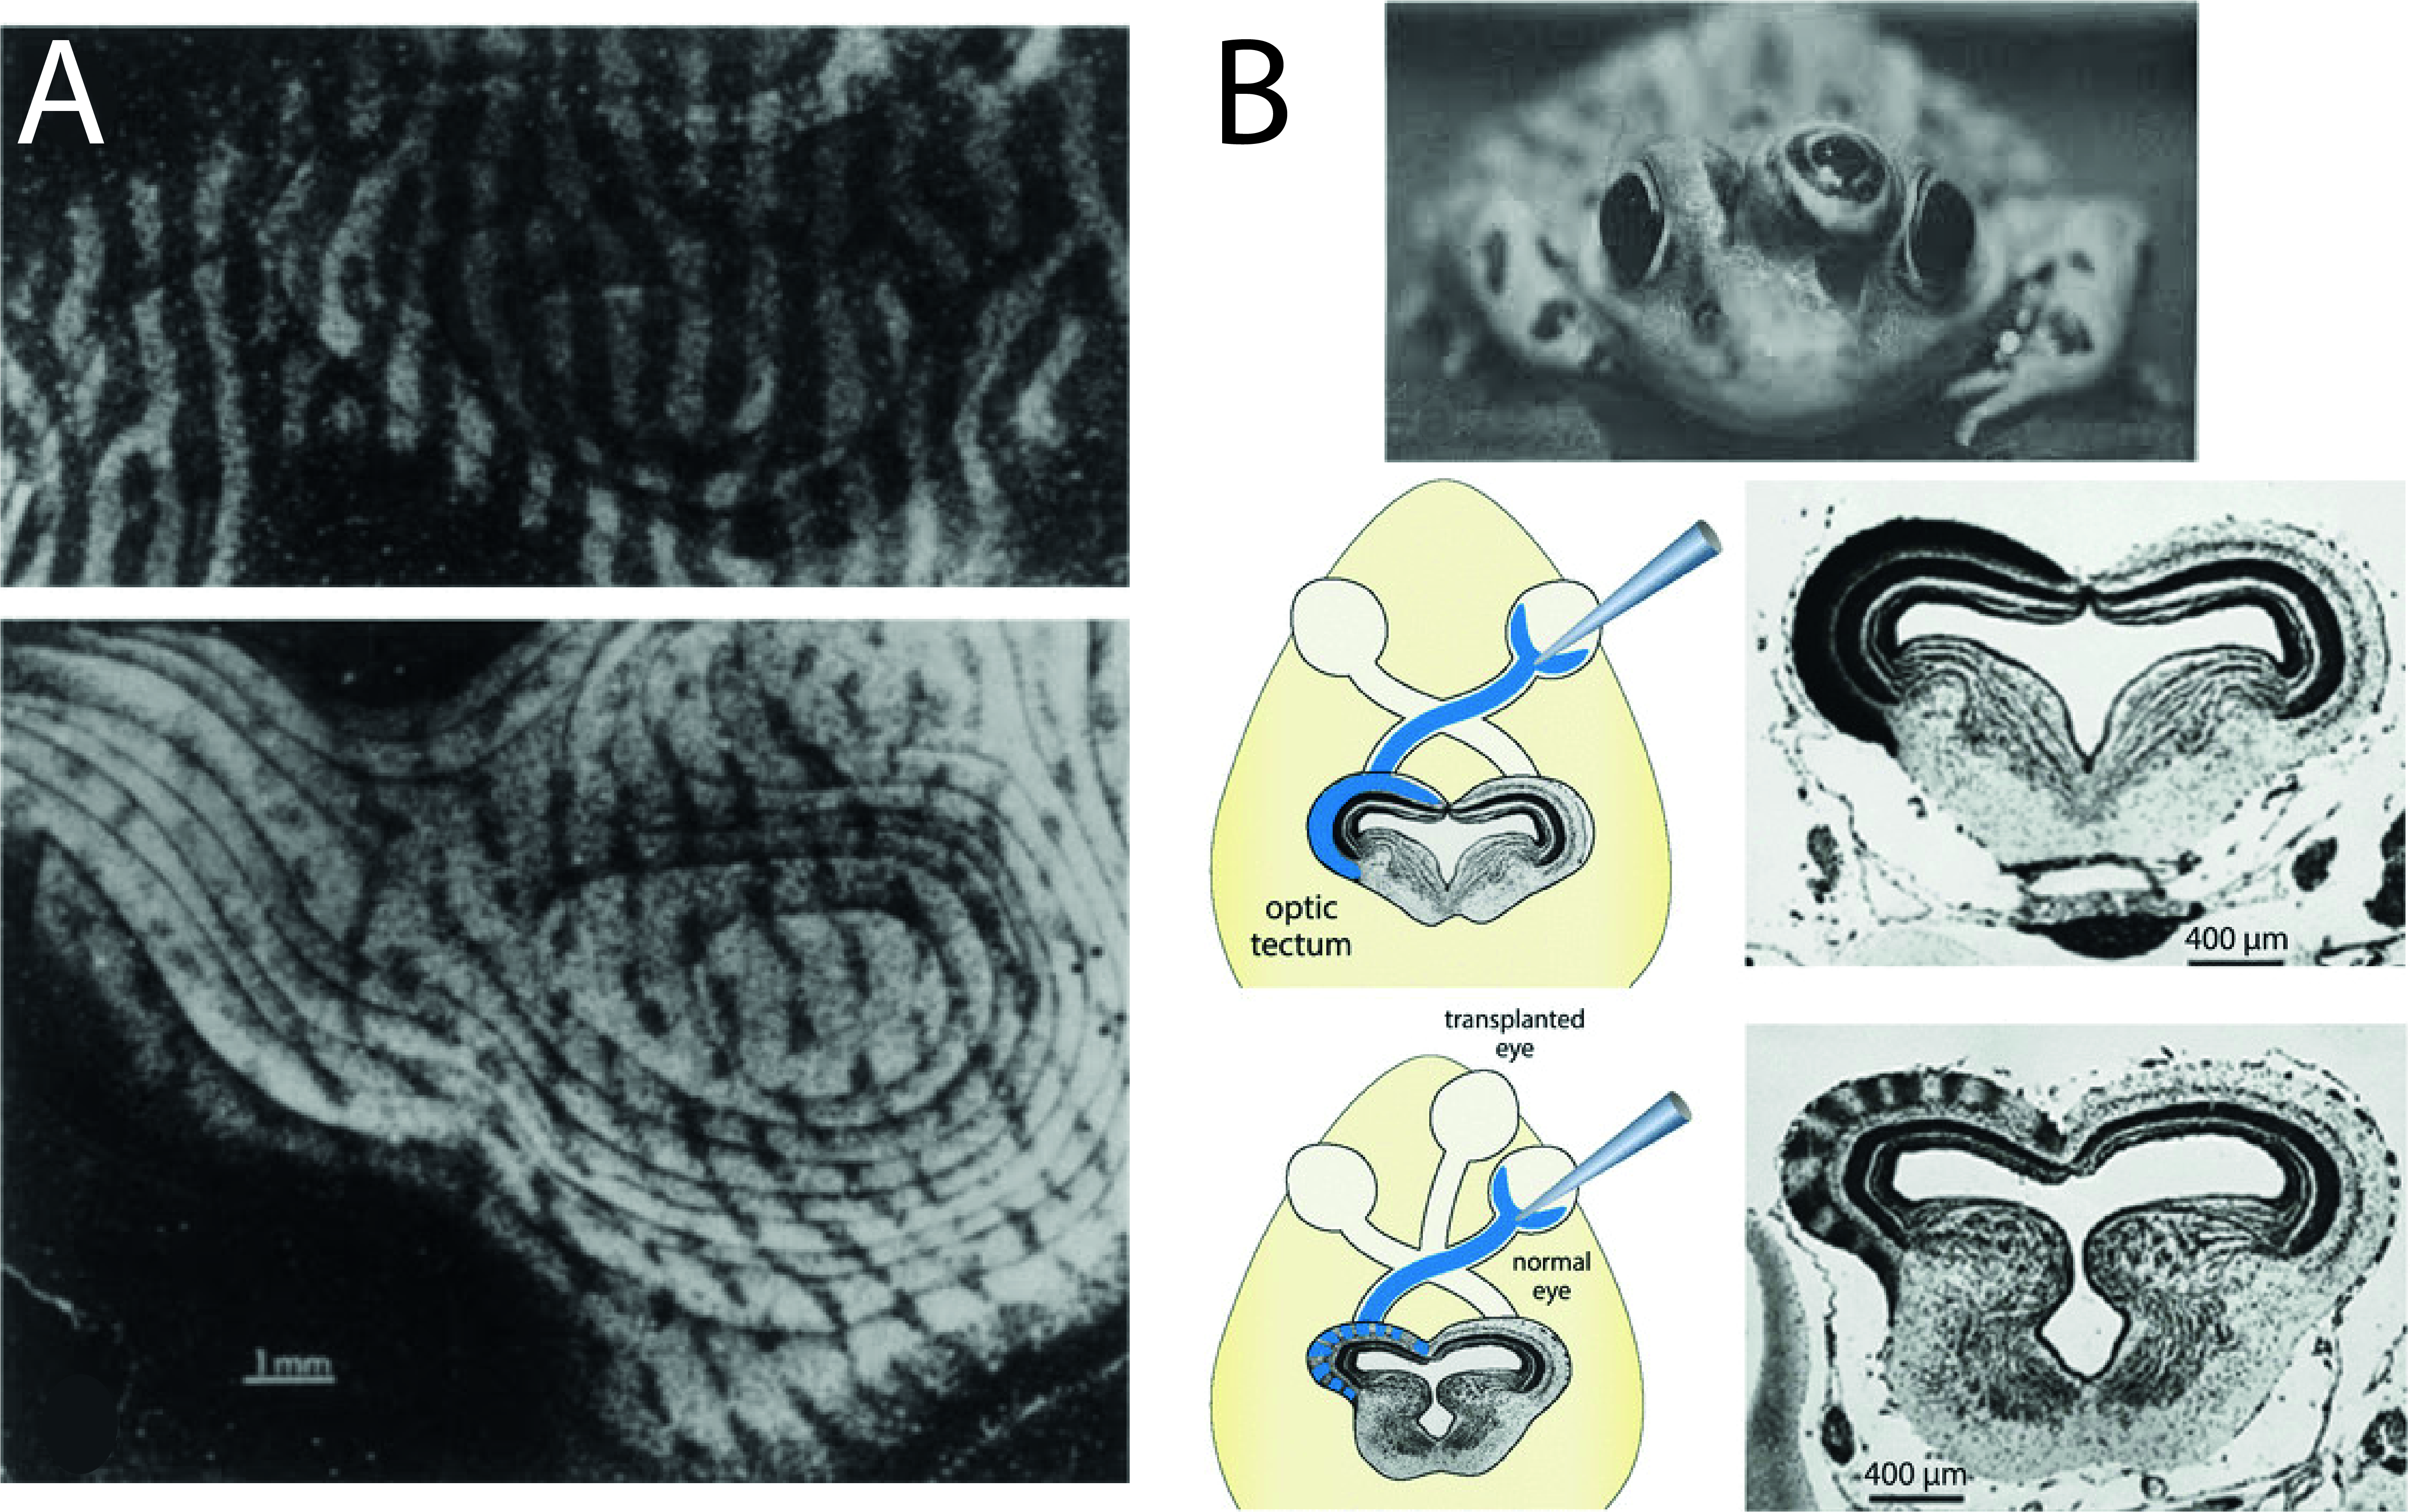
\includegraphics[width =  0.7\paperwidth]{Figures/I_sensory_maps.jpg}}
            \caption[\textbf{\label{fig:I_sensory_maps}\textbf{Sensory maps can be reordered by changing activity patterns.}}]{ \textbf{\label{fig:I_sensory_maps} Sensory maps can be reordered by changing activity patterns.}  \textbf{(A)} Ocular dominance columns in layer 4 V1 of a normal macaque (\textbf{Top}) and in an animal that has undergone MD (\textbf{Bottom}). These were labelled by injecting a radiotracer into the eye with bands corresponding to the labeled eye in white. In the normal animal bands corresponding to either eye are equally sized. In the deprived animal the bands corresponding to the non-deprived eye (white) are expanded, occupying territory that would usually be occupied by the deprived eye (Top: \cite{Hubel1977PlasticityCortex.}, Bottom: LeVay et al., 1980). \textbf{(B)} Top: A three eyed frog, generated by transplanting one supernumerary eye during embryonic stages (\cite{Constantine-Paton1978Eye-specificFrogs}). This results in dual innervation of optic tectum. Middle: In a normal frog injecting a tracer labels into the eye labels only the contralateral tectal hemisphere (black). Bottom: In the three eyed frog injecting the radio tracer into the eye whose RGCs project to the same hemisphere as the supernumerary eye results in segregation of the input from the two eyes.  (\cite{Maya-Vetencourt2013Experience-DependentSystem}).
}
      \end{figure}

\subsubsection{Refinement of retinotopic maps in the optic tectum/SC}

 Early evidence seemed to suggest that activity is dispensable for the initial formation of retinotopic maps in the optic tectum. For example, blocking action potentials in the RGCs by injecting sodium channel blockers, such as \gls{ttx}, into the eye does not affect mapping between retina and tectum, as coarse retinotopic maps still form (\cite{Kobayashi1990DisturbanceGrayanotoxin, Meyer1983TetrodotoxinGoldfish, Olson1991TheProjection}). Additionally, in an imaginative experiment, Bill Harris transplanted an eye from an Axolotl into a \textit{Taricha torosa} newt (\cite{Harris1980TheSalamanders}). This species of newt naturally produces TTX but its neurons are unaffected by the toxin, meaning that only action potentials in the regenerating retinal projections were blocked. Despite the lack of activity in the retina, these projections still formed a crude retinotopic map within the newt tectum. This demonstrates that the initial establishment of retinotopic maps is activity-independent and is driven entirely by molecular cues.

Despite this, the initial topographic map is relatively coarse and has been shown to refine throughout development (\cite{Gaze1974TheXenopus}). More detailed experiments looking at point-to-point mappings within the tectum suggest that refinement is driven activity (\cite{Ruthazer2004InsightsPerspective}). For example, focal injections of neuronal tracers into the eye allow for a small number of developing or regenerating RGCs to be labelled and the area occupied by their terminals to be visualised in the tectum.  For similar sized focal injections into eyes where activity has been blocked by TTX, the area occupied by RGC terminals in the tectum is expanded (\cite{Kobayashi1990DisturbanceGrayanotoxin, Olson1991TheProjection},). Furthermore, this correlates with an expansion of the receptive field sizes on tectal neurons suggesting that the retinotopic map is less precise (\cite{Schmidt1983ActivityGoldfish}).

Some of the strongest early evidence for activity refining retinotectal maps comes from a study in which a third eye was grafted onto developing tadpoles (\cite{Constantine-Paton1978Eye-specificFrogs}). This caused a single tectal hemisphere, which usually exclusively receives projections from the contralateral eye, to be dually innervated by both the existing eye and the transplanted eye. If molecular cues were the only organising mechanism at play, then both eyes, expressing similar guidance cues, should display overlapping retinotopic maps that can be superimposed onto one another. In contrast to this, both eyes appear to segregate into eye specific stripes throughout the tectum, reminiscent of OD columns in the visual cortex (\cite{Law1981AnatomyTecta}) (\textbf{Figure \ref{fig:I_sensory_maps}B}). Similar results can also be produced by other manipulations that reroute retinal projections from the from the eye to the ipsilateral tectal hemisphere (\cite{Straznicky1979AnomalousAblation, Law1980RightAblations}). This indicates that, as the eyes are molecularly indistinguishable from one another, it must be the differences in the patterns of activity between the two eyes that organizes them into the bands. This was further supported through the observation that TTX applications could stop the segregation of inputs and could destabilise existing bands, showing that activity is needed for both their formation and maintenance (\cite{Meyer1982TetrodotoxinGoldfish, Boss1984ActivityGoldfish}). Furthermore, similar effects to those seen with TTX can be produced by blocking N-methyl-D-aspartate glutmate receptors (\acrshort{nmda}) specifically within the tectum showing that it is not only activity but also activation of postsynaptic tectal neurons that is important for organising these inputs (\cite{Reh1985Eye-specificPipiens.}). This implies that activation of postsynaptic neurons can instruct presynaptic input, presumably through a retrograde signal (\cite{Ruthazer2004InsightsPerspective}).

These early experiments raise a fundamental  question, what types of activity are important for driving this refinement? A number of studies have attempted to specifically look at how visual experience contributes to retinotopic map formation. One way to test this is to examine how the retinotopic maps develop in the absence of visual input by rearing the animal in complete darkness. Dark reared goldfish have slightly enlarged tectal multi-unit receptive field sizes, indicative of a more imprecise topographic map (\cite{Schmidt1985StroboscopicGoldfish}). However, in \textit{xenopus} frogs, receptive field sizes of dark reared animals were similar to that of controls (\cite{Keating1986VisualLaevis}). Additionally, dually innervated tecta of zebrafish still produce eye segregated bands when dark reared (\cite{Ramdya2008EmergenceCircuit}). While this may, as a first pass, suggest that visual experience does not contribute to retinotopic map formation, other manipulations of the visual scene have been found to have a much larger impact. For example, stroboscopic rearing, where flashes of light create correlated patterns of activity across the visual field, has been used to look at developing and regenerating retinotopic maps in fish (\cite{Schmidt1993ActivitydrivenSharpening, Schmidt1985StroboscopicGoldfish}). In both cases this led to enlarged receptive fields of tectal neurons and enlarged RGC terminals that failed to refine, suggesting that visual experience plays an instructive role on retinotopic map formation. However, perhaps the most compelling demonstration that visual experience shapes the retinotopic map relied on the observation that as frogs and fish swim forward, optic flow would induce activity in the retina in the temporal to nasal directions (T to N) (H\cite{Hiramoto2014OpticInformation}). Exposure to T to N optic flow in young tadpoles when the retinotopic map is poorly defined, results in the development of precise topography whereas when it is in the opposite direction (N to T) the map is poorly organised. This indicates that it may be specific types of visual experience that are important for instructing the formation of retinotopic maps.

As mentioned above, dark rearing appears to have a limited effect on establishing retinotopy compared to other manipulations of the visual scene. A potential reason for this is that dark rearing does not eliminate spontaneous activity. In mammals, spontaneous retinal waves are propagated through RGC terminals to the SC where they are thought to refine the topographic map (\cite{Pratt2016AnDevelopment}). A large amount of evidence for this hypothesis has been generated using the Chrnb2 \gls{ko} mouse (\cite{Rossi2001RequirementSystem,McLaughlin2003RetinotopicDevelopment,Mrsic-Flogel2005AlteredWaves}). This mutant lacks a subunit of the nicotinic acetylcholine receptor, which is required for the generation of Type II cholinergic waves. Retinal waves in this mutant lack a defined wave front, are more infrequent, and are more spatially distributed appearing as “flashes” across the retina (\cite{Burbridge2014VisualReceptors}). As a consequence retinotopic maps in the SC of these mutants are disrupted alongside deficits in eye specific segregation of RGC axons in the SC (\cite{McLaughlin2003RetinotopicDevelopment, Rossi2001RequirementSystem,Mrsic-Flogel2005AlteredWaves}). The overall activity level within the retina can be restored through either optogenetic or pharmacological manipulations, which rescue the deficit in eye segregation but not retinotopy (\cite{Zhang2012, Burbridge2014VisualReceptors}). In contrast to this, the Rx-$\beta$2 \gls{cko} mouse has lower overall activity in the retina but retains high local correlations between RGCs (\cite{Xu2015SpatialFrequency}). This mutant has eye segregation defects but retinotopic maps in the SC are indistinguishable from those in \gls{wt} mice. Together these studies indicate that it is the local correlational structure of retinal waves, rather than overall activity levels, that are important for organising retinotopy in the SC. Based on this it is possible that spontaneous activity that is seen in the retina of fish may compensate for the lack of visual experience in dark reared animals, allowing for retinotopic maps to still be refined (\cite{Kutsarova2017RulesBrain}). Interestingly, although retinal waves are not usually observed in frogs, dark rearing can induce increased local correlations between neighboring RGCs (\cite{Demas2012VisionRetina}), suggesting that there may in fact be common evolutionary mechanisms for coping with the absence of patterned visual input during development (\cite{Pratt2016AnDevelopment}).

\subsection{Activity regulates neuronal morphology and growth.}
Many observations which have demonstrated that activity shapes sensory maps have relied on bulk labeling of neurons using fluorescent or radioactive tracers. These have allowed for gross anatomical changes in neuroanatomy to be observed (\cite{Berry2016Experience-DependentSystem}). However, underlying these large scale changes are more subtle rearrangements in both axonal and dendritic arbours, altering neuronal structure and their connectivity with their neighbours. In the case of OD, individual thalamocortical neurons can be labeled in order to understand the effect of MD on the structure of axon terminals. This revealed that, after brief MD, the axonal arbours of afferents from the deprived eye begin to shrink (\cite{Antonini1993RapidCortex}). With longer periods of MD, it is found that the afferents of the non-deprived eye expand their territories, accounting for the population scale changes in OD columns (\cite{Antonini1996PlasticityCat.}). This suggests that the level of activity of a neuron may regulate the size of its arbour. 

The level of activity has also been found to be important for regulating RGC arbor size in zebrafish by genetically altering the level of activity in developing RGCs. For example, in the \textit{macho} mutant line of zebrafish, developing RGCs exhibit reduced sodium currents between 4-6 days \gls{dpf}, a period during which the retinotopic map is undergoing refinement (\cite{Gnuegge2001AnalysisMap}). The consequential silencing of RGCs leads to more extensive terminal abours, suggesting that they fail to refine in an activity-dependent manner. Similarly, the \textit{blumekhol} mutant expresses a mutated form of a vesicular glutamate transporter (vglut2a) in RGCs (\cite{Smear2007VesicularZebrafish}). This reduces glutamatergic release from RGCs and results in a similar phenotype to the macho mutant with larger terminal RGC arbours. This further indicates that “cross-talk” between developing RGCs and tectal neurons through synaptic activity is likely to be important for organising these inputs.

More nuanced manipulations have suggested that it is not simply the activity of neurons that shapes their growth, but their activity relative to their neighbours through competitive interactions. This can be shown by genetically silencing the activity of single RGCs, in an otherwise intact tectum. In one study, single RGCs were either hyperpolarized through the overexpression of an inward rectifying potassium channel, Kir 2.1, or were synaptically silenced through the expression of a dominant negative form of vesicle associated membrane protein (\cite{Hua2005RegulationCompetition}). Both manipulations resulted in a reduction in axon motility, leading to reduced total arbour length and branching complexity. Interestingly, this phenotype can be rescued if activity in neighbouring neurons is also suppressed. This suggests that decreased neural activity relative to neighbouring neurons leads to restricted growth. However, a more recent study, which also silenced synaptic activity in single developing RGCs through the expression of exogenous tetanus toxin, found the opposite effect (\cite{Fredj2010SynapticProjection}). Rather than reducing in size, the developing arbours failed to arrest growth resulting in an increase in total arbour length, although this effect could also be rescued through the suppression of neighbouring neurons. One potential reason for this is that these studies utilise different genetic promoters, potentially labelling different RGC subtypes. This hypothesis suggests that activity plays different roles in modulating arbour extensions in different cell types. Alternatively, the degree of silencing by each of these manipulations may be differ ultimately leading to different effects on arbour length and branching complexity. Regardless, both studies restore the arbour size to that of controls by inhibiting neighbouring neurons (\cite{Kita2015TopographicZebrafish}). This reaffirms that it is the level of activity relative to its neighbours that is important for shaping arbour growth, through a competitive interaction between neurons. 

\subsubsection{Activity dependent synaptotropic growth}
Time-lapse imaging in fish and frogs allows for the structure of singly labelled RGC axons and tectal dendrites to be visualised as they are growing, allowing for detailed studies into how activity affects arbour growth (\cite{ORourke1990DynamicStudy, Kaethner1992DynamicsAxons}). This has demonstrated that developing arbours go through a rapid phase of growth within the first few days and followed by a plateau (\cite{Wu1999DendriticMaturation, Cline2001DendriticSynaptogenesis, Meyer2006EvidenceMechanisms, Niell2004InArbor}). Within the initial growth period, arbours are highly dynamic, extending and retracting motile small filopodia with only a small fraction of these arbours being retained and stabilized. Even once the growth plateaus, branches are still extended and retracted at a slower rate and receptive fields of tectal neurons continue to refine suggesting that synaptic inputs are still being remodelled (\cite{Zhang2011FunctionalZebrafish}). A number of studies have highlighted that axon and dendrite growth is regulated by the formation of synapses, through a process of synaptotropic growth (\cite{Niell2004InArbor, Ruthazer2006StabilizationMaturation, Meyer2006EvidenceMechanisms}). Under this process, developing arbors send out large numbers of filopodia,  sampling the surrounding area and making nascent synapses. Only those that make the correct contacts are maintained, forming more mature synapses, whereas incorrect contacts are eliminated. These newly matured synapses then serve as branch points for newly extending filopodia.  Synaptotropic  growth therefore allows a developing arbour to preferentially explore a region where there is more likely to be correct contacts (\cite{Cline2001DendriticSynaptogenesis}). 

The stabilization of “correct contacts” is thought to be driven by correlated visually evoked activity between neurons (\cite{Ruthazer2006StabilizationMaturation}) through the activation of the NMDAR (\cite{Ruthazer2003ControlVivo}), the only glutamatergic receptor present at early/nascent synapses. Consistent with this, imaging a single developing axon in tadpoles that have dually innervated tecta suggests this dynamic process of growth is modulated by correlated activity between neurons (\cite{Ruthazer2003ControlVivo}). Here, the developing RGCs extend their filopodia with equal probability in all directions but branches are eliminated at a higher rate in territories that are occupied by the opposite eye. This suggests that branches are preferentially stabilized in regions of higher correlation that are occupied by RGCs from the same eye, which underlies the formation of eye specific bands. This process relies on postsynaptic glutamate activity since  blocking NMDARs abolishes this preferential stabilisation. In addition, Munz et al., (2014) took advantage of stray ipsilateral retinotectal projections to look at the effects of synchronous vs asynchronous visual stimulation to each eye on arbour growth. Here, synchronous activity between the two eyes promoted synapse formation in the stray axon, leading to similarly sized arbours as those in the contralateral projection. Asynchronous stimulation, on the other hand, resulted in a rapid increase in both branch additions and eliminations. This occurred alongside a decreased synaptic drive onto tectal neurons, suggesting that synapses are not mature. This shows correlated activity is required for the maturation of synaptic contacts and for the stabilization of developing branches, an effect that can be mimicked by NMDAR blockage (\cite{Munz2014RapidStimulation}). Together these experiments suggest that growth is directed by synapse formation in regions of correlated visual activity, in a process that is NMDAR dependent.

As RGC arbours are elaborating so must the dendritic arbours of their postsynaptic partners. It is therefore not surprising that tectal dendrites are equally as dynamic during development and also display highly heterogeneous branching patterns. Throughout this growth, tectal neurons receive synaptic input from the retina, suggesting that synaptic activity may be able to modulate this growth process. Consistent with this, blocking glutamatergic activity using NMDAR antagonists stops dendritic growth in the early stages of tectal development (\cite{Rajan1998GlutamateVivo}). To understand if visual experience has a direct role in modulating the growth of dendritic arbours, tectal neurons were timelapse imaged in vivo following 4 hour periods of either total darkness or the exposure to a moving stimulus (\cite{Sin2002DendriteGTPases}).   Imaging the same neurons within both conditions allows for comparison of growth rates, which enables subtle changes in growth to be examined that would otherwise be missed when averaging across populations. This revealed that exposure to visual stimuli promotes dendritic arbour growth, whereas in periods of darkness arbour growth is slowed. Furthermore, this change in dendritic motility could be blocked via the application of NMDAR antagonists, showing that glutamatergic synaptic inputs regulate these  experience-dependent changes.  Therefore these experiments show that activity, and through visual experience in particular, is integral for shaping neurons morphology and growth. 


\subsection{Receptive field properties are shaped by activity}
\subsubsection{Orientation selectivity}
 By shaping the physical structure of neurons, activity serves to alter connectivity within the visual system. This changes the input onto neurons, which is important for shaping their receptive field properties. Throughout the visual pathway neurons have been found to be specifically tuned to the orientation of edges and lines (\cite{Hubel1968ReceptiveCortex, Passaglia2002, Niell2008HighlyCortex,Nikolaou2012ParametricTectum,Fisher2015OrientationDrosophila}). Although these orientation selective neurons are wide-spread among vertebrate species, their development has been most studied in the visual cortex of mammals. In carnivores specifically, orientation tuning is mapped across the cortex where neurons with similar orientation preferences are clustered together (\cite{Maldonado1997OrientationCortex}). Optical imaging in ferrets has shown that orientation bands are present two weeks prior to eye opening and adult-like levels of tuning are achieved one week after the eyes open (\cite{Chapman1999DevelopmentCortex}). Blocking retinal activity through TTX injections blocks the development of orientation selectivity in the cortex (\cite{Chapman1993DevelopmentDeprivation}). However, disentangling the role of visual experience and spontaneous activity is complicated by the fact that visual activity can be evoked through the eyelid, although the pattern of stimulation is distorted (\cite{Krug2001ResponsesLids, Spear1978StriateEyelids}). In light of this, animals have been dark reared prior to eye opening and orientation selectivity populations are still present, suggesting that spontaneous retinal activity is sufficient for initially establishing orientation selectivity (\cite{White2001TheCortex}). Consistent with this, artificially disrupting the structure of spontaneous activity by pharmacologically inhibiting ON-RGCs (\cite{Chapman2000CorticalActivity}) or stimulating the optic nerve (\cite{Weliky1997DisruptionActivity}) can drastically alter the emergence of orientation selectivity. After eye opening, dark rearing can inhibit the maturation of orientation selectivity in ferrets (\cite{White2001TheCortex}). However, double eye-lid suturing, which distorts the visual experience, results in a far more severe effect with orientation selectivity being nearly absent in this group (\cite{Chapman1993DevelopmentDeprivation, White2001TheCortex})(\textbf{Figure \ref{fig:I_OS_DS_f}A}). Together these experiments suggest that it is not the mere presence of visual experience that is important for the maturation of orientation selectivity, but the pattern that is caused by normal visual stimulation. 
 
In addition to the effects of sensory deprivation, a number of studies have investigated the plasticity of orientation selectivity in the cortex by stripe rearing, a procedure where animals are raised in visual environments containing contours of a single orientation. Typically this has been done by either rearing animals in striped cylinders or raising them wearing goggles that restrict the orientations that the animal is exposed too (\cite{Blakemore1970, Stryker1975ModificationReexamination, Freeman1973AlterationAsymmetries}). Electrophysiological studies in cats have led to mixed reports, with high variability in effects between studies and also between animals within the same study , potentially reflecting the sampling bias associated with single cell recordings (\cite{Blakemore1970, Stryker1975ModificationReexamination, Blakemore1977GeneticCortex.}). In contrast, optical imaging in ferrets shows low variability and demonstrates that, while all orientations are represented, there is a large over-representation for the experienced orientation (\cite{Sengpiel1999InfluenceCortex}). Similar effects of stripe rearing have also more recently been seen in the visual cortex of mice with single cell resolution optical imaging (\cite{Kreile2011AlteredCortex}). This shows that the responses of neurons can be shifted towards the experienced orientation, suggesting that visual experience can play an instructive role in shaping orientation selectivity. 

\subsubsection{Direction Selectivity}
Just as neurons exhibit orientation selectivity, a substantial proportion of cells within the visual system respond significantly more to stimuli moving in a particular direction than to motion in the opposite direction, known as direction selectivity. Unlike orientation selectivity, direction selective neurons are absent from the visual cortex of ferrets at the time of eye opening and emerge two weeks after eye opening. This development is completely driven by patterned visual experience, with dark reared ferrets lacking directional tuning in V1 (\cite{Li2006TheExperience})(\textbf{Figure \ref{fig:I_OS_DS_f}B}). Furthermore, briefly exposing these animals to stimuli moving in a single direction can induce tuning in that direction whilst leaving tuning for all other directions absent. Similar effects of experience on direction selectivity have been found in the optic tectum of \textit{xenopus} tadpoles. While direction selectivity is absent during the early developmental stages, exposing tadpoles to a bar that repeatedly travelled in a single direction can train neurons to respond selectivity to stimuli moving in that direction (\cite{Engert2002MovingNeurons}). This training can be abolished by the application of NMDA antagonists, indicating that it is mediated by synaptic glutamate activity. Together, these results show that visual motion in the environment can play an instructive, rather than permissive, role in the formation of direction selectivity.

Interestingly, this effect of visual experience may be species or brain region specific. This is because dark rearing zebrafish has no effect on the emergence of direction selectivity within RGCs or tectal neurons (\cite{Niell2005FunctionalTectum}; \cite{Ramdya2008EmergenceCircuit}; \cite{Lowe2013ADevelopment}). Similarly, direction selectivity in the superior colliculus of mammals can still emerge when animals are dark reared, although this tuning can be disrupted through strobe rearing (\cite{Chalupa1978DirectionalDark-rearing,Flandrin1975SuperiorKitten}). However, it is not known whether the sustained experience of a particular direction can alter these tuning profiles. 

Together the studies described so far show that many aspects of visual system development are genetically encoded, either through molecular cues specifying projection targets, or by spontaneous activity shaping neural circuits. However, extrinsic activity, driven by visual experience, has been shown to have profound effects on multiple aspects of visual system development including sensory maps, neuron morphology and the receptive field properties of neurons. This indicates that visual experience serves help mature neural circuits, or change their organisation all together. 



\begin{figure}[!ht]
        \center{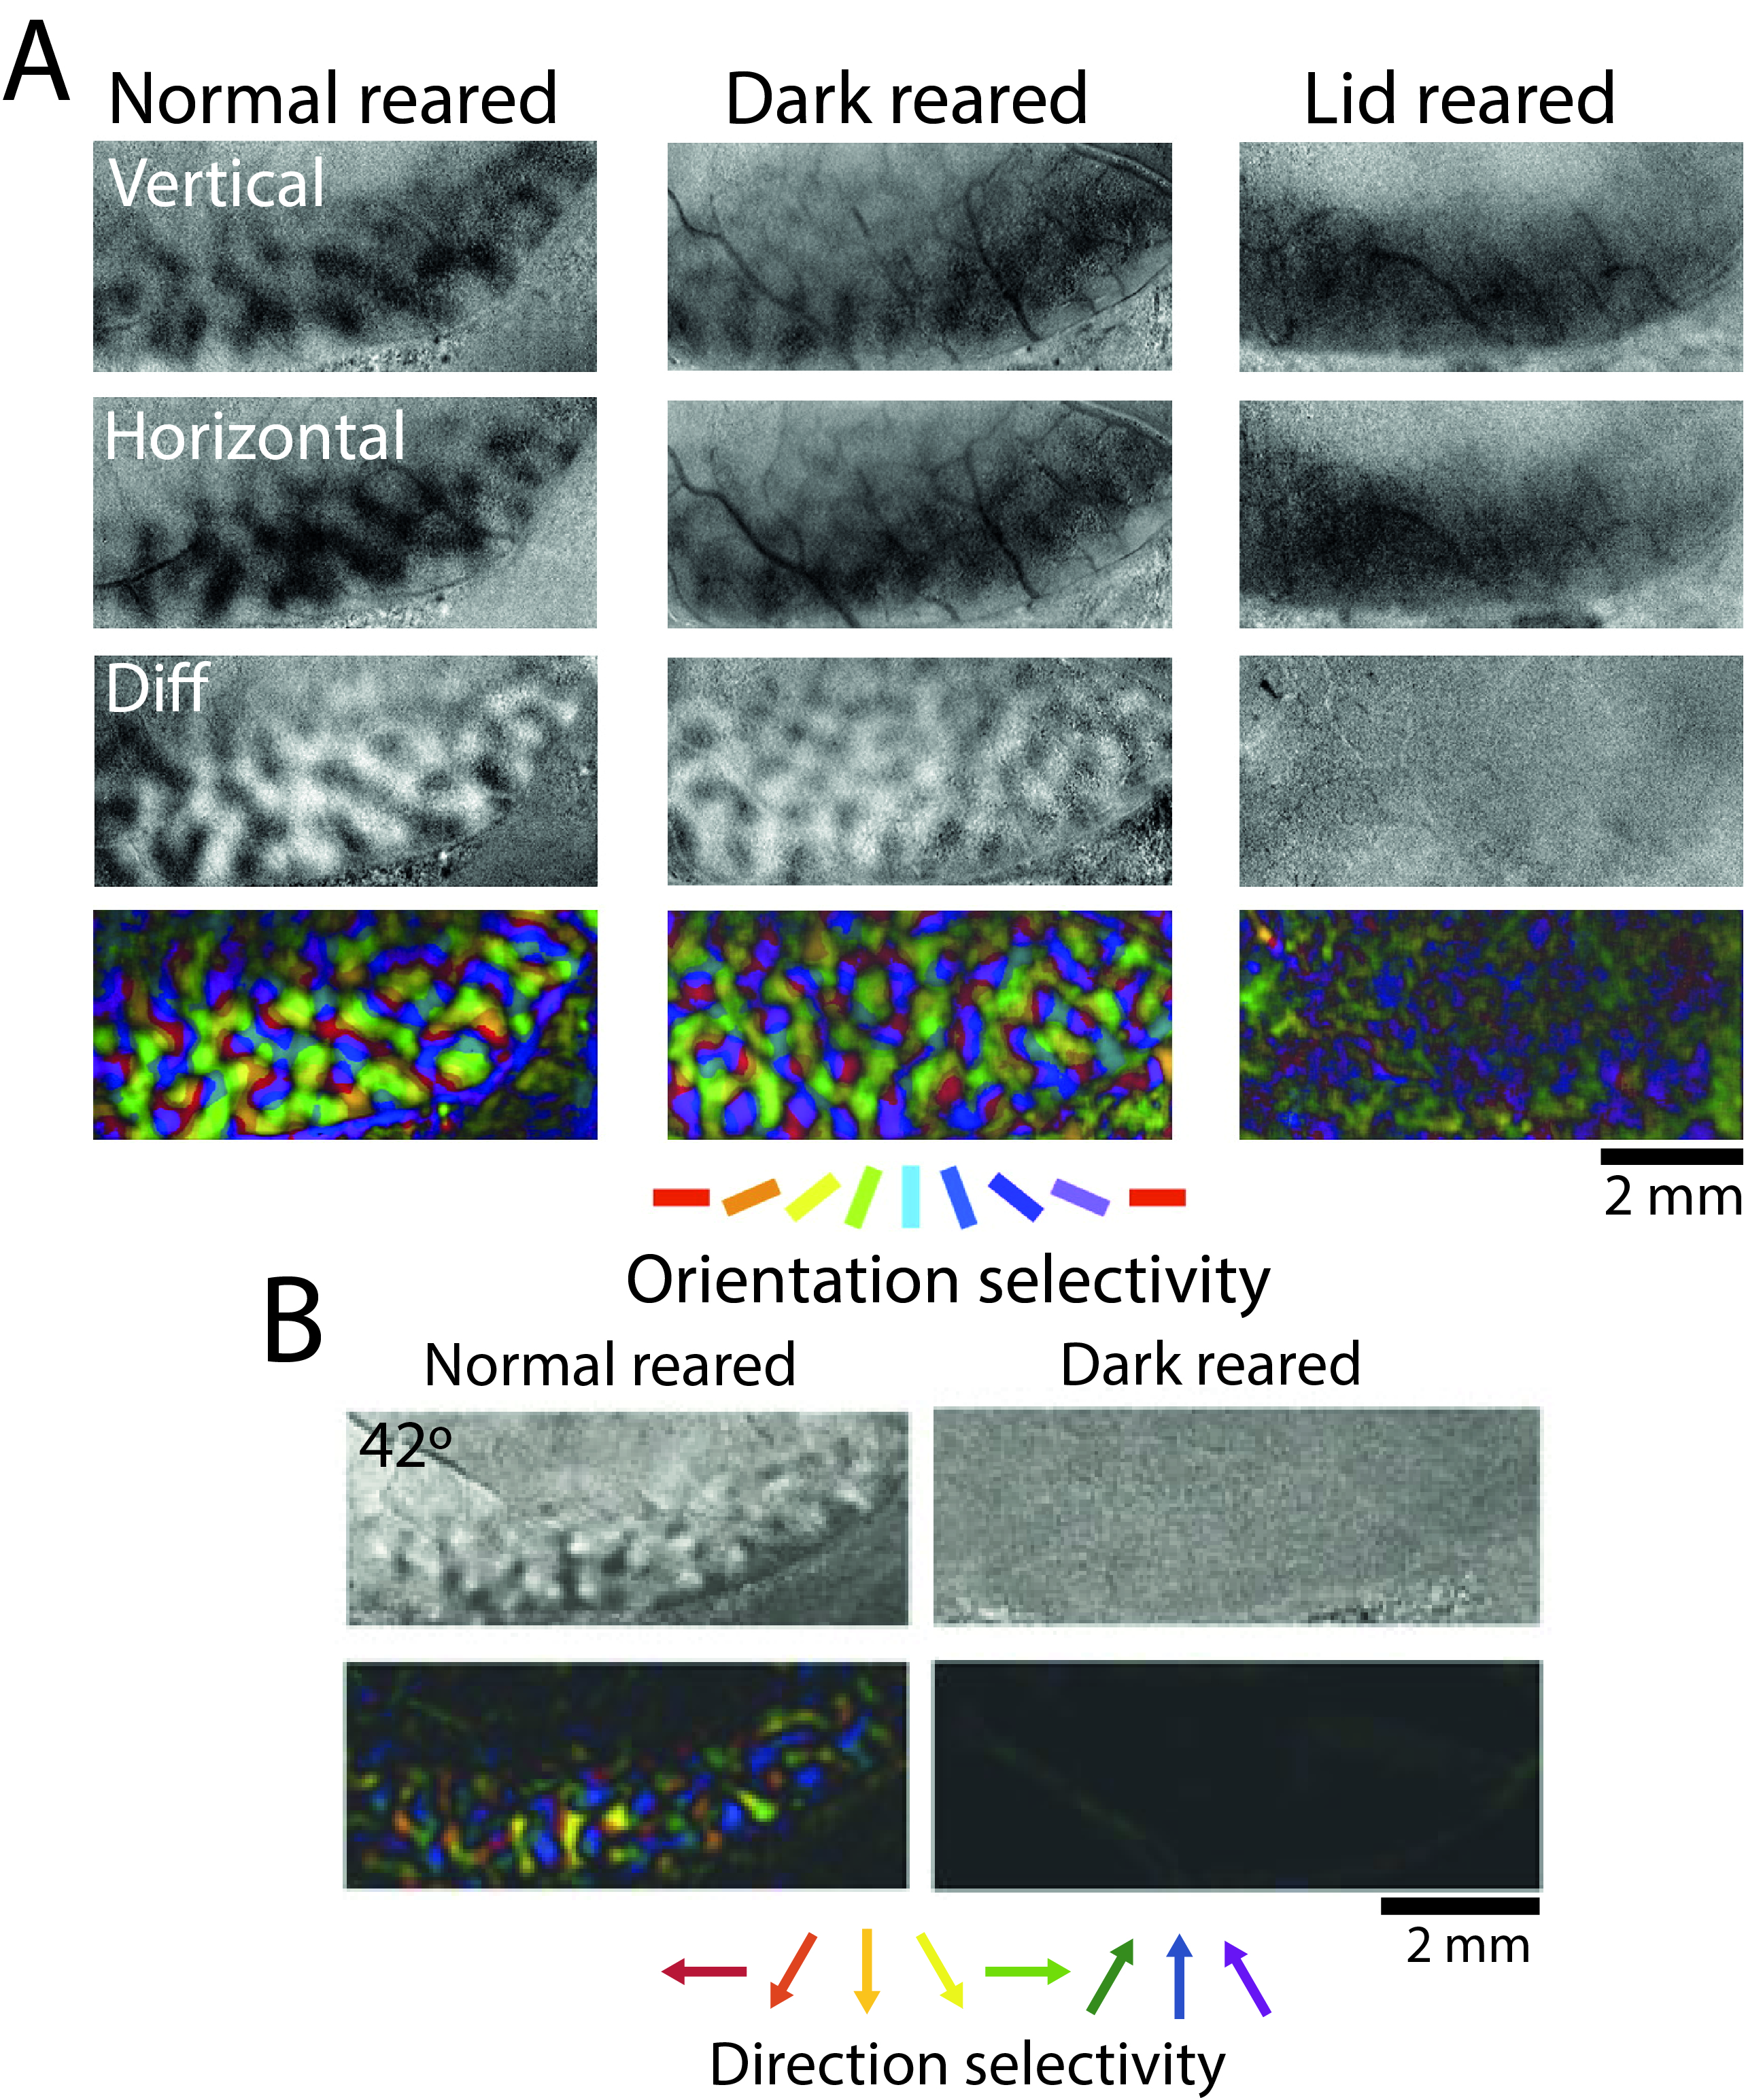
\includegraphics[width =  0.6\paperwidth]{Figures/I_OS_DS_ferrret_2.jpg}}
            \caption[\textbf{\label{fig:I_OS_DS_f}\textbf{The effect of visual experience on the development of receptive field properties in the cortex. }}]{\textbf{\label{fig:I_OS_DS_f} The effect of visual experience on the development of receptive field properties in the cortex.} \textbf{(A)} Optical imaging of changes in the haemodynamic response in V1 to stimuli of different orientations in ferrets that have been normally reared (\textbf{left column}), dark reared (\textbf{middle column}) or lid sutured (\textbf{right column}). \textbf{Top row:} shows mean response to vertical stimuli. \textbf{Second row:}  the mean response to horizontal stimuli. textbf{third row:}  the difference between them. \textbf{Bottom row:} shows the maximum response to each orientation as color coded by legend. This shows that while orientation selectively is reduced in the dark reared group, it is almost absent in the lid sutured group. Thus, while visual experience is important for the maturation of orientation selectivity, abnormal patterns of visual stimulation can disrupt it. Images from (\cite{White2001TheCortex}). \textbf{(B)} Optic imaging of the haemodynamic response in V1 to stimuli moving in different directions in ferrets that have been normal reared (\textbf{left column}) or dark reared (\textbf{right column}). \textbf{Top row:} shows the mean response to stimuli moving at 42 degrees (0 degrees = horizontal moving rightward). \textbf{bottom row:} A map colored by max response to each direction. This demonstrates that direction selectively does not form in dark reared animals (\cite{Li2006TheExperience}). 

        }
      \end{figure}



\subsection{Hebbian plasticity and the NMDAR}
A core conceptual framework underlying many of the activity-dependent changes discussed above is that of Hebbian plasticity. Hebbian plasticity is the notion that correlated firing between pre- and postsynaptic neurons causes an increase in the synaptic efficacy between them  (long term potentiation - LTP) whereas decorrelated activity between neurons leads to decreased synaptic efficacy (long term depression - LTD) (\cite{Hebb1949, Stent1973ALearning.}) (\textbf{Figure \ref{fig:I_hebbian_plasiticty_fig}A}). Confirmation of Hebb’s rule in hippocampal cultures indicated that high frequency tetanic stimuli could induce LTP whereas low frequency stimulation resulted in LTD (\cite{Bliss1973LonglastingPath, Kemp2004HippocampalAccquisition,Dudek1992HomosynapticBlockade}). In addition to this, experiments in the optic tectum of frogs suggested that synaptic plasticity could be bidirectionally regulated by the relative timing of pre- and postsynaptic spikes (\cite{Zhang1998ASynapses}). In these experiments, tectal cells were patched alongside RGCs allowing for controlled stimulation of these neurons relative to each other. By shifting the relative timings between pre- and postsynaptic neurons, it was shown  that LTP could be induced if the RGC fired prior to the tectal neuron, whereas LTD was induced if this order is reversed. The extent of this synaptic modulation was found to be asymmetrically proportional to the time interval relative to the postsynaptic spike, exponentially decaying over a 10 msec time window,  a phenomenon known as \gls{stdp} (\cite{Mu2006SpikeSystem}) (\textbf{Figure \ref{fig:I_hebbian_plasiticty_fig}B}).  This gives a mechanism by which temporally organised spiking patterns can shape synaptic connectivity. Importantly, different visual scenes contain different statistics, producing unique spiking patterns. Therefore, Hebbian mechanisms potentially underlie the instructional influence that the visual environment exerts over the developing visual system. Consistent with this, LTP can be induced through visual stimulation (\cite{Zhang2000VisualSynapses}) and Hebbian plasticity has been implicated in numerous aspects of experience-dependent development in the visual system, including the formation of retinotopic maps (\cite{Ruthazer2003ControlVivo}), neuron growth (\cite{Munz2014RapidStimulation, Sin2002DendriteGTPases}), and direction selectivity (\cite{Engert2002MovingNeurons, Mu2006SpikeSystem}).

A critical component of the Hebbian framework is the NMDAR, an ion channel situated on the postsynaptic membrane that is usually occluded by a Mg2+ ion at rest. The channel requires both binding of glutamate released from the presynaptic neurons and depolarisation of the postsynaptic neuron to occur in order to relieve this block, allowing current to influx (\cite{Nowak1984MagnesiumNeurones}) (\textbf{Figure \ref{fig:I_hebbian_plasiticty_fig}C}). This property of the channel allows it to act as a molecular detector of correlated activity between pre- and postsynaptic activity (\cite{Yashiro2008RegulationMetaplasticity}). Notably, NMDAR antagonists have been shown to abolish LTP formation through STDP rules in vivo (\cite{Zhang1998ASynapses}). When the channel is activated, Ca2+ flows into the cell and triggers intracellular cascades that can lead to synaptic modification. It is thought that the amount of calcium influx is important for the direction of plasticity, with large calcium influx resulting in LTP and small influx causing LTD (\cite{Yashiro2008RegulationMetaplasticity}). In the developing brain, LTP leads to synapse maturation and stabilisation by activating \gls{camkii} which triggers an intracellular cascade.  This cascade causes glutamatergic channels \gls{ampa} receptors to the synaptic membrane,  potentiating subsequent synaptic currents (\cite{Wu1996MaturationSynapse,Wu1998StabilizationCaMKII,Rajan1998GlutamateVivo}). LTD, on the other hand, leads to a reduction in AMPA currents (\cite{Munz2014RapidStimulation}). This mechanism may therefore underlie the selective stabilization of axonal and dendritic branches in regions of correlated activity via synaptotropic growth. Over time, this stabilisation within coactive environments and elimination from non-correlated areas could refine retinotopic maps or eye-specific territories (\cite{Ruthazer2003ControlVivo, Munz2014RapidStimulation}). Consistent with this, NMDAR activity induced by visual experience can lead to modifications in cytoskeletal dynamics via GTPase activity, thereby altering neuron morphology (\cite{Sin2002DendriteGTPases}). Visual experience has also been found to increase glutamatergic synaptic strength by increasing its AMPA receptor contribution, or by shifting AMPA/NMDAR ratio at synapses (\cite{Engert2002MovingNeurons}). Furthermore, inhibiting AMPA trafficking has been shown to block experience-dependent dendritic arbour growth in tectal neurons (\cite{Haas2006AMPAVivo}). Therefore, Hebbian plasticity, facilitated by the NMDAR, gives a mechanism by which neural activity can shape neural connectivity in the developing brain.

\subsubsection{Synaptic plasticity is regulated by NMDAR subunit composition}

The amount of calcium that flows through the NMDAR, and therefore the direction of synaptic plasticity, is  dependent on the subunit composition of the NMDAR (\cite{Yashiro2008RegulationMetaplasticity}). NMDAR are heteromeric tetramers containing two obligatory NR1 subunits and two regulatory subunits that can be N2RA-D or NR3A-B (\cite{Cull-Candy2004RoleSynapses., Al-Hallaq2007NMDAHippocampus}). The majority of the NMDAR’s functional diversity comes from the NR2 subunits. Of these, NR2A and NR2B are most studied due to their elevated expression within the brain, and their differential current kinetics (\cite{Yashiro2008RegulationMetaplasticity}). NR2A-containing synapses have higher opening probability and faster deactivation than NR2B-containing synapses (\cite{Chen1999Subtype-dependenceProbability,Monyer1994DevelopmentalReceptors, Erreger2005Subunit-specificProfiles}). Despite this lower opening probability, the NR2B, due to its slow deactivation, carries around two-fold Ca2+ current through a longer current decay (\textbf{Figure \ref{fig:I_hebbian_plasiticty_fig}D}). Therefore, activation of these different receptors alters the amount of Ca2+ influx through the receptor pore, potentially modulating the direction of plasticity.  The precise relationship between NR2 subunits and the induction LTP/LTD remains controversial (\cite{Liu2004RolePlasticity, Massey2004DifferentialDepression}). However, it has been suggested that, while either subunit can facilitate both forms of plasticity, the NR2A/NR2B ratio at a synapse controls the threshold for synaptic plasticity, acting as a form of metaplasticity over synaptic plasticity (\cite{Philpot2007ObligatoryCortex,Yashiro2008RegulationMetaplasticity}). Under this hypothesis, NR2A dominated synapses are more likely to undergo LTD than those that are dominated by NR2B.

In the mammalian brain, the NR2A/NR2B ratio varies between brain regions and developmental stages (\cite{Cull-Candy2001NMDADisease}).  In the cortex, there is a developmental switch in which NR2B is expressed as the dominant subunit in the first postnatal week and NR2A expression increases shortly after (\cite{Monyer1994DevelopmentalReceptors};  \cite{Sans2000ASynapses, Sheng1994ChangingCortex}). Consistent with this expression pattern and the kinetics of the channels, NMDAR currents at cortical synapses have faster kinetics and a reduced sensitivity to NR2B selective channel blockers at later stages of development (\cite{Carmignoto1992Activity-dependentCortex, Flint1997, Tovar1999TheVitro}). The precise timing of this switch is thought to be regulated by neuronal activity and sensory experience. In dark reared animals, the expression of NR2A in the visual cortex is delayed but can be rapidly induced by just 1 hour exposure to visual experience (\cite{Quinlan1999BidirectionalDevelopment, Carmignoto1992Activity-dependentCortex,Quinlan1999RapidVivo,Philpot2001VisualCortex}).
This switch in NR2B/NR2A composition during development is thought to be crucial for mediating activity-dependent changes in the developing brain. Consistent with this, knocking out the NR2A subunit in mice can keep synapses in an immature state, retaining the longer NMDA currents of NR2B-containing synapses (\cite{Fagiolini2003SeparableSignaling}). In this mutant, the number of orientation selective neurons in the visual cortex is severely reduced. This may suggest that under normal conditions, the developmental switch shifts synapses towards LTD, refining the receptive field properties of neurons. Furthermore, genetic mutations in the \textit{Grin2a} gene, which encodes the NR2A subunit, have been associated with epilepsy in humans (\cite{Gao2017AAphasia}), Suggesting that correct NR2A function is important for shaping developing neural circuits in the brain.

The role of NMDA subunit composition in regulating the development of neural circuitry in non-mammalian vertebrates is virtually unknown, but the NR2A and NR2B subunits are extremely well conserved across species (\cite{Ewald2009CloningTadpoles}). The expression of NR2A is also found to lag behind that of the NR2B in zebrafish (\cite{White2017AZebrafish}). Knocking down the expression of the NR2A subunit in \textit{xenopus} tectal neurons reduces branch clusters, whereas knock down of the NR2B subunit has no effect (\cite{Ewald2008RolesVivo}). Therefore, it is possible that these subunits are important for shaping activity-dependent development of the visual system in different ways within these species. One of the aims of this thesis is to understand how this subunit composition facilitates experience-dependent in developing neural circuits.


\begin{figure}[!ht]
        \center{\includegraphics[width =  0.7\paperwidth]{Figures/I_hebbian_plasiticty_fig.jpg}}
            \caption[\textbf{\label{fig:I_hebbian_plasiticty_fig}\textbf{Visual experience can cause synaptic changes through Hebbian plasticity.}}]{ \textbf{\label{fig:I_hebbian_plasiticty_fig} Visual experience can cause synaptic changes through Hebbian plasticity.} \textbf{(A)} Hebb’s rule: When neurons are correlated in their firing pattern (such as neuron A and B) the synapses between them get stronger through a process of LTP. Neurons that are decorrelated in their firing patterns (neuron A and C) result in weakening of synapses through LTD. \textbf{(B)} A plot showing the change in synaptic strength when the postsynaptic neuron fires at different times relative to the presynaptic neuron ($\delta$t). Here a $\delta$t of 0 indicates that both neurons fire at the same time. When postsynaptic spikes precede the presynaptic spike ($\delta$t < 0), synapses undergo LTD whereas if they follow the presynaptic neurons ($\delta$t > 0), synapse undergo LTP. The extent of the synaptic change exponentially decays as $\delta$t moves away from 0. From (\cite{Bengio2015STDPActivity}). \textbf{(C)} The NMDAR acts as a coincidence detector between pre- and postsynaptic activity, facilitating hebbian plasticity. The pore of the channel is only open when the following two conditions are met: glutamate is bound to the receptor, and the postsynaptic cell is depolarized, removing the Mg2+ blocking the channel, this allows for Ca2+ influx. \textbf{(D)} NMDA channel kinetics depend on the receptors subunit composition. NR1/NR2A NMDAs have a fast opening probability and fast decay kinetics. NR21/NR2B NMDAs have a much slower decay and a lower opening probability. Note that the peak current of NR1/NR2A channels is much higher than NR1/NR2B channels. However, the NR2B containing channel carries around 2-fold the charge overall because of the much longer decay kinetics. Image from  (\cite{Chen1999Subtype-dependenceProbability}).

        }
      \end{figure}

\section{How does natural visual experience influence the formation of visual behaviour and population activity?}

Many of the traditional approaches to studying the effects of visual experience on the developing visual system have relied upon artificial manipulations of the visual input, such as dark rearing, strobe rearing, and stripe rearing. These manipulations have been instrumental in demonstrating that visual experience can instruct the development of the various properties of the visual system, including visual map formation, neuron morphology, and tuning properties of neurons. Furthermore, they suggest that the developing visual system, through modifications in synaptic weights, is able to encode the statistics of the visual environment.  However, the overarching role of the visual system is to drive visual behaviours. Despite this, very few studies examining experience-dependent plasticity in the brain have also looked at behaviour. This maybe due to the fact that in studies were animals have been dark reared, due to the severity of the manipulation, visuomotor behaviour was completely abolished (\cite{Kalil1978DarkNucleus, Mower1982BehavioralCat, Avitan2017}). While this shows that visual experience is required for visual behaviours to develop, it is possible that different types of experience shape behaviours in different ways, potentially even enhancing its performance. In line with this, a small number of studies have shown that visual conditioning can have powerful effects in modifying behaviour on relatively short time scales. For example, following a brief exposure to a moving grating \textit{xenopus} tadpoles have been shown to exhibit more varied levels off acceleration when swimming over counterphased gratings, suggesting that they have improved visual discrimination (\cite{Schwartz2011Activity-DependentDevelopment}). Interestingly, these behavioural changes are reflected by an increased sensitivity of direction selective neurons for the trained direction and this development requires the synthesis of the neurotropic factor BDNF. Interestingly, this same conditioning stimulus can also modify other behaviours with conditioned tadploes being far more likely to swim away from an approaching object (\cite{Shen2014AcuteXenopus}). These studies demonstrate that even a short exposure to certain visual stimuli is capable of shaping behaviour. Based on this it likely that sustained exposure to different visual stimuli through development as the visual system is being assembled could have far more dramatic effects on the ontogeny of behaviour. 

Despite this, no study to date has examined the effect of altered visual scenes during development alongside behaviour. Therefore an aim of this thesis is to do just this, by manipulating the visual scene through \gls{ee} and observe how behaviour is affected. In particular it aims to manipulate the visual scene by mimicking the statistics of visual scenes that would be observed by animals in their natural habitats. If this manipulation has an effect on behaviour, it will be imperative to understand what aspects of brain development may be underlying these effects. To do this, it is important to first consider what aspects of brain function underlie the generation of behaviour in order to look at the most relevant scale. Often due to restrictions in methodology, the effect of visual experience on the development of the visual system has typically been measured by looking at single neurons or sensory maps. However, behaviour is likely to be an emergent property of multiple neurons firing in a distributed populations (\cite{Yuste2005, Saxena2019TowardsDoctrine, Eichenbaum2017}). Therefore, if we want to understand how changes in behaviour are relate to changes in the brain it is necessary to look at developing activity in neural populations. This section introduces the idea of manipulating the visual scene through \gls{ee} and previous attempts to study the effect of visual experience on developing population activity.

\subsection{Environmental enrichment: naturalistic manipulations to the visual scene}

Firstly, traditional sensory manipulations in neuroscience can be considered as relatively extreme. This is because they do not recapitulate features contained within naturalistic visual scenes that an animal would usually be exposed to. Even for animals that are raised under normal laboratory conditions, the visual experience is likely to be highly impoverished compared to those that an animal would experience in their natural habitat. This is because natural scenes are complex, containing different spatial frequencies, colors and different types of motion. Experiences of these features are likely to produce very different correlation patterns within the retina, shaping connectivity and therefore the computations that the visual system can perform. How these naturalistic features contribute to visual system development is still relatively unknown.

Rather than limiting an animal's sensory experience, an alternative strategy is to enhance it through \gls{ee}. This is where the housing of an animal is modified to increase the amount of cognitive, motor, and sensory experience relative to “standard” rearing conditions (\cite{Nithianantharajah2006EnrichedSystem}). Typically, this has been done in rodents by rearing them in a larger cage, providing them with natural bedding, and a diverse array of novel objects to promote voluntary exploration of the environment (\cite{Alwis2014EnvironmentalInjury}). In addition to this, some studies have also raised rodents with other cage mates, providing social enrichment. Early studies of EE observed that it could induce wide ranging changes in terms of anatomy, gene expression, and behaviour (\cite{Hebb1947TheMaturity., Bennett1964ChemicalBrain, Diamond1976EffectsHippocampus}). In the visual system specifically, EE can make neurons more responsive to light, sharpen the tuning profiles of orientation selective cells, improve visual acuity, and increase contrast sensitivity (\cite{ Beaulieu1990EffectProperties, Beaulieu1990EffectCharacteristics, Mainardi2010EnvironmentalCortex}. EE has also been reported to accelerate the development of many aspects of the visual system (\cite{Cancedda2004AccelerationEnrichment}) and alter the branching patterns of neurons in the visual cortex (\cite{Greenough1973PatternEnvironments}). Furthermore, while OD plasticity in mammals is usually restricted to the critical period, exposing adult mice to enrichment for 3 weeks prior to MD reactivates high levels of plasticity in cortical granule cells (\cite{Baroncelli2010Experience-dependentCortex}). This reawakens OD plasticity in the visual cortex, resulting in depressed visually evoked activity when the deprived eye is stimulated, suggesting that EE can regulate how plastic cortical neurons are. 

Despite this wide range of effects on the visual system, typical EE protocols are often multisensory, making it difficult to understand whether these changes are the result of altered visual experience, experience across other modalities, increased motor activity through exploratory behavior, or a combination of all of these. While some modality-specific enrichments have been performed in the auditory system, currently no study has provided a manipulation that specifically enriches visual experience. Such manipulations, using naturalistic visual stimuli will be crucial for understanding how  natural visual features shape visually guided behavior through experience-dependent changes in the brain.

\subsection{Moving from neurons and maps to population activity}

Secondly, traditional investigations of how visual experience shapes the brain during development have been limited by methodology to studying individual neurons or coarse anatomy in the form of sensory maps. A limitation of this is that for many of these recorded features, it is not known if, or how, they relate to perception and behaviour. For example, retinotopic maps were once thought to be important for encoding the position of stimuli in visual space. However, the location of responding neurons within the retinotopic map of the zebrafish tectum has been shown to be a poor predictor of stimulus position (\cite{Avitan2016}). Importantly, this predictive power of stimulus position is well below what would be required for generating the precision seen in certain visually-guided behaviours. Therefore, it is possible that retinotopy, like lamination, may be a structural feature that speeds development of the visual system rather than being an important feature for generating computations (\cite{Nikolaou2015LaminationCircuits}). Likewise, recording the activity of individual neurons during stimulus presentations or behavior has shown that their responses are extremely unreliable and noisy, limiting the information that a single neuron can encode (\cite{Avitan2016}; \cite{Graf2011DecodingCortex}). Even many simple behaviours, such as controlling the movement of the eye or arm, are far too complex  to be encoded by individual neurons (\cite{Lee1988PopulationColliculus, Lee1988PopulationColliculus,Georgopoulos1995, Averbeck2006NeuralComputation}). Instead, many of these properties are encoded through large numbers of neurons acting together in concert creating distributed population codes (\cite{Yuste2015, Saxena2019TowardsDoctrine, Buzsaki2010}). Experience-dependent changes in both sensory maps and individual neurons are indicative of, albeit from different spatial scales, changes in neural circuitry. These changes are likely to manifest as changes in the organization of population activity. Therefore if we want to relate visually dependent changes in the brain to changes in behaviour it is necessary to describe how population activity is shaped by the visual scene.

In the last decade, there have been drastic advancements in recording techniques that allow for the neural activity from thousands of neurons to be recorded simultaneously (\cite{Broussard2014MonitoringIndicators, Jun2017FullyActivity,Nicolelis2003ChronicMonkeys}). One  of these developments is that of calcium imaging.  Calcium indicators are proteins that report changes in calcium concentration through changes in fluorescence intensity,  allowing them to act as indicators of neural activity as calcium floods into a cell during an action potential (\cite{Akerboom2013GeneticallyOptogenetics}). These indicators can either be genetically encoded or injected as dyes, allowing large numbers of neurons to be labeled (\cite{Dunfield2010InBrain., Tian2012ImagingIndicators}). Imaging the resulting fluorescence changes with fast imaging methods allows for the neural activity of thousands of neurons to be monitored with single neuron resolution (\cite{Ahrens2013, Sofroniew2016AImaging}). Alternatively, multisite electrode shanks can be inserted into the brain, with minimal damage, allowing for the activity of multiple neurons to be recorded with high temporal resolution (\cite{Jun2017FullyActivity, Nicolelis2003ChronicMonkeys}). Such recording techniques allow the effects of visual experience on the development of the organisation of population activity to be examined in the brains of awake animals.

A feature of population activity is synchronous activations of groups of neurons, known as neural assemblies (or ensembles) (\cite{Buzsaki2010, Yuste2015}). Such assemblies have been found to be activated by certain stimuli and are more predictive of behavioural states than single neurons (\cite{Miller2014, Carrillo-Reid2015, Stringer2019SpontaneousActivity,Deolindo2018NeuronalRats, Diana2019BayesianAssemblies}).  As a result, it has been proposed that the synchronous activity of multiple neurons could collectively build emergent properties that are not present in at the level of the single neuron constituents, acting as the functional units of the brain (\cite{Hopfield1982,Yuste2011,Yuste2015,Saxena2019TowardsDoctrine}). Synchrony in the mammalian cortex can preferentially occur between neurons that share similar tuning properties (feature-selective synchrony) (\cite{Gray1989,Denman2014TheMap., Ishikawa2018Experience-dependentCortex}) This feature-selective synchrony is thought to be important for efficiently driving downstream target neurons, allowing for robust signal transmission (\cite{Usrey1999SYNCHRONOUSSYSTEM,Bruno2006CortexSynapses, Ishikawa2018Experience-dependentCortex}). In mice, there is increased connectivity between pyramidal neurons in the cortex neurons with the same orientation selectivity (\cite{Ko2011}). These connections develop shortly after eye opening and correlate with the onset of feature-selective synchrony (\cite{Ko2013, Ishikawa2018Experience-dependentCortex}). This suggests that the development of synchrony in the cortex may be driven by visual experience. Dark rearing or binocular deprivation through eye suturing blocks the development of feature-selective synchrony, showing that visual experience is integral for establishing feature-selective synchrony (\cite{Ishikawa2018Experience-dependentCortex}).  Recently, a study showed that in principle synchronous activity in the cortex could be established through Hebbian mechanisms (\cite{Carrillo-Reid2016}). In this study, calcium indicators were expressed in cortical neurons alongside a light sensitive ion channel, channelrhodopsin. The expression of this protein enabled photoactivation of multiple neurons simultaneously by targeting them with a two-photon laser, through a process known as optogenetic stimulation. Some neighbouring neurons initially had low levels of correlated activity with each other. However,  repeatedly photo-stimulating these neurons resulted in them spontaneously firing in synchrony with each other, effectively imprinting an artificial neural assembly within the brain. Therefore it is possible that during development neurons could be bound together in an assembly based on the fact that they are responding to the same visual feature in the environment.

The accessibility of the optic tectum of tadpoles allows for the spatiotemporal structure of developing population activity to be studied using calcium imaging. In the tectum correlated activity can result from either tectal neurons being activated by the same visual stimulus via RGCs or from intertectal recurrent connectivity (\cite{Pratt2008DevelopmentTectum}). In \textit{xenopus} activating RGCs with a whole field light stimulus demonstrated that the degree of correlations between tectal neurons increased between developmental stages 44 and 49, and the responses of neurons became more reliable between trials. These correlations are likely to reflect changes in local circuitry because similar increases in correlation are seen in spontaneous activity in isolated brain preparations where the retina is absent. This development of correlated activity depends on visual experience because dark rearing eliminates it (\cite{Xu2011VisualSystem}). This suggests that feedforward visual experience shapes local tectal circuitry, leading to more robust responses to visual stimuli. Furthermore, the spatial structure of correlations between neurons in the tectum can be shaped through visual training by repeated exposure (2 hr) to stimuli moving in different directions (\cite{Podgorski2012}). This leads to high levels of local correlations between neighbouring neurons, which become tuned to similar orientations. In contrast, neurons that are further away from each other are tuned to different orientations and their correlations decrease. Importantly, through training the ability to decode the stimulus identity from the population activity also increased. This indicates that these plastic changes may be important for improving the sensory representation of previously experienced visual stimuli.

One approach that has proven to be particularly useful in studying developing population activity in zebrafish is to record spontaneous activity from the optic tectum when the larvae are in total darkness (\cite{Romano2015, Avitan2017, Pietri2017}). This is because spontaneous activity is not simply random. Instead correlated activity is likely to occur between neurons that are connected (\cite{Marachlian2018PrinciplesTectum}), rather than being driven by a common source from the retina. Supporting this correlated activity between neurons in the tectum persists following eye removal at 7 dpf, suggesting that this activity is driven by local circuits (\cite{Romano2015}). This correlated activity is caused by spatially compact neural assemblies. Importantly, these spontaneously active tectal assemblies resemble those that are activated by prey-like stimuli or tail movements (\cite{Romano2015}). This suggests that studying spontaneous activity acts as a proxy for functional connectivity within the tectum (\cite{Marachlian2018PrinciplesTectum}). 
The development of tectal population activity relies on input from the retina because removing the eye increases the amplitude, frequency and synchronisation of calcium events in tectal neurons (\cite{Pietri2017}). While the number and spatial extent of neural assemblies were slightly reduced, they were still found throughout the tectum, suggesting their development is partially intrinsically driven. In addition to eye removal, Avitian et al.,  (\citeyear{Avitan2017}) also looked at the effect of dark rearing on both tectal spontaneous activity and behaviour. They found that dark reared fish had substantial changes in population activity with reduced pairwise correlation between neurons, reduced assembly number and reduced functional connectivity within assembly. Alongside this, the hunting performance of dark reared fish was severely reduced compared to normally reared fish. This is significant because single neuron activity and tuning properties in this study and others were unaffected by dark rearing (\cite{Avitan2017}; \cite{Niell2005FunctionalTectum}). This suggests that it is circuit level changes in population activity that may underlie the changes in behavioural performance. 

Together these studies demonstrate that visual experience is necessary to shape certain aspects of developing population activity and visually guided behaviours such as prey capture. However, currently no study has attempted to look at how these aspects of brain development are affected by different types of visual experience, such as naturalistic visual features. Such features may be important for shaping certain aspects of the visual system and may even enhance behavioural performance relative to normal lab conditions. Therefore the aim of this thesis is to examine how behaviour and developing population activity are modified through exposure to naturalistic features in an EE. In addition, it aims to understand how the subunit composition of the NMDAR facilitates these experience-dependent changes. As evidenced by many of the studies cited in this chapter, the larval zebrafish has often been used to study experience-dependent changes. The following section will discuss the properties of this system that make it a powerful organism for studying behaviour and neural circuitry within the developing brain.

\section{Zebrafish: An ideal system to study the development of behaviour and population activity.}

\subsection{Rapid external development}
 In contrast to mammalian embryos, zebrafish larvae develop extremely rapidly. In just 7 days, zebrafish larvae transform from a single cell into a recognisable fish, capable of generating a rich repertoire of visually-guided swimming behaviours (\cite{Orger2017ZebrafishChallenges}) (\textbf{Figure \ref{fig:I_ZF}A}). This means that within this very short temporal window, all the neural circuitry required to direct those behaviours needs to be established.

Unlike amniotic species, which develop either in a thick shell or \textit{in utero}, fertilized zebrafish embryos develop externally (\cite{Pratt2016AnDevelopment}). This exposes the retina to the visual environment throughout visual system development, creating visually evoked patterns of correlated activity within RGCs as soon as the first synapses begin to form. These patterns are subsequently propagated throughout the visual system as these developing axons make their first synapses with the retinorecipient regions of the brain between 2.5-3 dpf (\cite{Niell2005FunctionalTectum}). Therefore, continual visually evoked activity has the potential to shape the development of the visual system, as visually evoked behaviour is emerging (\cite{Easter1996TheRerio, Orger2017ZebrafishChallenges}). This is perhaps important given that zebrafish habitats in the wild are known to be extremely diverse in terms of the visual features they contain (\cite{Engeszer2007ZebrafishField}).  Experience-dependent plasticity in the face of such diversity could provide a mechanism by which genetically similar fish learn the statistics of the visual environment within which they are raised. This could potentially lead to adaptive behaviour, allowing the fish to cope with, or exploit features of the environment. Furthermore, due to their external development the effect of the visual environment on brain development can be studied by simply manipulating the statistics of the visual scene that surrounds a petri dish of embryos. This allows for purely visual EE to be performed using naturalistic stimuli.

\subsection{Quantitative analysis of visually guided behaviour}

Even as visual circuits are developing, zebrafish rely heavily on incoming visual information for survival, producing a wide repertoire of visually-guided behaviours. These behaviours can be readily studied in the laboratory using high-speed cameras and custom built trackers (\cite{Orger2017ZebrafishChallenges}). These trackers allow for simultaneous estimation of heading direction, eye angle, and tail position, allowing the kinematics of behaviour to be accurately quantified. 

From just 3 dpf zebrafish start to show viusally driven behavioural responses to visual stimuli (\cite{Easter1996TheRerio}). This coincides with the first RGC input reaching the retinorecipient regions of the brain (\cite{Burrill1994DevelopmentRerio, Easter1997TheRerio}). These include reflexive movements of the eyes in response to rotational motion (OKR) and the \gls{omr}, where the larvae swim in the direction of whole field motion so that they can stabilize their position with respect to their environment (\cite{Naumann2016FromResponse, Portugues2015Whole-fieldProcess, Kubo2014}). Additionally, zebrafish perform high velocity "c-turn" escape behaviours to avoid being eaten by predators or colliding with objects (\cite{Dunn2016}).   However, perhaps the most intricate and complex of these early visual behaviours is that of prey capture (\cite{Budick2000LocomotorCapture}). For zebrafish, prey are small motile organisms, such as rotifers or paramecia. Zebrafish hunt and consume these prey in a well-described sequence of movements, providing them with the nutritional content needed for them to survive (\cite{Budick2000LocomotorCapture, Gahtan2005, Patterson2013, McElligott2005PreyControl} (\textbf{Figure \ref{fig:I_ZF}B-C}). First, larvae must distinguish a potential target from the rest of the visual scene, locate its position in visual space, and decide whether or not it is worth eating. If hunting is initiated, larvae converge their eyes and orientate themselves towards the prey using characteristic J-turns, unilateral bends of the tail-tip in the direction of the prey. Correctly orientated larvae then perform a series of forward swims approaching the prey, catching it with a final consummatory high-velocity strike. In addition to freely swimming fish, prey capture can be elicited in head fixed larvae using artificial stimuli presented on a screen. In these setups, eye convergence and J-turns can be induced by prey-like stimuli - small moving dots between 1 and 10 degrees  (\cite{Bianco2015, Semmelhack2014, Bianco2011, Jouary2016ALarvae}). 

Prey capture is often considered to be an innate behaviour which emerges around 5 dpf and improves towards 7 dpf. Although this improvement could be the result of developmental changes in the hydrodynamics of the fish, a recent study showed that these changes in hunting performance correlated with a refinement of the neural representation of the location of prey-like stimuli within the tectum  (\cite{Avitan2019}). It is possible that this refinement reflects the continued organisation of neural circuitry driven by intrinsic factors. However, prior exposure of larvae to live prey modifies the aspects of the behavioural sequence leading to more efficient captures (\cite{Lagogiannis2019LearningLarvae}). This indicates that there are aspects of hunting that are learnt through experience. Therefore, studying prey capture gives an opportunity to understand how manipulations to the visual environment may affect a naturalistic visually guided behaviour within a laboratory setting.

\subsection{The zebrafish optic tectum}
The optic tectum of zebrafish is known to be an important central hub for processing sensory information (\cite{Nevin2010}). It uses this information to generate visually guided behaviour such as approach maneuvers towards a prey or predator avoidance. As such, tectal ablations abolish these behaviours (\cite{Gahtan2005}) but leave other visuomotor behaviour intact (\cite{Roeser2003}). The optic tectum can be divided into two main regions: a deep region containing the cell bodies of tectal neurons, known as the stratum pervienticular (SPV) layer, and a more superficial region consisting of dense neuropil (\textbf{Figure \ref{fig:I_ZF}D}). Afferent projections to the tectum come from different sensory modalities. These projections target the tectum via the neuropil region and terminate within specific laminae (\cite{Xiao2005AProjection, Xiao2007Lamina-specificDragnet}). The most significant of these afferent projections comes from the retina.  Incoming RGCs terminate in the superficial lamina in a retinotopic fashion whereas other sensory modalities innervate laminae deeper within the neuropil. The retinal input to the optic tectum has been found to be highly organised with different direction selective RGCs targeting distinct sublaminae, with each one containing its own retinotopic map (\cite{Nikolaou2012ParametricTectum, Xiao2007Lamina-specificDragnet}). 

Downstream of the tectal afferents are tectal neurons which extend their dendrites into the tectal neuropil, sampling from the incomming sensory input (\cite{Kinoshita2006RolesTectum}). Tectal neurons have been found to have diverse morphologies and many neurons have axons that terminate within the same tectal hemisphere whereas others terminate contralaterally (\cite{Scott2007TargetingTrapping, Scott2009TheLines, Gebhardt2019AnTectum}). This suggests that like the tectum of frogs (\cite{Pratt2008DevelopmentTectum}), zebrafish may possess a high degree of recurrent connectivity which processes and integrates sensory input. Tectal neurons are known to be tuned to a range of different visual features such as size (\cite{DelBene2010FilteringCircuit}), direction (\cite{Hunter2013, Grama2012DirectionInhibition}) and orientation (\cite{Hunter2013}).  These neurons are grouped together into spatially compact neural assemblies which are thought to contain neurons with different tuning properties (\cite{Romano2015, Bianco2015, Dunn2016}). Tectal assemblies can be activated by ethologically relevant stimuli such as those that resemble prey or predators  (\cite{Bianco2015, Romano2015, Dunn2016, Avitan2019}). Furthermore, these assemblies are more predictive of hunting and escape behaviours than tectal neurons, suggesting that they act as population codes driving these visuomotor behaviours (\cite{Avitan2016, Avitan2019, Dunn2016})

In addition to a retinotopic map of visual space, the tectum also contains a map of motor actions. This is because stimulating different regions along the anterior-posterior axis of the tectum, generates different behaviours. (\cite{Herrero1998TailGoldfish}; \cite{Helmbrecht2018}; \cite{Fajardo2013ControlZebrafish.}). For example, high angle tail bends that resemble C-turn escape maneuvers can be elicited with a higher probability through stimulation of the posterior regions of tectum. J-turns, on the other hand, show less of a spatial bias but higher angle tail bends are elicited when the stimulation site is more posterior (\cite{Helmbrecht2018}). The tectum drives these movements through the many tectal efferent projections which target various motor centers in the mid- and hindbrain  (\cite{Helmbrecht2018}) (\textbf{Figure \ref{fig:I_ZF}E}). 

\subsection{Large scale population imaging}
Zebrafish are highly genetically tractable, allowing for genetically encoded calcium indicators to be expressed under pan-neuronal promoters (\cite{Kim2014ProlongedMapping}) (\textbf{Figure \ref{fig:I_ZF}F}). Furthermore, due to their small size and optical transparency the optic tectum, and even the whole brain, can fit comfortably in the field of view of a single microscope objective. This allows for the neural activity of thousands of neurons to be sampled multiple times a second, with single neuron resolution (\cite{Ahrens2013,Bianco2015,Portugues2014}). These experiments can be combined with virtual reality setups where fish are presented with visual stimuli whilst their tail movements are simultaneously recorded (\cite{Bianco2015, Semmelhack2014, Naumann2016FromResponse, Portugues2014}). Such techniques have proven to be extremely useful for dissecting the neural circuitry underlying visually-driven behaviours. Alternatively, spontaneous activity can be recorded to understand how functional connectivity in the tectum is altered either by developmental stage or manipulation (\cite{Avitan2017, Pietri2017}). Therefore, recording either spontaneous or visually evoked activity can be used to understand how aspects of population activity in the developing visual system is shaped by the visual scene. As a result, these properties of the larval zebrafish make it an ideal system for interrogating the effects of the EE on the development of both prey capture and underlying population activity within the optic tectum. 

\clearpage
\begin{figure}[]
        \center{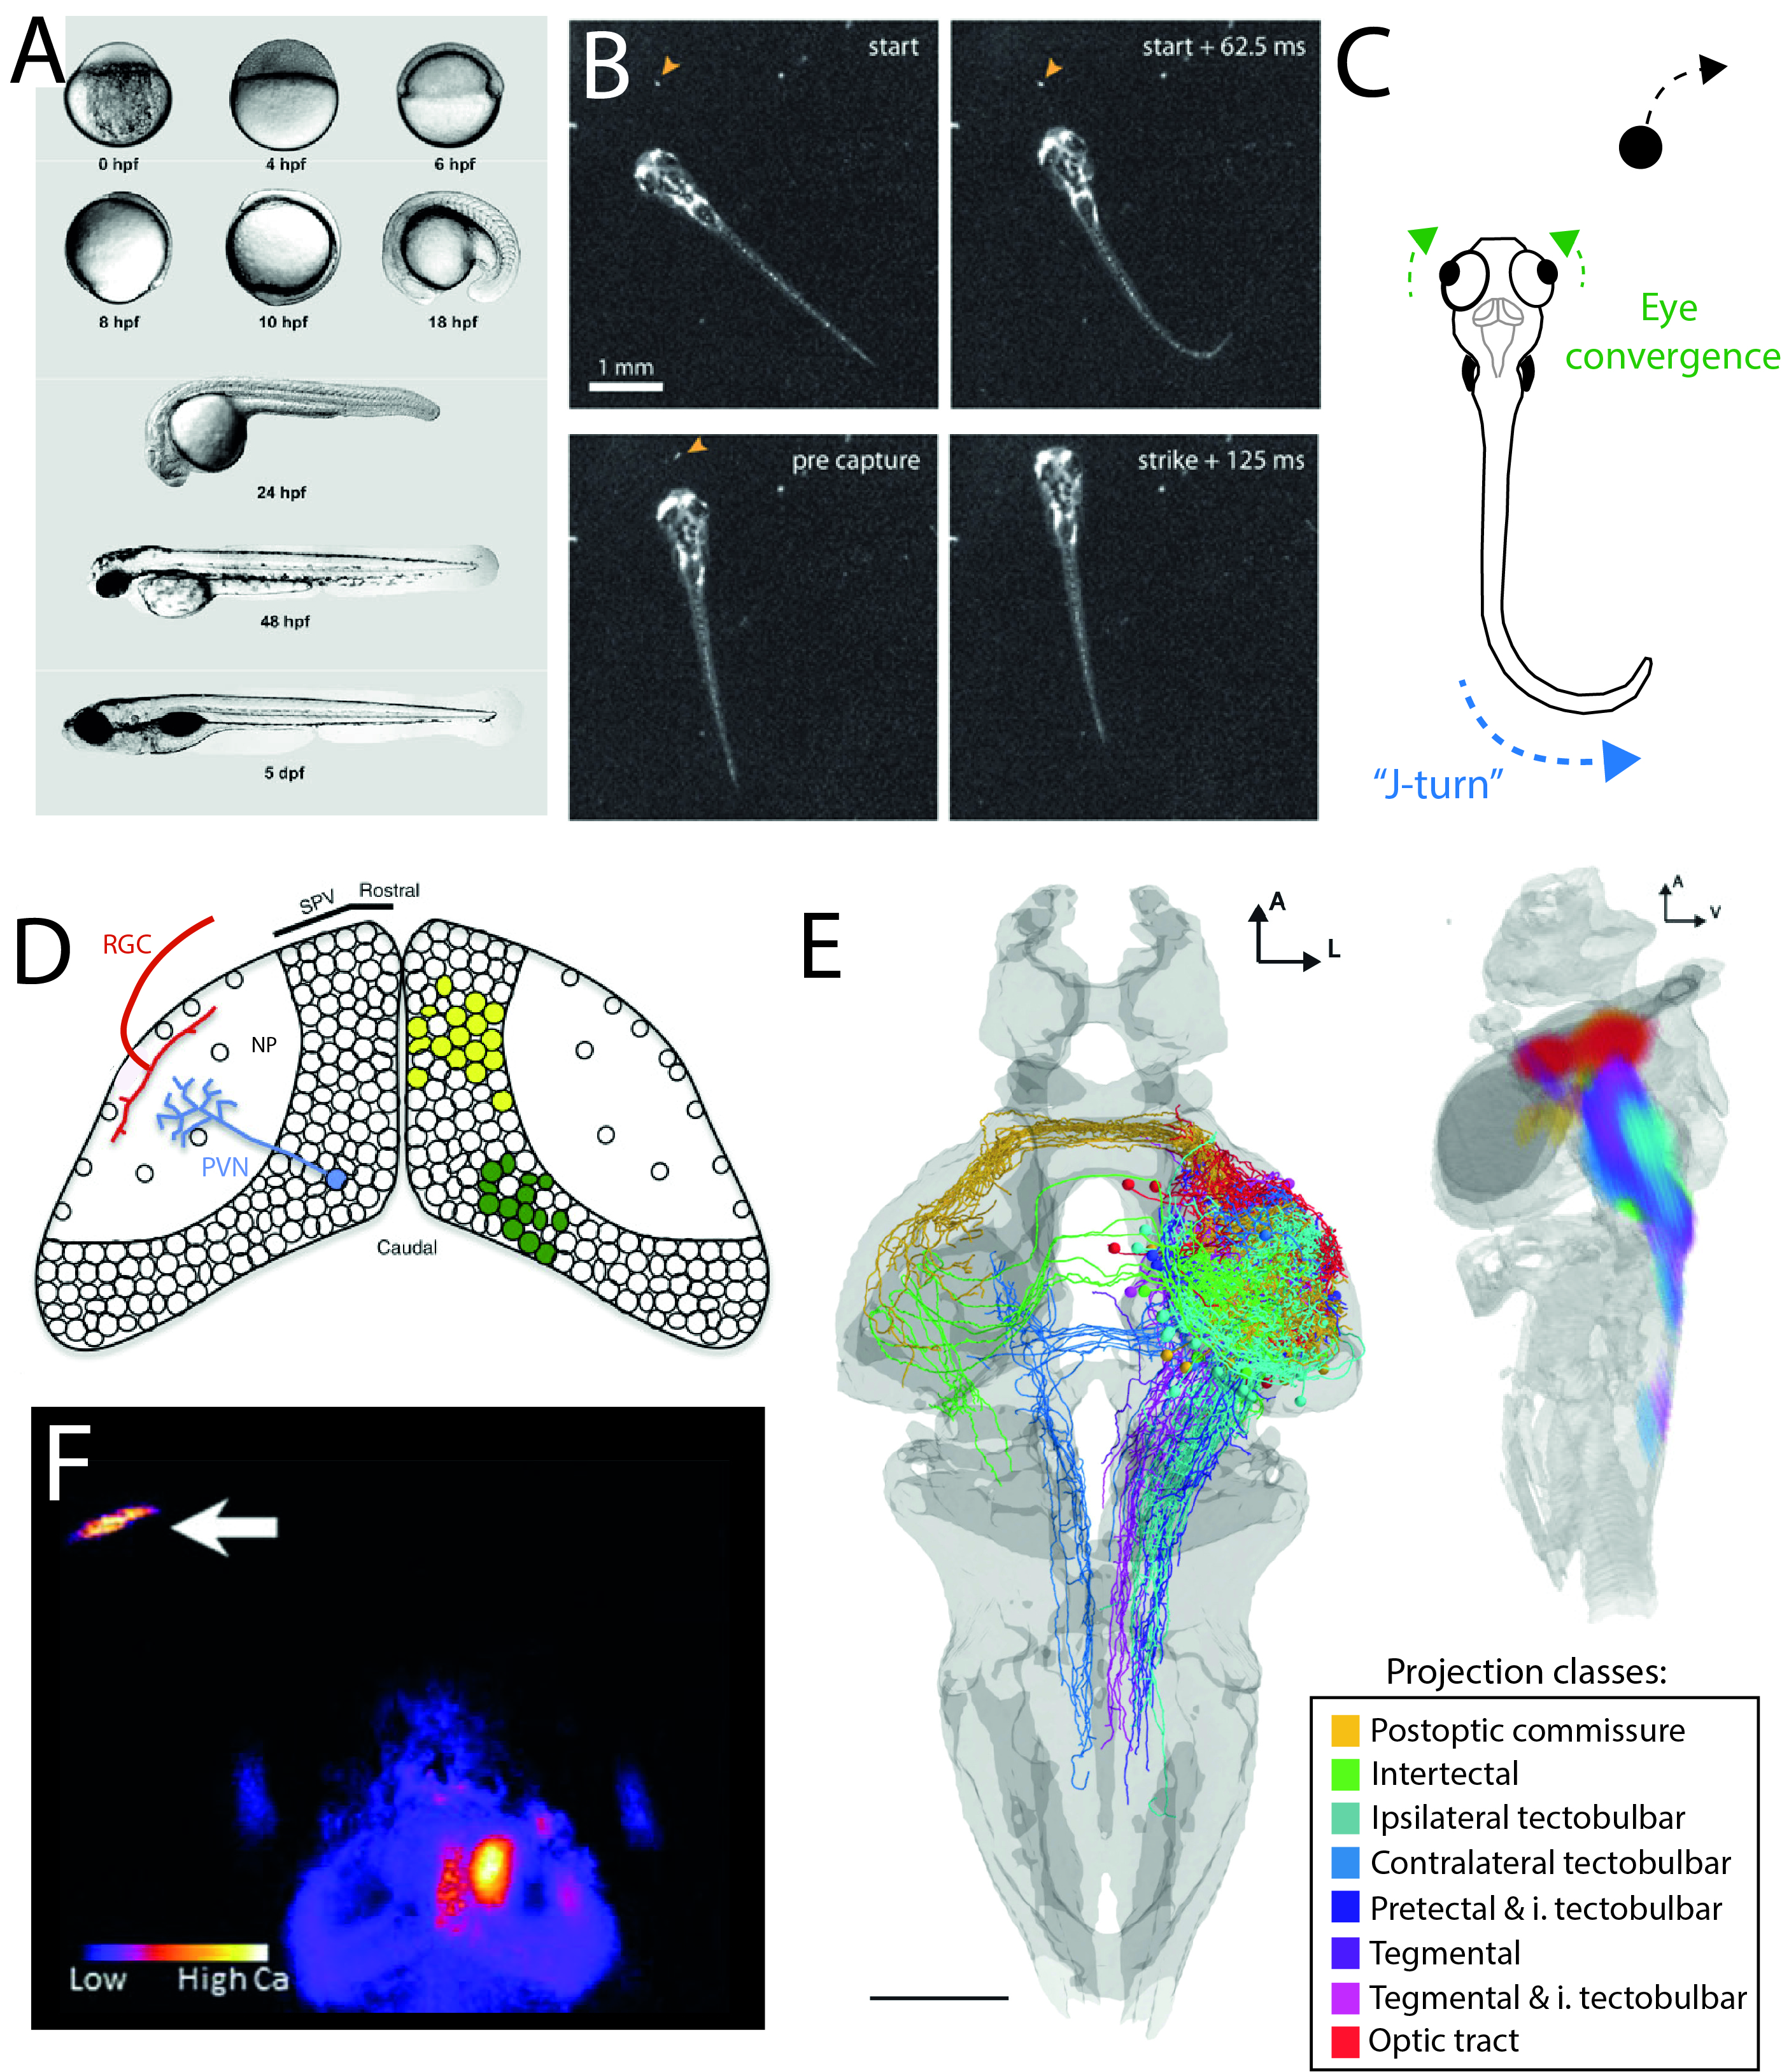
\includegraphics[width =  0.67\paperwidth]{Figures/I_Zebrafish_intro_v2.jpg}}
            \caption[\textbf{\label{fig:I_ZF}\textbf{Zebrafish as a model organism to study the effect of EE on visual behaviour and population activity in the tectum. }}]{ \textbf{\label{fig:I_ZF} zebrafish as a model organism to study the effect of EE on visual behaviour and population activity in the tectum.} \textbf{(A)} Zebrafish have a rapid external development. They go from a single cell (0 hours post fertilization - hpf) to a recognisable fish that is capable of generating visually driven behaviours in 5 days. \textbf{(B)} Frames from a movie of a zebrafish hunting down its prey (in this case a paramecium) which is marked by the orange arrow tip. Images from (\cite{Bianco2011}) \textbf{(C)} Schematic illustrating that during prey capture larval zebrafish converge their eyes and make “J-turns”. These turns, through a unilateral bend of the tail tip, orientate the fish towards the prey. Such movements are characteristic of prey capture, allowing for it to be distinguished from other behaviours. \textbf{(D)}  Schematic of tectal organisation to illustrate that incoming RGCs from the contralateral eye terminate in the tectal neuropil (NP). PVN cells (blue), with their cell body in the SPV extend their dendrites into the NP where they receive incoming sensory input. Many PVN neurons are organised into tectal assemblies (represented by the groups of neurons in green and yellow), which have been found to be active spontaneously and under visually evoked conditions. \textbf{(E)} A map of tectal efferents with both dorsal (left) and lateral views (right). Efferents are colored according to their projection class (bottom right table). Tectal effects project to multiple different motor targets in the tegmental midbrain and hindbrain (tectobulbar projections) in both ipsi- and contralateral projections. These are thought to be important for directing visually driven behaviours. Image from (\cite{Helmbrecht2018}). \textbf{(F)} A widefield image of a head fixed zebrafish expressing a calcium indicator in its optic tectum. The arrow points to a paramecium which is seen by the left eye causing a corresponding activation of tectal neurons in the contralateral tectal hemisphere. Image from (\cite{Muto2013PreyFunctions}).


        }
      \end{figure}

\clearpage

\subsection{Thesis Aims}
This thesis aims to understand how visual experience, in the form of naturalistic EE, influences the development of the visual system by using the larval zebrafish as a model organism.  The main biological questions to be addressed are: How does EE shape visually driven behaviour? Does EE shape developing tectal activity? and if so, what aspects of plasticity are important for these changes to occur? Finally, and perhaps most importantly, how do changes in tectal population activity development relate to changes in behaviour? These questions have been addressed through the following three results chapters:

\begin{enumerate}
    \item Prior to answering these questions it is important to be able to reliably describe the structure and dynamics of developing population activity. Therefore a recently developed bayesian inference method was applied to spontaneous activity in the tectum to give probabilistic estimates of neural assembly number, membership and dynamics (\textbf{Chapter 3}).
    
    \item To understand the effect of EE on visual system development zebrafish were raised in enriched environments (over a bed of gravel) or under normal laboratory conditions. The effect of this manipulation on behaviour was studied by examining how the prey consumption differed between these two rearing conditions. Following this, the development of spontaneously active neural assemblies was monitored to understand both how tectal functional connectivity was impacted by the visual environment and at what point in development these changes occurred. To examine the role of Hebbian plasticity and NMDAR subunit composition in facilitating experience-dependent effects in the tectum the effect of EE was studied in a novel zebrafish mutant. This mutant was a double KO of both paralogs of the genes encoding the NR2A receptor (\textit{grin2aa} and \textit{grin2ab}), a subunit that is known to shape plasticity in the mammalian brain (\textbf{Chapter 4}).
    
    \item Finally, to relate changes in population activity to hunting performance a “virtual reality” hunting assay was developed. This experiment setup allows for the visually evoked neural activity in the tectum to be monitored alongside tail movements while prey-like stimuli are presented. Decoding the position of these prey-like stimuli from tectal activity allows for the sensory representation of stimulus location to be investigated (\textbf{Chapter 5}). This provides an experimental setup that will be important for relating the effects of EE on the development of the tectum to changes in behaviour in future experiments. 
    
\end{enumerate}


   
   \chapter{Materials and Methods}
   \section{Zebrafish lines}
Calcium imaging experiments were carried out in zebrafish expressed \textit{Tg(HuC:H2B-GCaMP6s)} (Ahrens lab, Janelia farm). In this line, the \textit{HuC} promoter drives pan-neuronal expression of nuclear localised \textit{GCaMP6s} (these fish will be referred to as \textit{nls-GCaMP6s}). In addition,  \textit{nls-GCaMP6s} zebrafish that were null for genes encoding two isoforms of the NR2A subunit of the NMDAR (\textit{grin2aa -/-; grin2ab -/-}) were also imaged, this line will be referred to as the \textit{grin2a} \gls{dko}. To maximize optical clarity for imaging these fish were also compound \textit{roy;nacre} double homozygous mutants (\textit{casper}) larvae which lack melanocyte and iridophore pigmentation (\cite{White2008}). Behavioural experiments were performed using wild type (WT AB) fish generated by the mass embryo production service provided by the King's College London fish facility.

All larvae were raised at 28.5°C in Danieau solution (58mM NaCl, 0.7 mM KCl, 0.4 mM MgSO4, 0.6 mM Ca(NO3)2, 5 mM HEPES, pH 7.6) and were exposed to a 14 hour ON/10 hour OFF light/dark cycle. Larvae were fed daily from 5 \gls{dpf} using live rotifiers.  This work was approved by the local Animal Care and Use Committee (King’s College London), and was carried out in accordance with the Animals (Experimental Procedures) Act, 1986, under license from the United Kingdom Home Office.

\section{Generating the \textit{grin2a} double knock out in the \emph{nls-GCaMP6s} background}
\subsection{Breeding crosses}
Zebrafish posses two genetic paralogs encoding the NR2A subunit known as \textit{grin2aa} and \textit{grin2ab}. To create a DKO of the NR2A NMDAR subunit, both paralogs were targeted by \glspl{talen} that were designed to recognise start of exon 1, resulting in double strand breaks.  This caused a frame shift in both genes leading to a premature stop codon and a predicted truncated protein. This line was initially generated by Dr Paul Hunter in the \textit{HuC:GCaMP5} background, in which GCaMP is cytosolic. To compare functional imaging data in these mutants with fish expressing \emph{nls-GCaMP6s} this \gls{dko} needed be crossed with the \emph{nls-GCaMP6s} transgenic. To this end, \textit{grin2aa$_{(-/-)}$; grin2ab$_{(-/-)}$; HuC:GCaMP5$_{(-/+)}$} fish were out crossed with \gls{wt} fish containing no fluorescent reporter and their offspring screened for  non-fluorescence. The resulting \textit{grin2aa$_{(-/+)}$; grin2ab$_{(-/+)}$;  HuC:GCaMP5$_{(-/-)}$}  fish were incrossed and their offspring were genotyped by sequencing exon 1 to identify fish that were homozygous null for both \textit{grin2a} genes. These were then out crossed to the \emph{nls-GCaMP6s} line and their offspring incrossed. The resulting offspring were repeatedly incrossed until offspring expressed high levels of GCaMP fluorescence and were homozygous null for both \textit{grin2a} mutations  (\textit{grin2aa$_{(-/-)}$; grin2ab$_{(-/-)}$; nls-GCaMP6s $_{(+/+)}$}). 

\subsection{Genotyping}
For genotyping, adult suspected Grin2a mutants were temporarily anaesthetised in 0.025\% MS-222 (Sigma-Aldrich, catalog number: 886-86-2) in system water, and small tail samples were obtained. These samples were lysed in eppendorf tubes containing an alkaline buffer (25 mM NaOH; 0.2 EDTA) at 95$^{\circ}$C for 20 minutes. Each of the \textit{grin2a} genes were then amplified by \gls{pcr}. The PCR mix contained 12.5 $\mu$L platinum Hot start PCR 2x master mix, 0.5 $\mu$L forward primer (10 $\mu$M), 0.5 $\mu$L reverse primer (10  $\mu$M), 2 $\mu$L of genomic DNA and 9.5 $\mu$L nuclease free water. The PCR was run for 40 cycles with an annealing temperature of 58$^{\circ}$C. To ensure that DNA was amplified 5 $\mu$L of PCR product was run on a gel, and following the presence of a $\sim$450 bp band, was purified and sent for sequencing (Source Bioscience, Cambridge UK). For the PCR and sequencing the primers were as follows:



\begin{itemize}
    \item \textit{grin2aa}:
    \begin{itemize}
        \item  forward primer: 5'-GCAGCAAGGAGCATTCAG-3'
        \item  reverse primer: 5'-CTCTGTCAGAGATGTAGCGAG-3'
        \item  forward sequencing primer: 5'-GTATGCAGCAAGGAGCATT-3'
    \end{itemize}
    \item \textit{grin2ab}:
    \begin{itemize}
        \item   forward primer: 5'-GAACAGAGCGCAATCCC3-3'
        \item   reverse primer: 5'-CCAGTCCATGCAGTCTCTG-3'
        \item  forward sequencing primer: 5'-TGAATCGGTGCATGCCAAG-3'
    \end{itemize}
\end{itemize}
 
 Homozygous mutants were identified as having sequences identical to those in (\textbf{Figure \ref{fig:R2_F5}}) whereas heterozygous fish had double peaks in the sequencing data after the mutation site.

\section{Rearing protocol: Environmental enrichment by gravel rearing}
To assess the impact of visual experience on the development of naturalistic behaviour and visual system development, zebrafish were raised in different visual environments. Under laboratory conditions embryonic zebrafish usually develop in a petri dish placed on a shelf within an incubator. These rearing conditions lack many of the natural features of that zebrafish in the wild would usually experience (\cite{Engeszer2007ZebrafishField}). Therefore zebrafish were either raised under typical lab conditions (normally reared - \acrshort{nr}) or the petri dish rested on a bed of gravel (gravel reared - \acrshort{gr}). Gravel rearing the fish adds many of natural visual features that are lacking from the NR condition, creating an enriched environment. Gravel rearing started was started from 0-1 \gls{dpf}, before \glspl{rgc} begin to innervate the tectum at 2-3 \gls{dpf} (\cite{Burrill1994DevelopmentRerio}). Both conditions were fed rotifers (live prey) daily from the evening of 4 \gls{dpf} onwards.

\section{Functional imaging of spontaneous and visual evoked activity}
\subsection{Volumetric 2-photon calcium imaging}
To record neural activity in the tectum zebrafish of either sex were mounted in 2\% low melting point agarose in Danieau water with their dorsal side facing up on a custom built imaging slide and were submerged in Danieau water. These fish were left for 1 hour in the light so that the fish could settle, reducing drift while imaging. Neural activity was monitored by imaging the calcium dynamics of between 4000-6000  neurons in both tectal hemispheres with a custom built 2-photon microscope (Independent NeuroScience Services). Excitation was provided by a Mai Tai HP ultrafast Ti:Sapphire laser (Spectraphysics) tuned to 940nm. Laser power at the objective was kept below 15 mW for all fish. Emitted light was collected by a 16x, 1 NA water immersion objective (Nikon) and detected using a gallium arsenide phosphide detector (ThorLabs). Images (256 x 256 pixels) were acquired at a frame rate of 60Hz by scanning the laser in the x-axis with a resonant scanner and in the y-axis by a galvo-mirror. To enhance signal-to-noise every 2 frames for each focal plane were averaged. The focal plane was adjusted in 15$\mu$m steps using a piezo lens holder (Physik Instrumente). This allowed for volumetric data consisting of 5 focal planes to be collected at a volume rate of 4.8Hz. Scanning and image acquisition were controlled by Scanimage Software (Vidrio Technologies).

\subsection{Recording and analysis of spontaneous tectal activity}
To record spontaneous activity from the optic tectum mounted fish were placed in total darkness and volumetric calcium imaging was performed. To reduce transient neural activity that may be induced by the transition into this environment fish were allowed to adjust to the total darkness for $\sim$ 40 mins. To look at the development of spontaneous activity fish from 3, 5, 7 \gls{dpf} were imaged. All imaging experiments were conducted at 7 dpf.


\clearpage
\subsubsection{Preprocessing}
\newline
{\medium \textit{Image registration}\par}
Any recordings that showed drift in the z-plane were discarded. All other recordings where corrected for x and y drift by aligning every frame of the movie to the first image. This registration was performed using a nonrigid body alignment algorithm contained within the SPM8 plugin for MATLAB (\textcolor{blue}{http://www.fil.ion.ucl.ac.uk/spm/software/spm8}). Whilst this alignment corrected for slow drift of the fish caused by the agarose it could not correct for high velocity movements generated by the fish attempting to swim. This movement exceeds the
scanning rate of the microscope causing shearing of the image. As a result these frames were unusable and were manually removed.

\newline
{\medium \textit{Cell segmentation}\par}
Unlike cytosolyic GCaMP, the \emph{nls-GCaMP6s} line labels neurons in way that gives minimal overlap between neighbouring cells, reducing the likelihood of individual pixels containing mixed signals. Uniform expression within the nucleus results in an image that can be readily segmented, allowing for the detection of regions of interest corresponding to each neuron. Segmentation was performed on an average projection of the movie that had been smoothed with a 2D guassian kernel using a custom C++ script written by Giovanni Diana, Meyer Lab (\cite{Diana2019BayesianAssemblies}). Due to low pixel resolution within the images this segmentation algorithm takes into account both the morphology of the nucleus and the correlation of pixels within a segment, resulting in segmentation of cells that are active in nearly all cases. This produces a mask of labels that can be used to extract the time series for each neuron by averaging together all pixels with the same segmentation label for each frame of the movie. This has two distinct advantages over pixel wise analysis:
1) the traces for each neuron are less noisy than single pixels and 2) the number of
time series are reduced from 262144 x 5 pixels to  $\sim$ ~1500-3500 neurons, reducing the
computational load for subsequent analysis.

{\medium \textit{Detecting neuronal firing events from the fluorescence trace.}\par}
Raw fluorescence traces are built from a composite of signal from the calcium probe, low frequency fluctuations in baseline fluorescence (caused by bleaching of the calcium probe and z axial drift) and high frequency imaging noise.  Therefore, to quantify properties of neural responses the signal needed to be decomposed and the calcium signal extracted.
Furthermore, the decay of the GCaMP6s response is slow and is thought to be even slower when localized to the nucleus (\cite{Chen2013, Vladimirov2014}). This is likely to cause artefactual correlations. For example, two neurons firing a few seconds apart would appear to be correlated due to the slow kinetics of the probe. Therefore to examine temporal correlations, or the identify of neural assemblies (defined as synchronous groups of neurons), the time frames where neurons were most likely to be active needed to be inferred independently from the slow decay of the calcium probe.

For this purpose calcium signals were separated from baseline activity by using a a custom built R script, writtern by Giovanni Dianna, Meyer Lab (\cite{Diana2019BayesianAssemblies}). Briefly, this algorithm implements a \gls{hmm} to decompose the raw fluorescence into 1) the neuron activity state $S_{t}$ at time $t$ which is drawn from a Bernoulli process, 2) the background $B_{t}$ which is a Gaussian Markov process and 3) the imaging noise which is drawn from a Gaussian distribution.  Calcium signals are drawn from a normal distribution when the neuron activity state $S_{t}$ = 1 and follows an exponential decay when $S_{t}$ = 0. The values with maximum likelihood are then calculated conditional to the previous time points.  This processing gives both a calcium signal where noise and drifting baseline are absent and a binarised trace where a 1 represent a timepoint that the neuron was active and 0 when it is inactive. It is important to note that this binarised trace is not equivalent to actual spikes (action potentials), instead, it represents time points where there is maximum likelihood of the neuron being active. The calcium trace is subsequently used to calculate single neurons response properties such as response amplitude and duration whereas the binarised trace was used for correlations and identification of neural assemblies.

\subsubsection{Bayesian inference of neural assemblies}

Identification of spontaneously active neural assemblies in the optic tectum was achieved by using a Bayesian inference method called BINA (this method is explained in more detail in \textbf{Chapter 3} but for a full description see \cite{Diana2019BayesianAssemblies}). This method used a custom built C++ script, developed by Giovanni Dianna, Meyer Lab. In this method, a generative hierarchical model of synchronous activity is used to describe the organization of neurons into assemblies. Using Bayesian inference to infer the parameters of this model, this method provides a simultaneous estimation of assembly composition and within-assembly statistical features, such as the levels of activity, noise and assembly synchrony. 

The time taken to run this method is strongly influenced by the size of the activity matrix (neurons x frames) and the spontaneous activity recordings contained thousands of timepoints where few/no neurons firing. Therefore to speed computation times only frames with synchronous activity in more than 15 cells were used. For all recordings this threshold was used to select for synchronous activity events that had low probability (p < 0.02) of being random. This reduced compute times from over a week to 12-24hrs per dataset.

To approximate the probability distributions over the models parameters, BINA obtains samples using a Markov Chain Monte Carlo method known as a Gibbs sampler. This sampler randomly "walks" around the parameter space, preferentially sampling values which have higher probabilities. Since the Gibbs sampler initialises with random values, it takes a number of iterations before the sampler convergences on the posterior probability distribution. This convergence point could be identified looking by plotting log likelihood for each sample and observing a stable trace. Convergence was typically reached after 400,000 samples therefore each dataset was run for 600,000 samples, ensuring that convergence was definitely reached. The last 200 of these samples were then used as an approximation of the posterior probability distributions for each of the parameters. Neurons that could be assigned to an assembly in 99\% of these samples were treated as neurons that could be assigned to a single assembly. 

Metrics quantifying the structure and dynamics of the assemblies either utilised the model parameters directly or were calculated from them. All assembly metrics are explained throughout the results chapters. All statistical analysis of neural assemblies parameters across development and between genotypes were analysed in R. All statistical tests are reported throughout the chapters as they are used.

\subsubsection{Identifying correlated sub-networks of tectal assemblies}

To look at the organisation of correlated activity between tectal assemblies, pair-wise correlations were calculated between each assembly pair using the inferred time series of assembly activations that were inferred using the BINA method and this process was repeated for each sample of the posterior. A graph describing the assembly correlation was then constructed by adding a edge between all assembly pairs which has a positive correlation in over 95\% of the samples. This graph could then be clustered into subnetworks of correlated assemblies using the Girvan-Newman method (\cite{Newman2004FindingNetworks}) as implemented in the igraph R package (\cite{Csardi2006TheResearch}).


\subsection{The virtual reality hunting assay: visually evoked activity and behaviour}
\subsubsection{Imaging setup}
In order to simultaneously image visually evoked activity in the tectum and  tail movements 7 \gls{dpf} zebrafish were mounted in 2\% agarose within a custom built perspex cylindrical chamber. The fish was positioned so that its right eye faced a semi-circular screen covered in a grey diffusive filter and the chamber was filled with Danieau solution. This screen occupied 153$^{\circ}$ X 97$^{\circ}$ of visual space in terms of azimuth and elevation and was positioned 20 mm away from the fish. Visual stimuli could then be projected onto this screen using a P2JR pico-projector (AAXA Tech). To avoid interference of the projected image with the signal collected by the detector, a red long-pass filter (Zeiss LP590 filter) was placed in front of the projector. In order to image the fishes tail movement the imaging chamber was placed in the center of a 3D-printed semicircular ring of infrared LEDs. The infrared light hitting the fish body was refracted and reflected downwards, through the clear bottom of the chamber, onto a hot mirror which in turn reflected the light into Chameleon 3 FLIR camera imaging at 400Hz. This camera was fitted with a shortpass 900nm filter which allowed infrared light to pass through while blocking light from the laser. The camera, microscope and visual stimulation were synchronised via a transistor-transistor logic pulse that was sent from the microscope on the first frame of image acquisition. In this setup the visual evoked activity in the fish tectum could be imaged by volumetic calcium imaging (as above) while tail movements were monitored by the camera below for 1 hr. 

\subsubsection{Visual stimuli}
Visual stimuli were generated using a custom C$^{++}$ script written by Giovanni Dianna, Meyer lab.  5$^{\circ}$ black spots were presented at three different locations in visual azimuth separated by 10$^{\circ}$ intervals (-10$^{\circ}$, 0$^{\circ}$, +10$^{\circ}$). 0$^{\circ}$ was defined as the center of the screen, orthogonal to the zebrafish body axis. These spots moved with motion that resembled rotifer movement within a neighbourhood (5$^{\circ}$ radius) at a speed of 30 degrees/sec. These stimulus parameters were selected because they have been shown to induce hunting behaviours in head fixed larval zebrafish.

These dots were presented in two blocks which differed in the background they were projected over. In one block the background was a picture of gravel and the other it was simply a grey screen (\textbf{figure \ref{fig:m1}A}). Both backgrounds were presented in monochrome meaning that they did not differ in their color spectrum. In these blocks each spot was presented a total of 17 times per block in 5 second epochs, followed by 40 seconds of black screen. Importantly the movement of the dot was identical in each presentation Both the order of the blocks and order of these spots within the blocks were pseudo-randomised. Often fish can become startled by the initial stimulus. Therefore the fish were presented with a additional epoch, consisting of concentric rings moving inwards to a central point, prior to the experimental blocks. Furthermore, both the background and the dots faded in and out over the course of half a second to minimise any startle effects but that may be caused by sudden changes in the stimulus.

To understand what features of the background may be causing any changes in activity between these two blocks certain visual features were calculated to understand differences between the two backgrounds more fully. Firstly, contrast has been shown to be important for the detection of prey (\cite{Bianco2011}) with hunting behaviours being more likely to be initiated at greater contrasts therefore the mean difference in luminance between the background and the prey-like dots was calculated. This showed that the textured background had less contrast between the stimuli and background when compeared to the the grey background (\textbf{figure \ref{fig:m1}B}). However, the textured background has lots of local variance in luminance which could create high localised contrast between the stimulus and background. Therefore the difference between each pixel in the background and the stimulus was calculated. This showed that all pixel wise local contrast was less in the textured background, this should make it more difficult for the fish to detect the prey against the textured background. In addition, the power spectrum of difference spatial frequencies in the two backgrounds was calculated. The grey background, unsurprisingly had no different spatial frequencies. The textured background on the other had showed a wide range of different spatial frequencies, and resembled distributions that are typical of natural scenes (\cite{VanderSchaaf1996ModellingInformation}). Therefore it is possible that the differences in visually evoked activity between the two blocks may be driven by these differences in spatial frequencies between the two backgrounds as all other stimulus features are constant and differences in contrast are greater in the grey background.




\begin{figure}[!htb]
        \center{\includegraphics[width = 0.8\paperwidth]{Figures/m1.pdf}}
        \caption[\label{m1} \textbf{The difference in the statistics of the background between the two presented stimuli.}]{\label{fig:m1} \textbf{The difference in the statistics of the background between the two presented stimuli.  (A)} Two images showing a 5 deg spot being presented either over a grey background or a textured background. These stimuli were projected onto a curved screen positioned in front of the fishes eye \textbf{(B)} A histogram showing the change in luminance between the black dot and the background. The grey bins indicate the distribution of localised differences in luminance between the stimulus and pixels within the textured background. The green dotted line shows the the mean difference between the textured background and stimulus. The red line shows the difference in luminance between the grey background and the stimulus.  \textbf{(C)} Matrices showing the distribution of spatial frequencies in each background. \textbf{(D)} Power spectral density plot of the spatial frequencies shown in C. Only the textured background has been plotted as no spatial frequency changes were present in the grey background.}
      \end{figure}

\subsubsection{Preprocessing of visual evoked neural activity}
All data obtained from the virtual reality hunting assay was analysed using a custom written Python script. Visually evoked functional imaging data was both aligned and segemented using the Suite2p Python package (\textcolor{blue}{https://mouseland.github.io/suite2p}, \cite{Pachitariu2016Suite2p:Microscopy}).  The fluorescence level can vary between cells and change over the course of imaging due to bleaching and drift. Therefore the raw fluorescence for each cell, $F(t)$, was  normalised by calculating the $\Delta F/F(t)$ for each time $t$. This was defined as:

\begin{equation}
    \frac{\Delta F}{F} = \frac{(F(t) - F_{0}(t))}{F_{0}(t)}
\end{equation}

Where $F_{0}$ is the fluctuating baseline fluorescence that was estimated by calculating the bottom 8$^{th}$ percentile of groups of frames using a sliding window of 400 frames and was then smoothed with a Gaussian kernel.  This gave a smooth baseline that was fitted to timepoints that were unlikely to be calcium events. 

Many normalised traces were found to contain no calcium events over the time course of imaging. These inactive cells were removed using a "min-max" procedure. In this procedure a sliding window smaller than the typical duration of a calcium event (5 frames) was rolled through the $\Delta F/F$, calculating the minima for each window. The maxima of these minima were then calculated for each trace. This allowed for active traces to be identified because if the window encountered a calcium event the maxmin would be high, due to the sustained deviation from baseline, whereas inactive traces that fluctuated around baseline would have a low maxmin. As a result, a maxmin threshold of 0.1 $\Delta F/F$ was found to distinguish between active and inactive cells in all imaged fish (as determined by visual inspection of the traces). Of these only a subset of neurons were found to be responding to the stimulus.

Some neurons, likely to be related to ongoing activity or behaviour, may negatively impact decoding performance because their activity is sporadic, creating noise for the decoder (\cite{Kahn2015ANeurons}). In order to assess the impact of these cells on decoding performance we distinguished neurons that were responding to the stimulus by comparing the activity of neurons to that of random noise model for each neuron. To do this neuron traces were first binarised by setting timepoints exceeding 2 standard deviations of the mean for each trace to 1 and all other timepoints to  0. If $x_{i}$ represents the activity state of the neurons at each time $i$, $s_{i}$ denotes whether a stimulus is being shown ($s_{i}$ = 1 if stimulus is being presented or $s_{i}$ = 0 if stimulus is not being presented) and N represents the number of frames, then a \gls{ncc} can be calculated for each neuron by:

\begin{equation}
    NCC = \frac{1}{N} \sum_{t = 1}^{N}s_{i}x_{i}
\end{equation}

A neuron that reliably responds to every frame that there is a stimulus presentation would therefore have a NCC = 1, whereas one that is only  active at times when no stimulus is presented would have an NCC = -1. To identify neurons that were not firing in response to the stimulus (ie. firing randomly) the NCC value for each neuron was compeared to the average NCC for its own random noise model. To do this the expected value of the NCC ($\langle NCC \rangle$) for each neuron was calculated as if it was firing randomly with the same firing probability. A neuron was identified as visually responsive if its NCC value exceeded three standard deviations of the $\langle NCC \rangle$ of its own random noise model. This gives a threshold for being visually responsive for each neuron whilst taking into account its own firing probability. 
 
\subsubsection{Decoding}
In order to decode stimulus identity from neural activity the mean response for each neuron ($N$) to each stimulus presentation ($E$) was calculated to give a $N$ X $E$ stimulus response matrix. Here each column represents the population response over all neurons for a single stimulus presentation. A separate vector of length $E$ contained labels corresponding to the stimulus that had caused each population response.
These could be used to train the decoder to predict the stimulus identity from the population response. 

Decoding was performed using two separate linear decoders, \gls{lda} and \gls{logreg} (for more details see \textbf{Chapter 4}). Both decoders were trained using a leave-one-out cross validation strategy,  where a single population vector and it's corresponding label were removed from the training data set for testing. This leave-one-out procedure was repeated for all population vectors and the decoding performance was measured as the percentage of correctly decoded classes. All cross-validation and decoding steps were implemented in Python using the scikit learn library (\textcolor{blue}{https://scikit-learn.org/}).


\subsubsection{Tracking of tail movement and analysis}
The tail was tracked from behavioural recordings using \gls{dlc}, a \gls{cnn} designed for behavioural tracking (\cite{Mathis2018DeepLabCut:Learning}). This CNN uses a Resnet50 architecture that had been pretrained on tens of thousands of natural images (ImageNet database). Added downstream of this architecture are distinct readout (deconvolutional) layers which predict the probability that a labeled body part is in a particular pixel within the image. By initialising with pretrained weights DLC is able to transfer this learning to the tracking task, yielding highly accurate estimates of body position from small training datasets and with fast training times (\cite{Mathis2018DeepLabCut:Learning}; \cite{Mathis2020DeepNeuroscience}). 

In order to train this network, 250 frames from 3 different tail recordings of spontaneous tail movement were selected for labeling, these contained a variety of images of the tail at different phases of movement. For each of these frames eight positions along the tail were manually labeled, these positions were: the center of the fish's body (swim bladder), its tail tip and 6 evenly spaced locations between them. The \gls{cnn} was then trained on 200 frames of this labeled dataset for 250,000 iterations ($\sim$2 hours, Google Colab GPU). The remaining 50 labeled frames were used as a test set to assess the accuracy of the model. Test label prediction error was < 8 pixels, this was less than the width of the tail in the image ($\sim$13 pixels) and was therefore deemed acceptable. 

To calculate the tail angle at each timepoint of the movie the labeled points were skeletonised by treating the regions between the markers as separate vectors (or bones). The angle between each of these vectors relative to the x-axis was calculated. This was then subtracted from the average angle for each of these bones in the first 200 frames of the movie (prior to any movement of the tail). This gave the angle between the midline of the tail and each of the bones at each frame. The sum of these angles was then taken to give a trace that represented the total tail angle relative to the midline.

To automatically detect swim bouts, the first derivative of the total tail angle was calculated and was then smoothed with a Gaussian kernel of 20 frames. This had the effect of dilating neighbouring tail beats, creating a series of continuous positive values, which could then be binarised into segmented bouts using a threshold of 0.2 (arbitrary activity units). The peak of the first turn in each swim bout was used to calculate metrics of t. These quantified whether the turn fell within an epoch, its direction relative to the stimulus, it's latency relative to the epoch onset and tail angle.  


\section{Prey capture behavioural assay}
Hunting performance of zebrafish larvae was assessed using a hunting assay. For this assay rotifers were pipetted into 35mm petri dishes containing 3 ml of Danieau solution. These dishes were then placed within a custom built infrared LED ring (835nm) and and then imaged using a Chameleon 3 FLIR camera (30Hz) for 30 seconds. After this initial recording either GR or NR 7 \gls{dpf}  zebrafish larvae were added to the dish and were placed on either a gravel background or over a piece of white paper. The fish were then allowed to hunt over this background for 30 mins and then recorded again to assess how many rotifers the fish had consumed. Prior to recording both groups of fish were placed on the testing background for 40 mins to allow the fish to acclimatise to the novel visual background.

As some rotifers can be obscured by the side of the dish the 30 recordings were separated into 5 second segments and the mean count was taken. As the rotifers move around by swimming this ensured that rotifers who were at the side of the dish could be counted at other points in the movie. For these manual counts each frame in a segment was coloured in a different color and superimposed, this enabled rotifers to be distinguished from debris in the dish based on their swimming trajectory. All movies were assigned a random ID prior to counting using a custom built R script, blinding the counter to the experimental condition. Some group wise data from these experiments was non-normally distributed. Therefore group comparisons were analysed using pair wise Man-Whitney U-tests with Bonferroni corrections.
    
    \chapter{Population activity in the optic tectum of the larval zebrafish}
    \section{Introduction}
During the development of the visual system neurons must make precise synaptic connections with each other, producing neural circuits that are capable of generating visual guided behaviours. As these connections change, so too must the patterns of activity that are distributed across these populations of neurons.  A major goal of this thesis is to understand how the developmental trajectory of such population activity is influenced by changes in the visual environment because these changes are likely to underlie any changes in behaviour.  A prerequisite of this is that features of population activity can be quantified in order understand how the underlying neural circuitry maybe altered. Therefore the aim of this first results chapter is to introduce methods and metrics to quantify the structure and dynamics of population in the tectum. These methods will be used in subsequent chapters to understand how EE modifies the development of population activity in the tectum.

One approach to studying the circuit architecture of the visual system is to record activity when the organism is in total darkness. This is because high levels of activity persists and correlated activity is likely to be seen between neurons that share a high degree of connectivity with each other rather that being driven by a common source, such as a visual stimulus.  As a result, previous studies have shown that spontaneous activity takes the form of discrete local populations of neurons known as neural assemblies which show spatiotemporally orchestrated patterns of coactivity (\cite{Miller2014}; \cite{Carrillo-Reid2015}). Importantly these same assemblies that are spontaneously active have been shown to be active during natural vision and correlate with certain behaviours (\cite{Miller2014}; \cite{Carrillo-Reid2015};  \cite{Stringer2019SpontaneousActivity}; \cite{Luczak2007}; \cite{Romano2015}). These observation has led to the suggestion that neural assemblies may be acting as the functional units of the brain and that spontaneous activity, due to network constraints, revisits preferred network states through "attractor-like" dynamics (\cite{Hebb1949}; \cite{Romano2015}; \cite{Yuste2015}, \cite{Marachlian2018PrinciplesTectum}). Therefore the structure of spontaneous activity can give insight into the underlying patterns of functional connectivity within the visual system allowing for the developmental trajectory of circuits in the visual system to be mapped (\cite{Avitan2017}; \cite{Pietri2017}).

However, automatically identifying and quantifying features of assemblies from population recordings can be challenging for a number of reasons. Firstly, the number of assemblies is not known \textit{a priori}. Secondly, an assembly's constituent neurons are noisy with not all neurons being recruited at every assembly activation and some neurons may fire independently from their assembly. Assemblies also show temporal overlap in their firing, making them difficult to distinguish from each other. Finally, some neurons may not be tightly coupled to an assembly at all and therefore their activity generates noise when clustering (\cite{Molter2018}; \cite{Diana2019BayesianAssemblies}).

Previous methods to identify assemblies have either relied upon dimensionality reduction techniques such as \gls{pca} followed by factor analysis, or spectral clustering methods to identify communities from graphical representations of the data (\cite{Lopes-dos-Santos2011}; \cite{Carrillo-Reid2015}; \cite{Romano2015}; \cite{Avitan2017}).  These methods can perform well in scenarios where there are clearly defined independent groups and that fire with low levels of noise (\cite{Molter2018}). However, as the complexity and noise within the data increases these techniques can lead to spurious conclusions as shown by ground truth validation tests (\cite{Diana2019BayesianAssemblies}). Furthermore, as these methods do not quantify the certainty over the assignment of a neuron to an assembly there is no way of knowing when neurons are likely to be miss-assigned.  To address these problems a member of our lab recently developed a new method which utilises a hierarchical model of assembly activity and Bayesian inference techniques. This method (\gls{bina}) has been shown to out perform previous methods in validation tests, even in scenarios where the level of noise is high (\cite{Diana2019BayesianAssemblies}). Unlike other existing methods it also uses a statistical framework that provides probabilistic estimates of assembly number, membership and activity. Therefore this method could be used to understand both the structure and dynamics of assemblies within the developing brain.

The aim of this chapter is to characterise the structure of population activity in the optic tectum at 7 \gls{dpf} when a fish is raised under normal laboratory conditions. At this age the optic tectum already possesses the neural circuitry required to engage in complex visually guided behaviour such as prey capture (\cite{Gahtan2005}; \cite{Bianco2015}). Consistent with previous studies I find that spontaneous activity is characterised by groups of synchronously firing neural assemblies (\cite{Romano2015}; \cite{Avitan2017}; \cite{Pietri2017}). Using the Bayesian inference method to quantify both the structure and dynamics of these assemblies reveals that the majority of assemblies are spatially compact and lateralised and that assembly structure and organisation correlates with assembly dynamics. This chapter therefore provides a description of population activity in the tectum that can be used to understand how this tectal circuitry develops and is shaped by the visual environment in subsequent chapters.

\section{Results}
\subsection{Calcium imaging of spontaneous activity in the optic tectum}
To study the how spontaneous population activity is organised within the optic tectum 7 \gls{dpf} larval zebrafish expressing \textit{nls-GCaMP6s} under a pan-neuronal promotor were imaged for ~1 hr in complete darkness. This imaging was performed using 2-photon microscope equipped with a resonant scanner and peizo lens holder enabled fast volumetric imaging of both tectal hemispheres at a rate of 4.8Hz per volume (\textbf{Figure \ref{fig:R1_F1}A-C}). Each volume consisted of 5 optical sections that were approximately 15$\mu$m apart giving a total imaging depth of 75 $\mu$m covering 75\% of the tectal volume.  Following image acquisition each slice was registered to itself, the cell bodies were were segmented from the registered mean images and the fluorescence signal for each cell was extracted with around 3000-4000 cells being segmented per fish, although not all of these were active (\textbf{Figure \ref{fig:R1_F1}D}). 

Whilst the on rate of GCaMP6s is relatively fast, the decay of the response is slow and is thought to be even slower when localized to the nucleus (\cite{Chen2013}; \cite{Vladimirov2014}). This is likely to cause artifactual correlations between neurons if the complete extent of the GCaMP6s signal is used for correlation analysis. For example, two neurons firing a few seconds apart would appear to be correlated due to the slow kinetics of the probe. To avoid such a scenario a \gls{hmm} was used to binarise the trace by identifying timepoints where there is maximum likelihood of the neuron being active (\cite{Diana2019BayesianAssemblies}). It is important to note that the inferred events do not correspond to individual action potentials but timepoints where there is maximum likelihood of the neuron being activate. This can be used to identify correlations between neurons. In addition, this model can also reconstruct the calcium signal (free from signal noise and drifting baseline) so that parameters such response amplitude and duration can still be estimated \textbf{(see Figure \ref{fig:R1_F1}E and \textbf{Materials and methods})}. Any traces that contained no calcium events throughout the duration of the recording were discarded.

\begin{figure}[!ht]
        \center{\includegraphics[width =  0.8\paperwidth]{Figures/R1_F1.pdf}}
        \caption[\label{fig:R1_F1} \textbf{Recording spontaneous activity from the optic tectum of the larval zebrafish.}]{\label{fig:R1_F1} \textbf{Recording spontaneous activity from the optic tectum of the larval zebrafish. (A)} 7\gls{dpf}	 zebrafish	 larvae	 expressing	 \emph{nls-GCaMP6s}	 were	 mounted	 in agarose	 and	 the spontaneous	neural	activity from	both	tectal	hemispheres	was imaged in a	single	plane using	a	 two	photon	microscope	in	 total	darkness	 for	one	hour. \textbf{(B)} A high resolution single slice through the center of the zebrafish brain with pan-neuronal expression of \emph{nls-GCaMP6s}. The optic tectum is a large bilateral structure sitting on the dorsal surface of the mindbrain (highlighted in blue).  \textbf{(C)} Imaging volumes consisted of 5 optical slices that were 15$\mu$m apart and were imaged at 4.8Hz per volume. \textbf{(D)} A mean image of tectal cells in a single optical slice with active cells segmented (highlighted in blue). \textbf{(E)}  The raw fluorescence signal for each cell (black) was binarised into time points where there was maximum likelihood of the neurons being active (red) using a hidden Markov model. This model also allowed for the calcium signal to be reconstructed (green). }
      \end{figure}
    
\subsection{Single neuron properties of neurons within the tectum}
Prior to understanding the interactions between neurons I wanted to determine how the firing properties of single neurons within the tectum because these may be affected by  both development and visual experience (\cite{Pietri2017}; \cite{Avitan2016}; \cite{Pratt2007HomeostaticCircuit}). Firstly, the number of active cells in each recording were estimated from the segmentation. Around 400-500 cells were found to be active in each optical slice meaning that the number of active cells in each volume was approximately 2257$\pm$188 (mean $\pm$ \gls{sd}) \textbf{(Figure \ref{fig:R1_F2}A}). The segmentation algorithm identifies neurons based on both morphology and correlated activity between pixels. This means that it mainly active cells are segmented, making it difficult to assess what proportion of cells in the tectum are active. However, manual counting of a couple of optical slices provided estimates that between 50-70\% of cells were spontaneously active within our recordings. 

\begin{figure}[!htb]
        \center{\includegraphics[width = 0.7\paperwidth]{Figures/R1_F2.pdf}}
        \caption[\label{fig:R1_F2}  \textbf{Response properties of spontaneously active neurons.}]{\label{fig:R1_F2}  \textbf{Properties of spontaneous active neurons in the optic tectum. (A)} The number of active cells in the optic tectum of all fish (n=8). Density plots for single neuron properties such as \textbf{(B)} Firing frequency (events/second), \textbf{(C)} response amplitude  ($\Delta$F/F) and \textbf{(D)} response duration (seconds). For all density plots the grey lines demonstrate the distribution for each fish and the the purple line represent the mean distribution across fish.}
      \end{figure}


In order to understand the distribution of firing properties of these active neurons a number of activity parameters were calculated. Firstly, the firing frequency was calculated from the binarised trace by counting the average number of active time-points per second for each neuron. It should be noted that this is only a rough estimate of firing frequency as there are likely to be far more spikes within a single time frame. Each fish was found to have a very similar sparse levels of activity where found across all fish with he majority of data centered around a mean across fish of 0.06 $\pm$ 10$^{-5}$ events/second and a tail that extended towards higher frequencies \textbf{(Figure \ref{fig:R1_F2}B}). Finally, by isolating each response from the inferred calcium signal the mean response amplitude and duration for each neuron could be calculated \textbf{(Figure \ref{fig:R1_F2}C-D}). Here response amplitude and duration are likely to reflect frequency and length of the underlying spike trains. Like firing frequency, all fish showed similar distributions for both response amplitude and duration with a mean of  0.75$\pm$ 0.018 $\Delta$F/F and 4.90$\pm$0.18 Seconds respectively. 


\subsection{Spontaneous activity is correlated in groups of spatially clustered neurons}

Having looked at the properties of single neurons I next  determined the spatiotemporal organisation of population activity. To do this, cell activity was plotted by time in a raster plot and the number of neurons at each time point were summed revealing that there were frames with a high degree of synchronous activity (\cite{Romano2015}). In order to understand if this structure could be explained by chance the time series for each neuron was circularly permuted. This has the effect of breaking the temporal structure between neurons yet preserving the firing statistics for each neuron.	By totalling up the activity at each frame there were a large number of frames where the coactivity in the data exceed	95\% of	the	distribution seen in the circularly permuted data (\textbf{Figure \ref{fig:R1_F3}A}). Thus the degree of pairwise correlated activity is more than would be expected by chance (\textbf{Figure \ref{fig:R1_F3}B}).

Synchronous events could be random, or they could represent the repeated spontaneous activation of the same groups of neuron in assemblies. To investigate this, a \gls{mi} between each frame was computed (\cite{Romano2015}):

\begin{equation}
    MI = 2\frac{\left | A \bigcap B \right |}{\left |  A + B\right |}
\end{equation}

where a and b are binary population vectors indicating the active and inactive neurons in a timeframe (1 = active, 0 = inactive). This gives a measure of similarity between the two frames where 1 indicates that two frames have all of the same neurons active and 0 indicates none (\textbf{Figure \ref{fig:R1_F3}C}). Pairwise MI values between frames were used to generate a similarity matrix for both significantly synchronous and non-synchronous events. For synchronous events the similarity matrix displayed an off diagonal block-like structure. Moving across a row of the matrix it was clear that similar frames occurred at multiple different points within the recording (\textbf{Figure \ref{fig:R1_F3}D}). These repeating frames did not always align vertically with those of other rows suggesting different populations of neuron were active at different times.  Importantly, this block-like structure was greatly reduced for non-synchronous events. This indicates that there are multiple different discrete populations of neurons that fire together synchronously and repeatedly throughout the recordings. 

\begin{figure}[!htb]
        \center{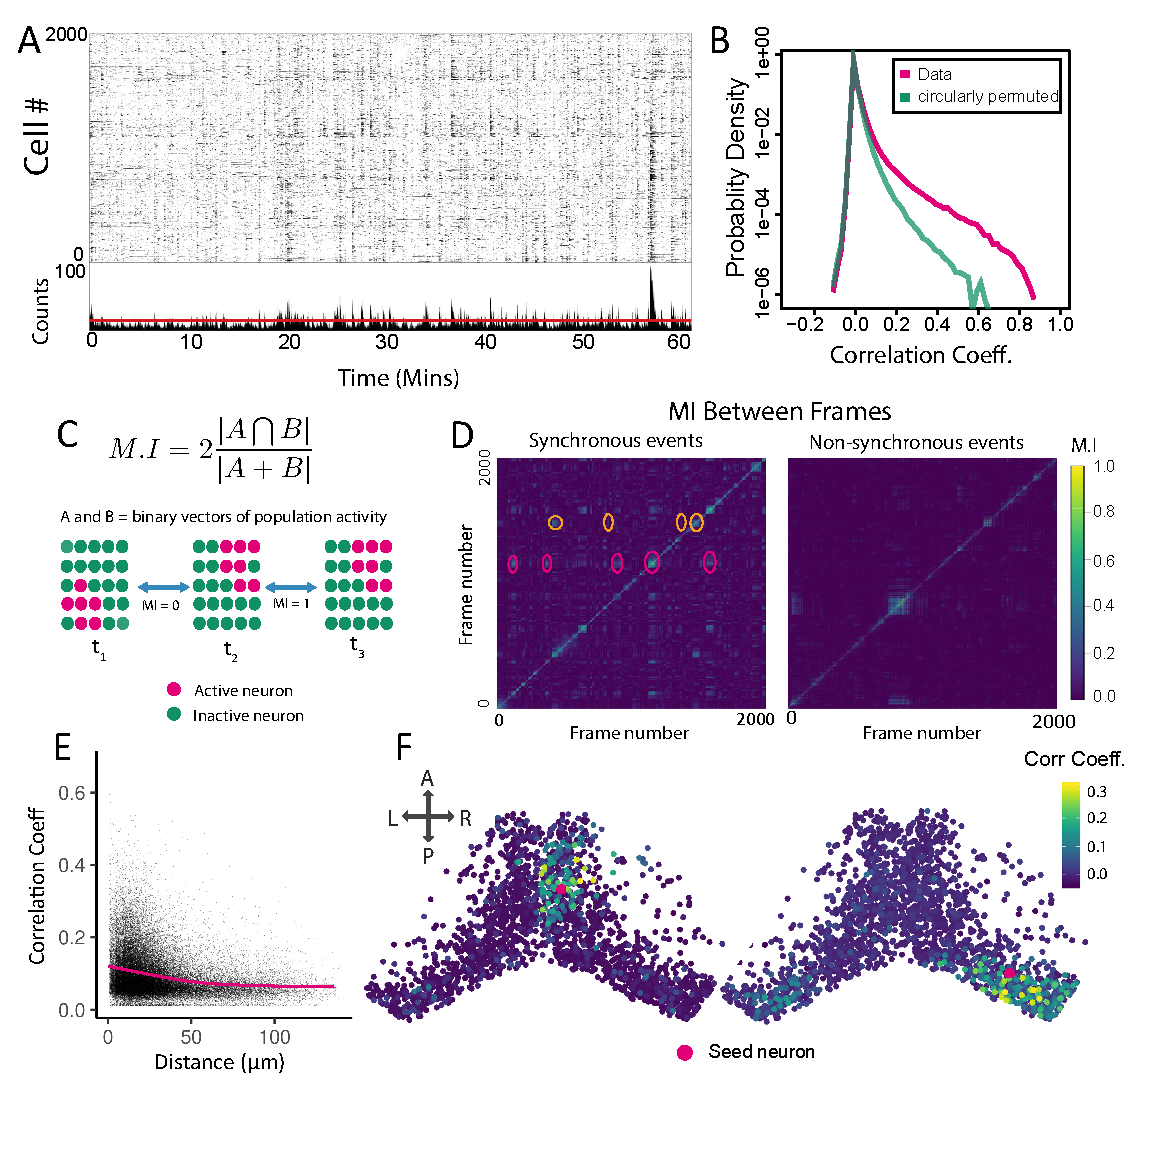
\includegraphics[width = 0.8\paperwidth]{Figures/R1_F3.pdf}}
        \caption[\label{fig:R1_F3} \textbf{Spatiotemporal organisation of spontaneous activity in the tectum.}]{\label{fig:R1_F3} \textbf{Spatiotemporal organisation of spontaneous activity in the tectum.  (A) Top:} Raster plot of population activity in the optic tectum. At certain time points the raster plot shows vertical banding, indicating that there is synchronous activity  across neurons. \textbf{Bottom:} The  number of cells that were active in each frame were counted. This shows frames where there are synchronous activation of cells which can not be explained by chance. The red line represents the 95\% of the distribution of coactive cells in a null model where the data was circularly permuted.  \textbf{(B)} The distribution of pairwise correlations in the tectum compared to the same null model as in A. \textbf{(C)} To understand if the same groups of neurons were repeatedly active throughout the recording, a \gls{mi} was calculated for all pairwise population vectors (ie. neurons active in each frame). This index ranged from 0 (no neurons in common - $t_{1} \ vs \ t_{2}$) to 1 (all neurons in common - $t_{2} \ vs \ t_{3}$). Where $t_{n}$ is a timeframe containing active and inactive neurons. \textbf{(D)} similarity matrices for synchronous and non-synchronous events indicating that synchronous events consist of groups of neurons that fire repeatedly throughout the recording. \textbf{(E)} A scatter plot of pairwise Pearsons correlation coefficient by euclidean distance between the neurons cell bodies. \textbf{(F)} Seed-based correlation maps with neurons colored by their correlation with the seed neuron (pink).}
      \end{figure}
      
To investigate the spatial organisation of this correlated activity within the tectum by calculating the correlation coefficents between each neuron and plotting these against the euclidean distance between their cell bodies.  This revealed that correlations decreased with increasing distance between neurons. (\textbf{Figure \ref{fig:R1_F3}E}). To visualise how these spatio-temporal correlations map onto the tectum the trace from single neuron was used as a "seed" for correlation with all other neurons. By colour-coding neurons according to correlation it can be seen that groups of correlated neurons are spatially clustered within the tectum \textbf{(Figure \ref{fig:R1_F3}F)}. Therefore, consistent with previous studies of the spontaneous population activity in the optic tectum these results suggest that spontaneous activity in the tectum is dominated by the synchronous activation of neural assemblies that are repeatedly active and spatially compact (\cite{Romano2015}; \cite{Avitan2017}; \cite{Pietri2017}).

\begin{figure}[!ht]
        \captionsetup{}
        \centering
        \center{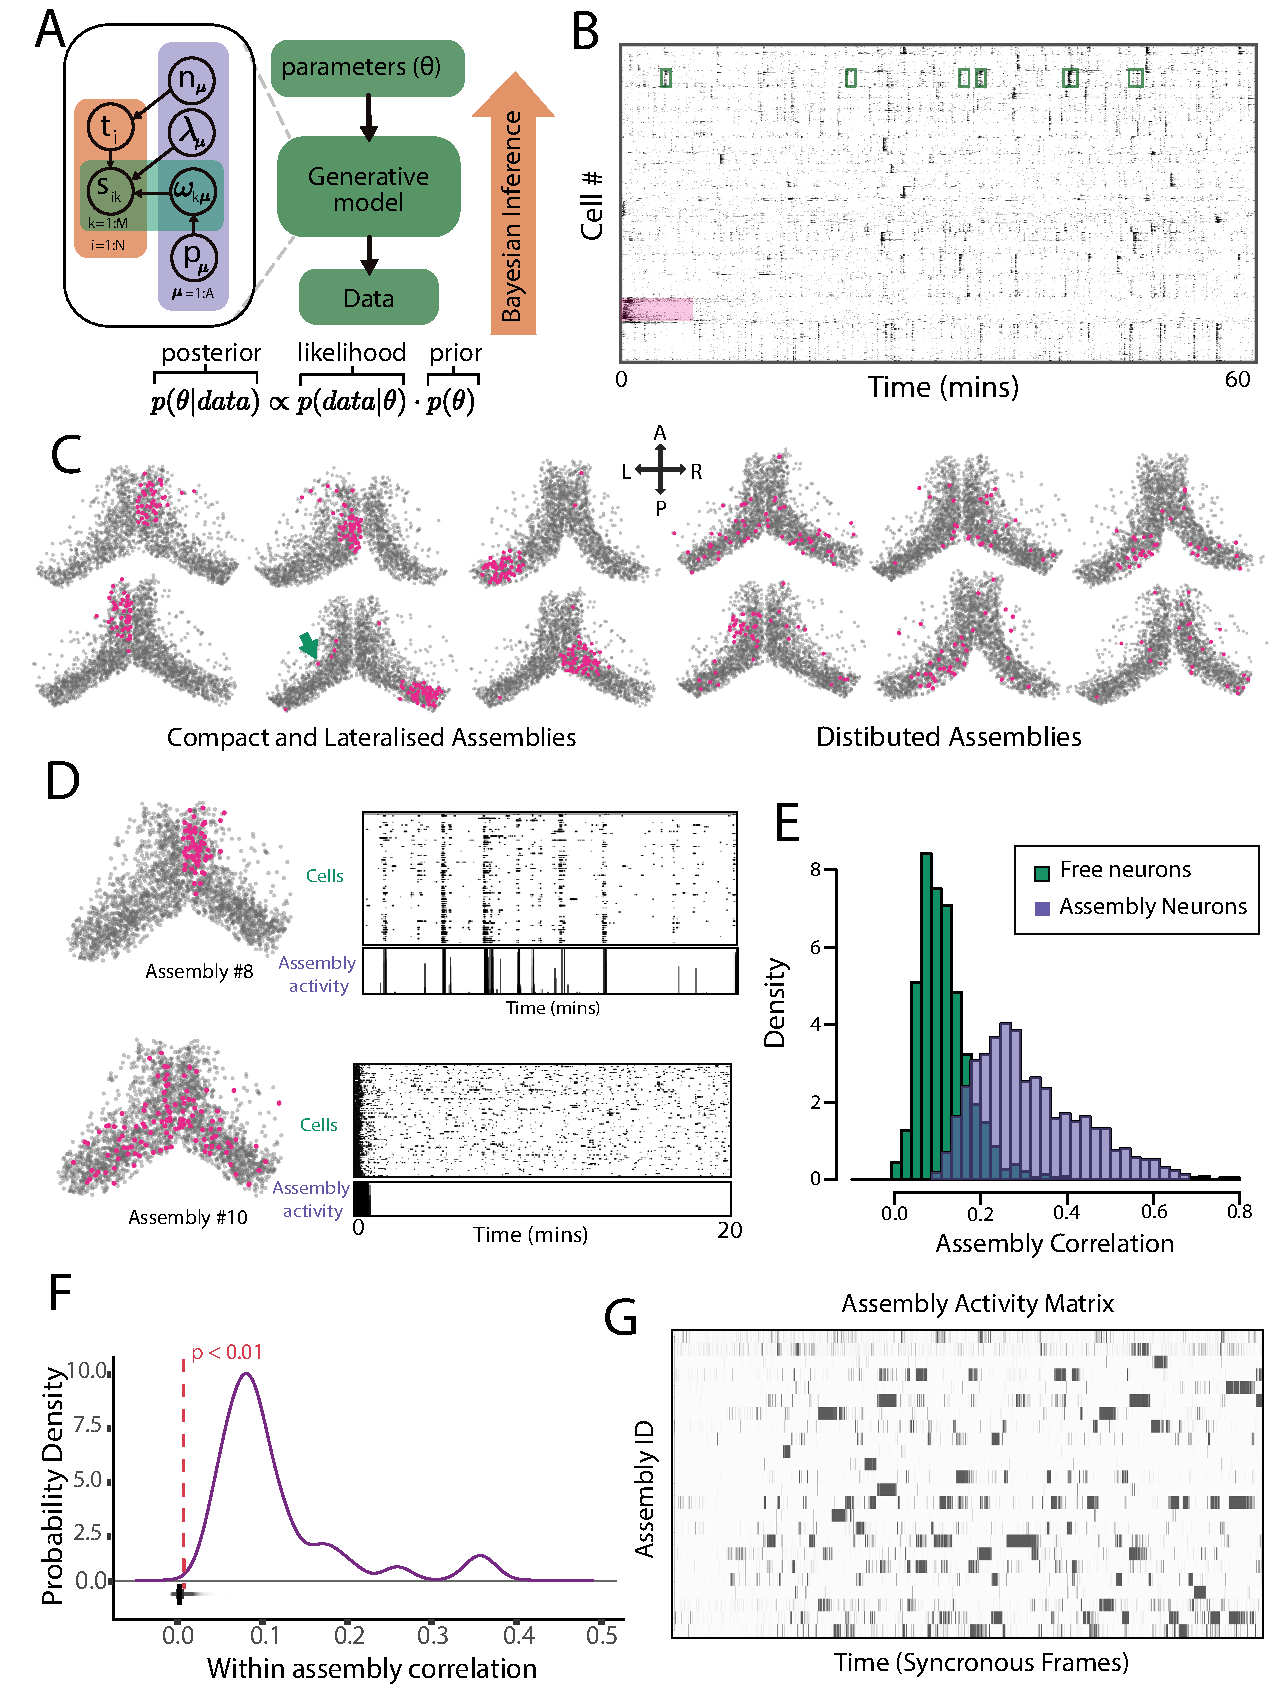
\includegraphics[width =  0.8\paperwidth]{Figures/R1_F4.jpg}}
            \caption[\label{fig:R1_F4} \textbf{Identifying neural assemblies using BINA.}] {\label{fig:R1_F4} \textbf{Identifying neural assemblies using BINA. (A)} A schematic explaining the components of the \gls{bina} method for identifying neural assemblies. The method contains a generative model which describes the assignment of neurons to assemblies and the firing properties of both those neurons and their assemblies. In this model neuronal activity of $N$ neurons is organised into $A$ assemblies over $M$ timeframes. Each neuron $i$ is given a single assembly assignment $t_{i}$ which is drawn from the categorical distribution. Here the probability of belonging to an assembly $\mu$ is given by $n_{\mu}$. \textit{(continued...)}}
            \end{figure}
            \clearpage
            \begin{figure}[!ht]
            \captionsetup{labelformat=adja-page}
            \ContinuedFloat
            \caption[]{Each assembly $\mu$ can occupy a ON/OFF state ($\omega_{k\mu} = \{0,1\}$) at each time $k$ which is drawn from a Bernoulli distribution with the assembly specific probability $P_{\mu}$. The parameters $\lambda\mu(1)$ and $\lambda\mu(0)$ represent the probabilities that neurons belonging an assembly μ fire when their assembly is active or inactive respectively. This generates the activity matrix $S_{ik}$ which represents the activity of each neuron $i$ and each timepoint $k$. To infer the values of these parameters, this matrix $S_{ik}$ is replaced by the actual spontaneous activity dataset (as shown in  \textbf{\ref{fig:R1_F3}A}).  Bayesian inference can then invert this generative process to give the posterior distribution of these parameter values given the spontaneous activity data. For clarity the priors have been excluded from this graphical representation of the generative model \textbf{(B)} A raster plot where neurons that has been sorted by assembly membership. This shows that assembly members fire together synchronously at multiple time points in the recording (an example is highlighted by the green boxes). Some assemblies where found to fire transiently at the beginning of the recording (highlighted in pink). Such assemblies are likely to be responding to the sound of the resonant scanner or the movement of the objective and were therefore excluded. \textbf{(C)} Assembly maps showing the spatial distribution of neural assemblies within the tectum. Some compact and lateralised assemblies had "satellite cells" in the contralateral hemisphere (green arrow). \textbf{(D) Top:} A compact assembly with its corresponding raster plot showing the timepoints that its cells are active. The plot of assembly activity shows time points that the assembly is active as inferred by BINA. \textbf{bottom:} An example of a distributed assembly that responding transiently at the beginning of the  recording. \textbf{(E)} Histograms showing the density of correlations (Pearsons) between either free neurons or assembly neurons with assembly activity. \textbf{F)} Within assembly correlation is significantly greater than randomly generated assemblies of the same size. \textbf{(G)} A raster plot showing the time points that each assembly was active, as inferred by the BINA \label{fig:R1_F4}}
    \end{figure}  
      
\clearpage
\subsection{Identifying neural assemblies in the tectum}
The findings above are consistent with previous findings showing that spontaneous activity in the tectum is organised into assemblies (\cite{Romano2015}; \cite{Avitan2017}; \cite{Pietri2017}). However, relatively little is known about the properties of these assemblies. For example, the number of neurons per assembly, the firing properties of the assemblies themselves, the behaviour of neurons within the assemblies and how assemblies interact with one another are not known. Because all of these features may be relevant for how the tectum encodes information and generates behaviour they are important metrics to quantify. For this purpose I used a Bayesian inference method (\gls{bina}) that has been previously shown to outperform other methods in validation tests. Furthermore, unlike other existing methods, \gls{bina} provides a statistical framework that quantifies the uncertainty of assembly parameters and can also infer the timepoints at which each assembly is active, allowing for the dynamics of the assembly to be quantified. 

Briefly \gls{bina} relies on a generative model to  describe the observed assembly activity through a set of unobserved (latent) features, $Z$, and model parameters, $\theta$. Contained within this model is the idea that there are neurons, these neurons are organised into assemblies and at each time point each assembly can occupy an activity state of ON or OFF. Neurons themselves can fire when their assembly in ON (synchronous firing) or when it is OFF (asynchronous firing) with certain probabilities. Therefore this model could generate data that resembles the population activity within the tectum given the correct model parameters (such as assembly membership, synchronous and asynchronous firing probabilities). The aim of Bayesian statistics is to invert this process and calculate the probability distribution of these parameters and latent variables conditional to the data using Bayes' theorem: 

\begin{align}
    \overset{\mathrm{Posterior}}{\overbrace{P(Z,\theta|\mathrm{data})}} \propto \overset{\mathrm{Data\;Likelihood}}{\overbrace{P(\mathrm{data},Z|\theta)}}\times \overset{\mathrm{Prior}}{\overbrace{P(\theta)}}
    \label{eq:bayes_theorem}
\end{align}

which expresses this probability in terms of the likelihood of observing the data (given the model parameters) and the prior distribution of the parameters which represents our a priori knowledge about the model. Calculating the full posterior distribution would require complete enumeration of all combinations of $\theta$ which is computationally unfeasible. Therefore \gls{bina} instead draws samples from this distribution using a Gibbs sampler allowing the posterior distribution to be approximated within a short period of time. This method therefore allows for the structure and dynamics of neural assemblies to be inferred from population data (for a graphical representation of the model see \textbf{Figure \ref{fig:R1_F4}A}).

 To apply this method to our data I first reduced the number of frames for each dataset by selecting only those frames where there were more than 15 neurons active. This is because it allowed for the sampler to reach convergence quicker whilst discarding frames where there is unlikely to be assembly activity. \gls{bina} initially assigns all neurons to an assigned to a potential cluster, including cells that may not actually belong to an assembly. As a result, there were a number of clusters which clearly were not assemblies. This is because they were not active at all within the duration of the recording, or contained very small numbers of neurons.  Such clusters do not fit the definition of an assembly ie. groups of neurons that fire together synchronously. Therefore only clusters which had an activity level > 0.5\% and a size larger than 5 neurons were used for subsequent analysis. In addition, only those cells that could be reliably assigned to an assembly in 99\% of the samples from the posterior were considered to belong to that assembly and any non-assigned cells were called "free neurons".

To demonstrate the validity of this method in identifying tectal assemblies in  a raster plot of neuronal activity was sorted by assembly membership. This revealed groups of neurons that were firing together at multiple different points within the recording (\textbf{Figure \ref{fig:R1_F4}B}). The spatial location of each assembly's constituent neurons were then superimposed back onto the tectum to show how they were spatially arranged (\textbf{Figure \ref{fig:R1_F4}C}). The majority of the assemblies were spatially compact, highly lateralised and found to tile the anterior posterior axis of the tectum.  Whilst most assemblies were compact there were a few assemblies that appeared to be more distributed, with constituent neurons spanning the complete extent of the tectum. However, many of these distributed assemblies were found only to be firing synchronously at the beginning of the recording suggesting that rather than being spontaneously active these assemblies were transiently responding to sensory input caused by the microscope starting to image. Therefore any assemblies showing these transient effects were excluded from further analysis because they are unlikely to reflect the preferred network states of the tectum (for examples \textbf{see Figure \ref{fig:R1_F4}B} and \textbf{Figure \ref{fig:R1_F4}D  assembly \# 10}).

Something that is inferred by the BINA method is the timepoints that each assembly is active (\textbf{Figure \ref{fig:R1_F4}D and G}). To ensure that assembly neurons were  correlated with their assembly and that the free neurons were not, the time correlation (Pearsons) between each assigned neuron and the activity of the assembly that it belongs to were calculated. Next the maximum correlation between each free neuron with each of the assemblies was taken. By plotting both these distributions together showed that assembly neurons are far more correlated with assembly activity than the free neurons. This suggests that BINA is able to identify only those neurons which are associated with assembly activity and that the free neurons are far less coupled to these populations.

To see if the retained assemblies could be explained by random groupings of cells within the tectum, null assemblies were generated by randomly picking the equivalent number of neurons to the assembly from all possible neurons in the tectum, this was repeated 2000 times. The mean within assembly correlation coefficent was then calculated for each assembly and its null assemblies by taking the average pairwise correlation between all of the assemblies constituent neurons. This showed that 100\% of assemblies exceed not just their own null distributions but also the null distributions for any assembly in the tectum with a p < 0.01 \textbf{(Figure \ref{fig:R1_F4}F)}. This demonstrates that the \gls{bina} clustering method is capable of isolating groups of neurons that fire together synchronously and reveals spatial structure that is not specified by parameters within the generative model. 
 
\subsection{Quantifying the structure and dynamics of tectal assemblies}
From using this Bayesian inference method it is possible to infer the identity of constituent neurons of an assembly and the timepoints where the assembly is active (\textbf{Figure \ref{fig:R1_F5}A-B}). This allows the structure and dynamics of the assemblies in the tectum to be obtained. To first understand how cells in the tectum were partitioned into these assemblies for all imaged fish. The average number of assemblies in each fish was 41$\pm$11 assemblies and ranged from 24 to 64 (\textbf{Figure \ref{fig:R1_F5}C}). Not all of the active neurons could be assigned reliably to an assembly; between 48\% - 70\% of active neurons were assigned with over 99\% probability to an assembly and the rest were considered to be "free neurons" (\textbf{Figure \ref{fig:R1_F5}D}).  For each fish the number of neurons that were recruited by each assembly showed similar broad distributions and had a mean across fish of 31$\pm$0.38 cells (\textbf{Figure \ref{fig:R1_F5}E}). 

By eye, assemblies in the tectum appeared to exhibit a high degree of spatial organisation by being both spatially compact and highly lateralised. To quantify these observations I generated metrics for both the spatial extent of the assembly and its lateralisation. Firstly, to measure the spatial extent of each assembly, an ellipse was fitted to the 2D distribution of its constituent neurons (visualised in \textbf{Figure \ref{fig:R1_F5}A}) This was achieved by calculating the two eigenvalues ($\xi_1$ and $\xi_2$) of the co-variance matrix of the XY neuronal coordinates within each assembly and then extension was quantified as:

\begin{align}
    E=\pi \sqrt{\xi_1\xi_2}
\end{align}

Lateralisation on the other hand was assessed using the following equation:

\begin{align}
    abs(LI) = abs\left(\frac{L - R}{L + R}\right)
\end{align}

where L is the number of cells within the left tectal hemisphere and R is the number of cells on the right. This gives a lateralisation index (LI) where the absolute value quantifies the degree of laterality which ranges from 0 (assembly is bilateral) to 1 (lateralised to a single hemisphere). To understand if assemblies were significantly compact and lateralised the same metrics were computed for 2000 topographic null models for each assembly. These null models were generated by randomly selecting the same number of neurons from all possible neuron locations in the tectum (spatial null models). This showed that for each fish 73\%$\pm$0.12  of assemblies were significantly compact (p<0.01) when compared to their own null model (\textbf{Figure \ref{fig:R1_F5}F}). Interestingly, each fish showed a slight bi-model distribution with a small number of assemblies occupying a larger spatial extent suggesting that there may be two separate types of assemblies within the tectum, those that are spatially compact and those that are more distributed. Likewise a large number of assemblies also showed high LI values with 78\%$\pm$0.01 being significantly lateralised (p<0.05) (\textbf{Figure \ref{fig:R1_F5}G}). Together these metrics demonstrate that these neural assemblies tend to exhibit a high degree of spatial organisation by being both compact and lateralised.

In addition to the structure of the assemblies I also wanted to understand their within-assembly dynamics. This is possible because within the \gls{bina} clustering method the assembly activity state is inferred as a latent variable within the model. This was used to estimate the frequency with which each assembly was active in events per minute (\textbf{Figure \ref{fig:R1_F5}H}) and most assemblies being active with a frequency of around 2.3$\pm$0.38 events/minute. One feature of assemblies is that their constituent cells can be noisy with not every cell firing when the assembly is active and cells also firing when their assembly is inactive (See \textbf{Figure \ref{fig:R1_F5}B}). This behaviour of neurons within each assembly can be quantified using two probability values: 1) synchrony, which is the probability that a neuron fires when its assembly is active and 2) asynchrony, which is the probability that a neuron fires when its assembly is inactive. All fish showed similar shaped distributions for synchrony with a mean value of 0.2$\pm$0.02, whereas asynchronous firing showed a tighter distribution with much smaller values than synchronous firing of 0.007$\pm$0.0008, indicating that assemblies neurons are far more likely to fire with their assembly rather than in isolation(\textbf{Figure \ref{fig:R1_F5}I-J}). Finally, assemblies in all fish showed significantly greater within assembly correlation when compared to assemblies containing random groupings of assembly neurons 99\%$\pm$0.09 (p < 0.01)(\textbf{Figure \ref{fig:R1_F5}K}). 



\begin{figure}[!ht]
        \center{\includegraphics[width =  0.77\paperwidth]{Figures/R1_F5.jpg}}
            \caption[\label{fig:R1_F5} \textbf{Characterising assembly structure and dynamics}]{\label{fig:R1_F5} \textbf{Characterising assembly structure and dynamics} \textbf{(A)} Parameters quantifying the structure of assemblies can be calculated from the spatial maps of assemblies such as spatial extent which is calculated by fitting an ellipse to its 2D distribution. \textbf{(B)} A plot showing the activity of the constituent neurons of the assembly relative to the the time points that the assembly is active (inferred from the model). This illustrates that not every neuron fires with the assembly every time and neurons can also be active when the assembly is inactive. \textbf{(C)} A bar plot showing the number of assemblies in each fish.  \textbf{(D)} A bar plot showing the percentage of neurons that can be assigned to an assembly with 99\% confidence, these assigned neurons were celled assembly neurons. Any neurons that did not meet this requirement, along with any neurons that belonged to excluded assemblies were called free neurons. \textbf{(E)} A density plot showing the distribution of assembly size in terms of the number of neurons. Grey lines represent single fish and purple thick line is the mean distribution across fish. \textbf{(F)} Density plots for the 2D spatial extent of all assemblies for each fish (orange) compared to their spatial null model (green). \textbf{(G)} Density plots of lateral index for all assemblies for each fish compered to their spatial null models. \textbf{(H)} Density plot of assembly firing frequency. \textbf{(I)} Density plot of synchrony, the probability that a neuron fires when its assembly is active. \textbf{(J)} Density plot of asynchrony which is the probability that a neuron fires when its assembly is in active. \textbf{(K)} Density plot of within assembly correlation for each fish compeared null models.}
      \end{figure}


\subsection{The relationship between assembly structure and dynamics}
Based on the observation that neural assemblies can occupy a range of firing properties I next asked whether these dynamic properties of an assembly could be related to its physical structure. For example, one possibility is that the firing rate of an assembly may be related to its size or compactness. To investigate this possibility correlation (Spearmans rank) was computed pairwise for all assembly parameters. This revealed a number of interesting correlations between structural parameters and  functional parameters. For example, negative correlation was seen between assembly size (number of neurons) and both synchrony and asynchrony parameters whereas a small positive correlation was seen between an assembly's lateral index and its firing frequency (\textbf{Figure \ref{fig:R1_F6}A-B}). Plotting these comparisons as scatter plots showed non-linear relationships between parameters of assembly structure and dynamics. Some of these relationships such as the one between assembly firing frequency and lateral index appeared to be very weakly related. Therefore to understand the relationship more fully a bootstrapping procedure was applied to each correlated pair by recomputing the correlation on subsampled data (20\% of the original dataset size) and was repeated for 20000 iterations. This produced empirical distributions for the correlation values. This showed that assembly size had a strong-moderate negative correlations with synchrony (rho = -0.63 $\pm$ 0.06) and asynchrony (rho = -0.47 $\pm$ 0.08) whereas lateral index and assembly firing frequency showed a weaker positive correlation of (rho =0.37 $\pm$ 0.06). This indicates that the physical structure of the assembly is correlated with its firing frequency and the coupling of neurons within the assembly. 


\begin{figure}[!ht]
        \center{\includegraphics[width =  0.8\paperwidth]{Figures/R1_F6.pdf}}
            \caption[\label{fig:R1_F6} \textbf{Correlation between assembly structure and assembly dynamics}]{\label{fig:R1_F6}\textbf{Correlation between assembly structure and assembly dynamics} \textbf{(A)} Correlation matrix between different assembly parameters. Green colours indicate positive correlations and magenta show negative correlations (Spearmans rank).  \textbf{(B) Top:} Some correlations appeared to be very variable. Therefore to ensure the correlations were genuine and not artifacts of the sampled population, empirical distributions for the correlation were generated by a bootstrapping procedure. For this procedure, 20\% of the data was resampled and the correlation was recomputed. Repeating this process for 20,000 iterations produced  distribution over the possible values of the correlation. \textbf{Bottom:} Scatter plots showing the relationship between assembly size (number of neurons) with both synchrony and asynchrony and between lateral index and assembly firing frequency. In all of these scatter plots the points are displayed over their smoothed density in order to visualise the relationship between the two variables.
            }
      \end{figure}

\subsection{Functional properties of assemblies are uniform across the tectum}
Assemblies tile the tectum and cover the full extent of the the anterior posterior axis. However the brain of teleost's is constantly growing throughout the their lifespan with new born neurons constantly being added by neurogenesis (\cite{Boulanger-Weill2019}). In the optic tectum neurogenesis occurs at the caudal-lateral edge in order to add new periventricular neurons to mature tectal circuits (\cite{Schmidt2013NeurogenesisAdult}). Rather than migrating these neurons are pushed away from the caudal-lateral zone by a cellular conveyor belt as new neurons are born (\cite{Boulanger-Weill2017}). This creates a gradient of neural maturity across the anterior posterior axis as neurons are integrated into the tectal circuitry. As a result it may be expected that assemblies may have different properties depending on their location within the tectum based on their maturity. Furthermore, stimulating different regions of the tectum can generate different behavioural output suggesting that assemblies within the tectum may be regionally specialised (\cite{Helmbrecht2018}). To test these ideas the tectal hemispheres across fish were aligned using a rigid body registration and the the center of mass for each assembly was calculated and superimposed onto the tectum (\textbf{Figure \ref{fig:R1_F7}A}).  Only assemblies with a high lateral index (LI > 0.5) were plotted because distributed assemblies are by definition not spatially localise within the tectum. The plotted centers were then coloured by the certain parameter values for that assembly. This showed that there was no spatial bias for structural assembly parameters such as its size (number of neurons) or area (\textbf{Figure \ref{fig:R1_F7}B-C}). Furthermore, assembly dynamics such as firing frequency, synchrony and asynchrony also appeared to be uniform across the spatial extent of the tectum. This suggests that the properties of the assemblies do not show regional specialisation in any of the parameters that were measured (\textbf{Figure \ref{fig:R1_F7}D-F}).

    \begin{figure}[!htb]
        \center{\includegraphics[width = 0.8\paperwidth]{R1_F7.pdf}}
        \caption[\label{fig:R1_F7} \textbf{Assemblies properties are invariant to their location within the tectum.}]{\label{fig:R1_F7} \textbf{Assemblies properties are invariant to their location within the tectum. (A)} Assembly centers (black points) were calculated by computing the center of mass from an assembly's constituent neurons and superimposed onto the tectum. Assembly centers were colored by \textbf{(B)} assembly's size (number of neurons), \textbf{(C)} Spatial extent, \textbf{(D)} Synchrony, \textbf{(E)} asychrony and  \textbf{(F)} assembly firing frequency. None of these parameters indicated regional specialisation in terms of the assemblies.}
      \end{figure}
      
\subsection{Correlated activity between assemblies suggests that they are organised into distinct sub-networks}
One advantage of using BINA compeared to other existing assembly identification methods is that it also infers the time-points where the neural assemblies are active (\textbf{Figure \ref{fig:R1_F8}A}). This provides a lower dimensional representation of tectal activity which can be used to explore the interactions and correlations between different neural assemblies. This gives an opportunity to understand if there is spatial organisation in the temporal correlations between tectal assemblies. For example, do certain assemblies in one region of the tectum always correlate with those in another region.  To do this pairwise correlations (Pearson's) were calculated for each assembly (\textbf{Figure \ref{fig:R1_F8}B}). These were then used to construct a graph (\textbf{Figure \ref{fig:R1_F8}C}). This graph was then clustered to produce subnetworks of assemblies which had a high degree of correlation with each other  (see \textbf{Materials and methods}) (\cite{Newman2004FindingNetworks}; \cite{Csardi2006TheResearch}). These sub-networks mainly consisted on tectal assemblies that were found in the same tectal hemisphere. Coloring the maps of tectal assemblies by their sub-network identity suggested that there was very little correlation between anterior-posterior assemblies (\textbf{Figure \ref{fig:R1_F8}D}). Consistent with this there was decreased correlation  ipsilateral assemblies that were located further away from each other within the tectum and there almost no correlated activity between anterior-posterior assembly pairs (\textbf{Figure \ref{fig:R1_F8}E-F}). These results suggest that there maybe functional segregation between assemblies located in the anterior and posterior locations of the tectum.


  \begin{figure}[!htb]
        \center{\includegraphics[width = 0.8\paperwidth]{Figures/Assembly_interations.pdf}}
        \caption[\label{fig:R1_F8} \textbf{Sub-networks of correlated tectal assemblies}]{\label{fig:R1_F8} \textbf{Sub-networks of correlated tectal assemblies. (A)} A raster plot showing the inferred timepoints that each assembly is active (black). Here assemblies have been ordered according to their sub-network identity shown in C. \textbf{(B)} Correlation matrix showing the pairwise correlation (Pearson's) between the inferred activity trace for each assembly. This matrix has been sorted based on sub-network identity shown in C, revealing high levels of correlation between  assemblies in the same sub-network.\textbf{(C)} A graphical representation of assembly correlations. In this graph each assembly is represented by a node and the length of the edge between nodes is proportional to the correlation, with shorter nodes indicating higher correlations. Node shape indicates which tectal hemisphere the assembly is from. \textbf{(D)} Assembly maps coloured by their subnetwork identity as in C. Note that neighbouring assemblies tend to be clustered together and that correlations between ipsilateral assemblies in anterior and posterior tectum are rarely seen. \textbf{(E)} Scatter plot showing assembly correlation by the physical distance between assembly centers. \textbf{(F)} Percentage of assembly pairs with a correlation greater than a threshold, $\lambda$, as $\lambda$ is increased. Ipsilateral pairs of assemblies positioned at opposite poles of the tectum (anterior-posterior) show very little correlation with each other compeared to anterior-anterior pairs or posterior-posterior pairs.}
      \end{figure}


\clearpage

\section{Discussion}
The aim of this chapter was to describe how population activity is structured in the visual system under normal conditions and at an age where visually guided behaviour is already present. To do this I recorded the spontaneous neural activity that is present in the optic tectum of 7 \gls{dpf} larval zebrafish and quantified features of the population activity. As in previous studies I found that this population activity is spatiotemporally organised into compact neural assemblies that tile the tectum. I characterised the structure and dynamics of these assemblies using the statistical inference method BINA. Interestingly, correlations were found that suggest that the physical organisation of an assembly may be related to its activity. Finally, these assemblies can also be segregated into sub-networks based on their correlation, this showed that there was very little correlation between anterior-posterior assembly pairs. This understanding of how tectal activity is organised provides a way to investigate how the spatial organisation and dynamics of population activity is shaped by the visual environment during development in subsequent chapters.

\subsection{Mapping the network architecture of the tectum through spontaneous activity}
Even in the absence of external input sensory regions of the brain maintain high levels of activity. Historically, this activity was thought to be noise and was seen to interfere with brain computations (\cite{Faisal2008NoiseSystem}; \cite{Tolhurst1983TheCortex}). However the advance of modern recording techniques has changed this view due to the observation that spontaneous activity manifested in the form of highly organised spatial and temporal patterns which showed striking similarities to evoked activity and activity underlying behaviour (\cite{Kenet2003}; \cite{Luczak2007}; \cite{Luczak2009}; \cite{Miller2014}; \cite{Carrillo-Reid2015}; \cite{Romano2015}). Like previous studies in zebrafish I found that spontaneous activity in our data could be grouped into neural assemblies, the majority of which were spatially compact (\cite{Romano2015}; \cite{Avitan2017}). Investigating the relationship between spontaneous and evoked activity \cite{Romano2015} found that constituent neurons of such assemblies are tuned to the same location in visual space and are activated by a light spot with an angular size of 4$^\circ$. This corresponds to the approximate size of paramecia on the retina at point that hunting behaviour is initiated (\cite{Bianco2015}). Furthermore, assembly activations were found to correlate with tail movements that resembled those seen in hunting larvae (\cite{Romano2015}).  As the optic tectum is integral for hunting it is possible that, in periods of minimal sensory drive,  spontaneous activity replays the constraints of circuitry that is required for the recognition and capture of prey (\cite{Romano2015}; \cite{Marachlian2018PrinciplesTectum}). Under this idea neurons with high connectivity with each other would generate preferred network states and activity in the tectum moves towards these states in what is called "attractor-like" dynamics (\cite{Marachlian2018PrinciplesTectum}). Therefore studying spontaneous activity across development could reveal how these preferred network states of tectum change and how their development is affected by visual experience.

While many neurons could be reliably assigned to a single assembly a large proportion of neurons in the tectum could not. These neurons may belong to assemblies where the main cluster of the assembly did not fall within the imaging plane and was therefore not identified.  An alternative suggestion is that these represent neurons do not belong exclusively to a single assembly. Instead they may represent previously reported "promiscuous" neurons in the cortex that are able to associate with different neural assemblies (\cite{Miller2014}) or "soloists" that are decoupled from the population activity all together (\cite{Okun2015}). While \gls{bina} has an underlying assumption that neurons belong to a single assembly it calculates the probability that a neuron belongs to each assembly. This could be used in the future to understand if some neurons belong to multiple assemblies or none at all.

\subsection{The relationship between assembly structure and dynamics}
 Unlike many previous studies, the Bayesian inference method used in this chapter allowed for intrinsic dynamics of assemblies to be measured through parameters such as assembly synchrony, asynchrony and activity. The underlying pattern of connectivity between its constituent neurons, and therefore its structure,  is likely to be important for setting these dynamics. For example, neurons that are in close proximity in physical space may have a greater influence on each other than neurons that are further away. In this chapter a number of correlations were identified between the assembly structure and  intrinsic dynamics. Firstly,  assemblies with a larger number of neurons have reduced synchrony. One possible explanation for this finding is that neurons have a finite number of connections that they can make. Perhaps to accommodate the integration of additional neurons into the circuit they have to break existing connections. This would cause a larger number of weak, indirect connections within the network and a reduced excitatory drive between assembly members. Therefore spontaneous activation of a small number of neurons would less likely to propagate through the entire network leading to reduced synchronous firing. Secondly, we found a weak relationship between between the laterality of an assembly and its activity. This could indicate that neurons in the same tectal hemisphere are more interconnected than they are between tectal hemispheres. Therefore lateral assemblies through stronger excitatory drive require fewer neurons to recruit the assembly. These results suggest that certain physical properties of these circuits may dictate their dynamics.  Knowing these relationships will be crucial for understanding how the dynamics of an assembly are altered as their pattern of connectivity changes over the course of development.
 
\subsection{Segregation of assembly networks within the tectum}
The optic tectum is constantly growing throughout life with new periventricular neurons being added through neurogenesis at the caudal-lateral and dorso-medial edges (\cite{Boulanger-Weill2019}). This could potentially create a gradient of maturity in neurons within the anterior-posterior axis of the tectum (\cite{Boulanger-Weill2017}) and this gradient may be reflected in the properties of assemblies. Alternatively, the tectum also contains a motor map as stimulating neurons along the anterior-posterior tectal axis can generate different behaviours (\cite{Herrero1998TailGoldfish}; \cite{Helmbrecht2018}; \cite{Fajardo2013ControlZebrafish.}). For example, high angle tail bends that resemble C-turn escape maneuvers can be elicited with a higher probability through stimulation of the posterior regions of tectum. Approaches on the other hand show less of a spatial bias but higher angle tail bends are elicited when the stimulation site is more posterior (\cite{Helmbrecht2018}). As a result, it may be expected that assemblies in different regions of the tectum may have different functional roles and therefore different functional properties. To look for a gradient of maturity or regional specialisation assembly properties were plotted by their location within the tectum and revealed no spatial arrangement. However, correlations between assemblies found in the anterior and posterior regions of the tectum were much weaker that those found in either of those regions alone. This suggests that there may be distinct sub-networks of assemblies restricted to either the anterior or posterior regions of the tectum and may reflect the differences in approach vs avoidance maneuvers caused by these regions. 

\subsection{Limitations of using spontaneous activity to map the functional architecture of the tectum}
Whilst spontaneous activity can be used as a tool to study developing tectal population activity there are a number of potential limitations of the method that should be recognised. Firstly, although spontaneous activity is likely to be correlated between neurons that are connected to each other reflecting the tectal circuitry I cannot exclude the possibility that these neurons are driven by activity from another source. It has been shown that this activity is not driven by spontaneous activity in  the retina because removing the eyes does not significantly impact the structure of spontaneous tectal activity (\cite{Romano2015}). However, the optic tectum receives substantial afferent projections from numerous different brain regions and including information from different sensory modalities (\cite{Nevin2010}). While the larvae are in total darkness, they may be exposed the sound of the microscope and somatosensory stimulation.  Therefore activity related to this stimulation, or the internal state of the organism, could also contribute  to this ongoing tectal activity. Secondly,  it is impossible to distinguish between direct and indirect connectivity between assembly neuron due to the slow kinetics of the calcium probe and imaging speed. This limitation could be overcome in the future through technological advancements in high speed voltage imaging (\cite{Abdelfattah2019BrightImaging}).  Finally, a large number of cells in the tectum were found not to fire throughout the whole duration of the recording. This could mean that recording for an hour is not long enough to reveal all of the functional architecture of the tectum. Alternatively, spontaneous activity may not explore the full repertoire of tectal assembly activations and some assemblies may only be evoked by specific behaviours/visual simulations.

Overall, this chapter provides a description of the structure and dynamics of population activity in the optic tectum under normal rearing conditions and at an age where visually guided behaviour is present. This gives an indication as to what features of population may be affected by environmental enrichment during development and introduces the tools needed to study them.  
    
    \chapter{The effect of environmental enrichment on the development of a visually guided behaviour and tectal population activity}
    \section{Introduction}
Visual environments can vary significantly depending on the geographical location. Even within the same location certain visual features such as colours, texture, vegetation, prey and predators can change drastically between generations, altering the statistics of the visual scene. Thus, genetically similar individuals of the same species occupy many different ecological niches, presenting unique challenges for the visual system (\cite{Engeszer2007ZebrafishField}). As a result, developing animals must learn the statistics of these environments in order to ensure that the ontogeny of visual behavior can either cope with, or exploit a given ecological niche (\cite{Wong2015BehavioralEnvironments}; \cite{Harer2019RevertingFish}; \cite{Gilmour2018PlasticityConditions}).

Flexibility in the face of such environmental diversity is thought to be achieved through mechanisms of experience-dependent plasticity, where incoming sensory input plays an instructive role in the structural and functional formation of neural circuits (\cite{Fox2005ReviewSystems}; \cite{Hooks2007CriticalPlasticity.}). Whilst experience-dependent plasticity is widespread across different species it has been extensively studied in the retinotectal system of anamiotes (namely fish and frogs) (\cite{Ruthazer2010LearningFunction}; \cite{Pratt2016AnDevelopment}). This is because, unlike their amniotic counterparts (chicks, reptiles and mammals) that develop in the absence of visual input, the development of anamiotes is extremely rapid and entirely external. As a result they rely on complex stimulation from the visual world to pattern the early visual system rather than spontaneously induced waves driven from the retina (\cite{Pratt2016AnDevelopment}).
This allows for activity in the tectum to be altered through manipulations to the visual scene over a time period when visually guided behaviour is first emerging (\cite{Ruthazer2004InsightsPerspective}). Furthermore, due to the accessibility and experimental tractability of the tectum, the effect of these manipulations of retinotectal neurons can be readily observed.

During early tectal development coarse retinotopic maps are first established by \gls{rgc} axons following molecular gradients (\cite{Higenell2012ExpressionLaevis}; \cite{Liu2004SwitchingDevelopment}; \cite{Kita2015TopographicZebrafish}). This map is then refined to mature levels of precision by visual experience (\cite{Ruthazer2004InsightsPerspective}). This topographic refinement is driven through dynamic rearrangement of axon branches, selectively stabilising branches in tectal regions that show correlated activity with the developing axon while eliminating those that do not (\cite{Ruthazer2003ControlVivo}; \cite{Munz2014RapidStimulation}; \cite{Ruthazer2004InsightsPerspective}). RGCs also have been shown to modulate the growth of their target neuron's dendrites (\cite{Sin2002DendriteGTPases}), receptive field properties (\cite{Tao2005Activity-dependentFields}; \cite{Dong2012AFields}; \cite{Engert2002MovingNeurons}) and shape local recurrent circuitry through intra-tectal connections (\cite{Pratt2008DevelopmentTectum}; \cite{Xu2011VisualSystem}). 

Many activity dependent effects are thought to be driven by mechanisms of Hebbian plasticty through STDP where the relative timing between pre- and postsynaptic spikes can either strengthen synapses through LTP or weaken them through LTD (\cite{Mu2006SpikeSystem}; \cite{Zhang1998ASynapses}; \cite{Richards2010InLaevis}). Such mechanisms are thought to be mediated by the NMDAR, which acts as a molecular detector of correlated activity. Consistent  with this, many experience-dependent effects can be abolished through selective blockade of the \gls{nmda}  (\cite{Ruthazer2003ControlVivo}; \cite{Engert2002MovingNeurons}; \cite{Sin2002DendriteGTPases}; \cite{Kutsarova2017RulesBrain}). However, Hebbian mechanisms are not the only way that experience shapes the developing visual system. For example, enhanced visual input causes homeostatic changes in the intrinsic excitability of tectal neurons, adjusting their gain to improve stimulus detection (\cite{Aizenman2003VisuallyVivo}; \cite{Pratt2007HomeostaticCircuit}). In contrast, the overall number of cells in the tectum, can be decreased by lowering ambient light levels, suggesting that the neurogensis rate is also regulated by sensory input (\cite{Hall2018VisualTectum}). Together these studies suggest that visual experience has wide spread effects on the development of the tectum.

Recently, a number of studies have taken advantage of the small size and optical clarity of the anamiotic optic tectum to assess the impact of visual experience on developing population activity by using calcium imaging techniques. This is an important development because behaviour and sensory representations are likely to be encoded through the coordinated activity of groups of neurons organised into neural assemblies, rather than single neurons (\cite{Yuste2015}). In tadpoles, visually evoked correlated activity in the tectum increases over the course of development, a process that is abolished through dark rearing or \gls{nmda} blockade (\cite{Xu2011VisualSystem}). In zebrafish, looking at the development of spontaneous activity, it was found that neural assembly number, size and correlation initially increased (2.5-5 \gls{dpf}) and then decreased (5-7 \gls{dpf}) (\cite{Avitan2017}). These tectal neural assemblies were still present in the absence of visual stimulation and, despite removal of the eye, remained predictive of tail movements (\cite{Avitan2017}; \cite{Pietri2017}). This suggests that the development of neural assemblies may rely on principally on intrinsic factors (\cite{Pietri2017}). However, dark rearing caused neural assemblies to be fewer in number, less correlated and severely impacted the ability of the fish to hunt prey (\cite{Avitan2017}). These results indicate that while both intrinsic and extrinsic factors are important for shaping tectal population activity, visual input is necessary for the emergence of hunting behaviour.

In the wild, zebrafish have been found to thrive in different environments scattered across southern Asia and these environments display extreme diversity in terms of the visual features they contain (\cite{Engeszer2007ZebrafishField}).  However, the manipulations that are often used to study how experience shapes the brain in the lab such as dark rearing, monocular deprivation and 
sustained presentations of artificial stimuli are devoid from any naturalistic change that zebrafish would usually experience. Even in the absence of such manipulations normal rearing conditions for model organisms within the lab are highly impoverished, possibly perturbing natural visual system development. An alternative strategy is to use \gls{ee}, rearing conditions that are designed to increase cognitive, motor or sensory stimulation in regards to typical laboratory rearing conditions. In mice, housing with natural bedding,  novel objects and exercises wheels has shown to have wide ranging effects on behaviour, cognitive ability, anxiety and visual system development (\cite{Nithianantharajah2006EnrichedSystem, Beaulieu1990EffectProperties,Beaulieu1987EffectCortex, Mainardi2010EnvironmentalCortex,Sale2007EnvironmentalInhibition}). However, all of these studies enrich multiple different sensory modalities. Currently no study has looked exclusively at the effect of visual enrichment on the developing nervous system and particularly its effect on the emergence of visually guided behaviour and population activity.

In this chapter I sought to understand how natural vision impacts behaviour and development of population activity. larval zebrafish were raised either within normal laboratory rearing conditions (on a shelf in the incubator) or within an enriched visual environment. This \gls{EE} consisted of placing gravel under the petri dish contianing the developing larvae. To examine the effect of enrichment on behaviour \gls{nr} and \gls{gr} fish were allowed to hunt prey within either a \gls{gb} or \gls{wb}. This revealed that GR fish consumed more prey exclusively when hunting over the \gls{gb}, indicating that they may have learnt to use features of the environment to increase their hunting performance. Using 2-photon volumetric imaging to capture the activity of thousands of neurons throughout the optic tectum combined with Bayesian inference techniques showed that \gls{ee} has a profound effect on neural assembly development, with assembly size, firing frequency and synchrony all showing divergent developmental trajectories between 5 and 7 \gls{dpf}. These results suggest that \gls{ee} modifies the structure of population activity in the tectum and that this correlates with improved performance of a tectally-mediated hunting behaviour in a complex visual environment.  Finally, to understand which forms of plasticity may be underlying these experience-dependent changes we generated zebrafish carrying null mutations in \textit{grin2aa} and \textit{grin2ab} which code for isoforms of the NR2A subunit of the \gls{nmda} receptor. In these fish that the effects of \gls{ee} were found to be  blocked, suggesting that the subunit composition of the \gls{nmda} is crucial for mediating the effects of \gls{ee} on functional development of the tectum.
 
\section{Results}
Under laboratory conditions embryonic zebrafish usually develop in a petri dish placed on a shelf within an incubator. These rearing conditions bear little resemblance to the zebrafish's natural habitat lacking many natural features of the visual scene (\cite{Engeszer2007ZebrafishField}). In order to understand how changes in the visual environment affect the development of visually guided behaviour and population activity, zebrafish were either raised under typical lab conditions or in a petri dish rested on a bed of gravel (gravel was also piled around the side of the dish) from 1-7 \gls{dpf}. Both conditions were fed rotifers (live prey) daily from the evening of 4 \gls{dpf} onwards (\textbf{Figure \ref{fig:R2_F1}}).  Placing gravel under the dish exclusively enriches the visual environment by providing natural features that are lacking from the NR condition such as color, texture and diverse spatial frequencies. Furthermore unlike previously used \gls{ee}s, this is purely a visual manipulation with the fish being physically separated from the gravel, therefore the gravel does not provide any potential tactile, olfactory or gustatory stimulation.

\begin{figure}[!ht]
        \center{\includegraphics[width =  0.5\paperwidth]{Figures/R2_F1.pdf}}
            \caption[\textbf{\label{fig:R2_F1}Enriching the visual environment.}]{ \textbf{\label{fig:R2_F1} Enriching the visual environment.} To alter the visual environment zebrafish were either raised over a bed of gravel (GR) or under normal laboratory conditions, with the dish placed on a shelf within the incubator (NR). The NR condition lacks many of the features of the natural world with the fish seeing only the white colour of the incubator and the metal grating of the shelf below their dish.  Adding gravel adds a number of natural features that are absent from the NR condition, such as different colours, curved edges, contrast, different spatial frequencies and stronger optic flow as the fish swims. Therefore GR creates an \gls{ee} when compeared to the NR condition.}
      \end{figure}
      



\subsection{Enrichment enhances prey consumption in a complex visual scene}
To understand the effect of the \gls{ee} on the emergence of visually guided behaviour NR and GR were put through a hunting assay. Based on the different rearing conditions it is possible that any effect on behaviour would be specific to that is specific to the environment. To test this NR and GR fish from the same clutch were added to 35 mm petri dishes containing rotifers and then were placed to hunt for 30 mins over either a \gls{wb} or a \gls{gb}. These dishes were imaged for $\sim$30 seconds prior to and after hunting to record the number of rotifers in the dish (\textbf{Figure \ref{fig:R2_F2} A-C}). The number of rotifers then were manually counted to give before and after readings. This allowed for the number of rotifers consumed in each hunting session to be estimated. Prior to counting the rearing condition was blinded to the counter in order to remove bias.

\clearpage
\begin{figure}[]
        \center{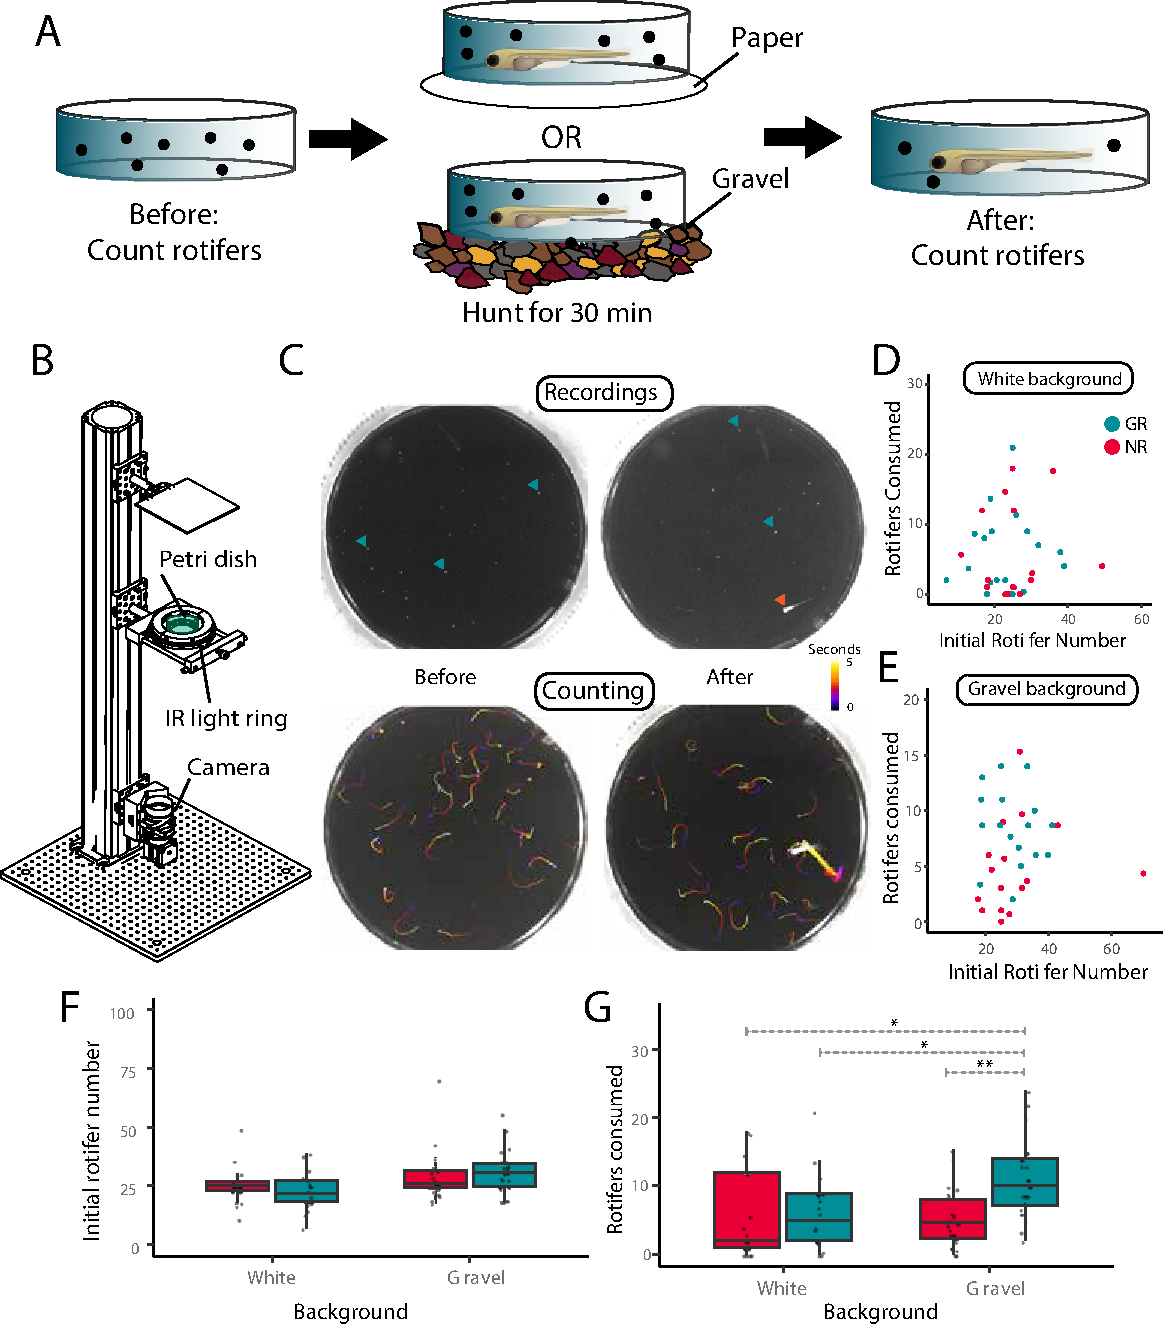
\includegraphics[width =  0.7\paperwidth]{Figures/R2_F2_v3.pdf}}
            \caption[\label{fig:R2_F2} \textbf{The effect of EE on hunting behaviour}]{\label{fig:R2_F2} \textbf{The effect of EE on hunting behaviour} \textbf{(A)} GR and NR fish were subjected to a hunting assay where rotifers were added to a petri dish placed over a white sheet of paper or a bed of gravel. The initial number of rotifers in the dish was counted and fish were then left to hunt for 30 mins. After this period, the number of rotifers was re-counted to estimate the number of rotifers consumed.\textbf{(B)} Behavioural set up for imaging rotifers. The petri dish containing the rotifers was placed in the center of a ring containing infrared LEDs and then imaged by a camera sitting below \textbf{(C) Top:} Example frames from the raw recordings of rotifers before and after hunting (Green arrows point to rotifers; Red arrow points to a zebrafish larvae).\textbf{Bottom:} By colouring frames of the movie by time the swimming trajectories of rotifers could be visualised making them easier to manually count. \textbf{(D-E)} Scatter plots showing the relationship between the initial number of rotifers and the rotifers consumed in 30 mins (\gls{wb}: r = 0.06, p = 0.7, \gls{gb}: r = 0.2, p = 0.09). \textbf{(F)} The initial number of rotifers in the dish prior to hunting was similar across all conditions (WB NR vs WB GR: p = 1, GB NR vs GB GR:  p = 1, WB NR vs GB NR: p = 1, WB GR vs GB GR: p = 0.07,  WB GR vs GB NR:  p = 0.29, WB NR vs GB GR: p = 0.21, Mann Whitney U tests)\textbf{(G)} Box plot showing the number of rotifers consumed within 30 mins when over the white background and gravel background (WB NR vs WB GR: p = 1, GB NR vs GB GR:  p = 0.003, WB NR vs GB NR: p = 1, WB GR vs GB GR: p = 0.026,  WB GR vs GB NR:  p = 1, WB NR vs GB GR: p = 0.26, Mann Whitney U tests). All multiple comparisons were corrected using the Bonfferoni method. \text{*} : p < 0.05; \text{**} : p < 0.01; \text{***}: p < 0.001. box plots represent median and interquartile range.}
      \end{figure}

It may be expected that the density of rotifers could affect the hunting performance of zebrafish. To examine if the number of rotifers affected hunting performance, the initial number of rotifers in the dish was plotted against the number of rotifers consumed for both white and gravel backgrounds.  This showed that there was no relationship between rotifer density and hunting performance (\gls{wb}: r = 0.06, p = 0.7, \gls{gb}: r = 0.2, p = 0.09) (\textbf{Figure \ref{fig:R2_F2} D-E}). Furthermore, the was no significant difference in the initial number of rotfiers for any of the conditions (\textbf{Figure \ref{fig:R2_F2} F}). This indicates that the rotifer density is unlikely to be a confounding factor when looking at the effect of EE on prey consumption. This allowed for the effect of \gls{ee} on prey consumption to be assessed by looking at the total number of rotifers consumed within each of the hunting assays. It revealed that when hunting over the white background GR and NR fish consumed a similar number of rotifers (WB NR vs GR: p = 1) and when hunting over the GB NR fish showed no difference in their food consumption compared to a WB (WB NR vs GB NR: p = 1, WB GR vs GB NR: p = 1). GR fish on the other hand showed a specific increase in the number of prey they were consuming when hunting over the gravel background compeared to all other conditions (GB NR vs GB GR: p = 0.003, WB NR vs GB GR: p =  0.026, WB GR vs GB GR: p =0.026, Mann-Whitney U test, Bonferroni correction)  (\textbf{Figure \ref{fig:R2_F2} G}). These results suggest that EE enhances hunting specifically within the complex visual environment of the \gls{gb}.


\subsection{Spontaneous firing properties of tectal neurons are changed by enrichment}
 In zebrafish, the optic tectum contains the neural circuitry that is responsible for directing prey capture (\cite{Gahtan2005}; \cite{Bianco2015}). As the hunting performance is modified by visual experience it is likely that neural circuitry within the tectum is also changing either as a consequence of changes within the retina, within the tectum itself, or both. Therefore to understand how enrichment alters tectal circuitry spontaneous neural activity was recorded from the optic tectum of NR and GR fish at multiple different stages of development (3, 5, and 7 \gls{dpf}) (\textbf{Figure \ref{fig:R2_F3} A}). This allowed for any changes in population activity between rearing conditions to be identified alongside the developmental timepoint at which they occurred. 
 
 Visual experience has previously been shown to homeostaticly alter the intrinsic excitability of cells (\cite{Aizenman2003VisuallyVivo}; \cite{Pratt2007HomeostaticCircuit}) and modify synaptic plasticity (\cite{Mu2006SpikeSystem}), both of which may affect the activity of single neurons within the tectum. Therefore metrics characterising the activity of single tectal neurons were calculated for fish from both groups at each time point. These results were analysed with a two-way \gls{anova} to look at the effects of rearing condition, age and their interaction. Depending on significance these were followed by post-hoc pairwise comparisons on either the main effects, or in the case of significant interaction, on all pairwise comparisons between the factors (rearing condition and age). All multiple comparisons were corrected using the Benjammani-Hochberg method and only the most salient comparisons are reported here for clarity. This analysis revealed that whilst GR and NR fish had similar numbers of active neuron from 3 - 5 \gls{dpf} there were 20.14\% more active cells in GR fish compared to NR fish at 7 \gls{dpf} (NR vs GR 3 \gls{dpf}: p = 0.14, NR vs GR 5 \gls{dpf}: p = 0.099, NR vs GR 7 \gls{dpf}: p = 0.050, two-way ANOVA, interaction:  F(2,33) =6.82, p = 0.003) (\textbf{Figure \ref{fig:R2_F3} B}).  There was no interaction effect for the firing frequency of tectal neurons but independent main effects were seen for rearing condition (F (1,19) =11.38, p = 0.001) and age (F(2,19) 7.26, p = 0.002) independently with a significant increase in firing frequency over the course of development (3 vs 5 \gls{dpf}: p = 0.001, 3 vs 7 \gls{dpf}: p = 0.004) (\textbf{Figure \ref{fig:R2_F3} C}). Likewise main effects but no interaction were also seen for response amplitude (age:  F(2,19) = 5.094, p = 0.011, rearing condition: F(1,19) = 43.08, p < 0.001) and response duration (rearing condition: F(1,19) = 36.70, p < 0.001) with responses being larger and of longer duration in the GR fish (\textbf{Figure \ref{fig:R2_F3} D-E}).  This indicates that \gls{ee} increases tectal neuron activity by increasing the firing frequency, response amplitude and response duration. However, enrichment has a more delayed effect on the number of active neurons which only showed differences in the later stages of development.

\begin{figure}[]
        \center{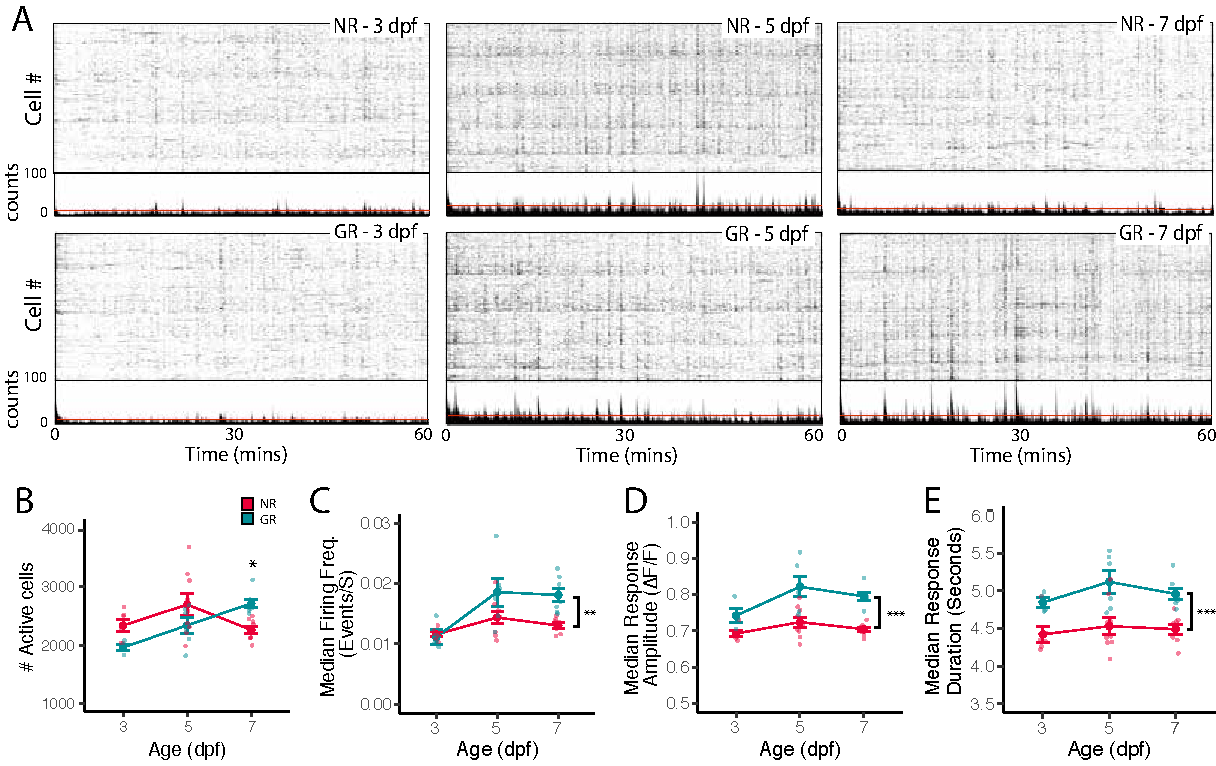
\includegraphics[width =  0.75\paperwidth]{Figures/R2_F3_2.pdf}}
            \caption[\label{fig:R2_F3} \textbf{EE alters the spontaneous properties of single neurons during development.}]{\label{fig:R2_F3} \textbf{EE alters the firing properties of tectal neurons during development. (A)} Representative raster plots of spontaneous activity recorded from the optic tectum of both GR and NR fish at 3, 5, and 7 \gls{dpf}. (NR: 3 \gls{dpf} n = 6, 5 \gls{dpf} n = 9, 7 \gls{dpf} n = 8; GR: 3 \gls{dpf} n = 4, 5 \gls{dpf} = 5, 7 \gls{dpf} = 7). \textbf{(B)} GR fish show an increased number of active cells at 7 \gls{dpf} but not 3 or 5 \gls{dpf} . (GR vs NR: 3 \gls{dpf} p = 0.14, 5 \gls{dpf} p = 0.1, 7 \gls{dpf} p = 0.008; two-way ANOVA, interaction: F(2,33) = 6.82, p =  0.003) \textbf{(C)} Firing frequency was increased in GR fish with respect to NR fish (two-way ANOVA, Age: F(2,19) = 7.6, p = 0.002; Rearing condition: F(1,19) = 11.38, p = 0.002, interaction: f(2,33) =  2.57, p = 0.09). \textbf{(D)} Median response amplitude was increased in GR fish relative to NR fish (two-way ANOVA, Age: F(2,33) = 5.09, p = 0.012; Rearing condition: F(1,33) = 43.07, p < 0.001, interaction: f(2,33) =  1.3, p = 0.29). \textbf{(E)} Median response duration was increased in GR fish compared to NR fish (two-way ANOVA, Age: F(2,33) = 1.69, p = 0.2; Rearing condition: F(1,33) = 36.59, p < 0.001, interaction: f(2,33) =  0.5, p = 0.51). Asterisks highlight contrasts between rearing conditions at each age. All multiple comparisons were corrected using the Benjamani-Hoschberg method. \text{*} : p < 0.05; \text{**} : p < 0.01; \text{***}: p < 0.001. Error bars indicate \gls{sem}.
            }
      \end{figure}



\subsection{Enrichment modifies the developmental trajectory of neural assemblies in the tectum}
Having looked at the effect of \gls{ee} on the development of single neurons properties I next asked whether enrichment alters the structure of population activity in the tectum by analysing the development of tectal assemblies. For this purpose neurons were grouped into assemblies using the BINA clustering method (as described in \textbf{chapter 1}) (\textbf{Figure\ref{fig:R2_F4} A}). 

While the number of assemblies at 5 and 7 dpf was greater than at 3 dpf, rearing conditions had no significant effects on assembly number at any of the three developmental stages (Pooled across rearing condition 3 vs 5 \gls{dpf}: p = 0.023, 3 vs 7 \gls{dpf}: p = 0.030, age: F(2,33) = 4.91, p = 0.01) (\textbf{Figure\ref{fig:R2_F4} B}). The overall percentage of tectal neurons that could be reliably assigned to any of the assemblies  also appeared to increase over development and revealed significant interaction between rearing condition and age (interaction: F (2,33) = 4.45, p = 0.019) with 5 \gls{dpf} GR fish showing a 16\% increase in the number of neurons that could be assigned when compared to NR fish of the same age (5 \gls{dpf} NR vs GR: p = 0.007) (\textbf{Figure\ref{fig:R2_F4} C}). The average number of neurons in each assembly, on the other hand,  followed the same developmental trajectory between GR and NR fish from 3-5 \gls{dpf} but diverged from 5-7 \gls{dpf} resulting in a significant interaction between rearing condition and age (interaction: F(2, 33) =  5.39, p = 0.009) with 7 \gls{dpf} GR fish having 37.4\% more neurons than 7 \gls{dpf} NR fish of the same age (p = 0.0071) (\textbf{Figure\ref{fig:R2_F4} D}). Based on this change it may be expected that the spatial extent of assemblies was also affected. However, there was no interaction between rearing condition and age for the spatial extent of assemblies in the tectum (interaction: F(2, 33) =  0.18, p =  0.85) (\textbf{Figure\ref{fig:R2_F4} E}). In addition, the laterality of the assemblies was also similar between GR and NR fish at all time points, resulting in no interaction (interaction: F(2, 33) =  1.69, p =  0.19). However there was a main effect of age (age: F (2,33) = 5.84, p = 0.007) with assemblies of both rearing conditions combined becoming more lateralised over development (3 vs 5 \gls{dpf}: p = 0.05, 3 vs 7: p = 0.003) (\textbf{Figure\ref{fig:R2_F4} F}). 

 In order to measure the effect of enrichment on assembly dynamics, I plotted assembly frequency, synchrony, and asynchrony against time for each group. Both assembly firing frequency and synchrony in GR fish followed the trajectory of NR fish from 3 - 5 \gls{dpf} but then diverged from 5 - 7 \gls{dpf}. This resulted in the assemblies of 7 \gls{dpf} GR fish being more active (p = 0.044) and less synchronous (p = 0.045) than those of 7 \gls{dpf} NR fish (\textbf{Figure\ref{fig:R2_F4} G-H}). Assembly asynchrony  however remained largely unaffected by rearing condition and age (interaction:  F(2,33) = 2.69, p = 0.083) (\textbf{Figure\ref{fig:R2_F4} I}).

These results demonstrate that the number of assemblies, their spatial extent and laterality are largely unaffected by changing the visual environment with fish from both rearing conditions, showing similar values across development. However, whilst the assemblies of GR and NR fish appear to recruit similar numbers of neurons in early development their developmental trajectories diverge between 5 - 7 \gls{dpf} with the tecta of GR fish possessing much larger assemblies. Furthermore, this divergent change in the developmental trajectory of assemblies is also seen in their dynamics with GR fish showing increased firing frequency and decreased synchrony at 7 \gls{dpf}. These findings suggest that there is a specific developmental time-point, between 5 and 7 \gls{dpf}, during which the visual environment can profoundly alter the developmental trajectory of tectal dynamics.

\begin{figure}[!ht]
        \center{\includegraphics[width =  0.78\paperwidth]{Figures/R2_F4_V2.pdf}}
            \caption[\label{fig:R2_F4} \textbf{The effect of EE on the development on tectal neural assemblies}]{\label{fig:R2_F4} \textbf{The effect of EE on the development on tectal neural assemblies (A)} Raster plots with tectal neurons sorted by their assembly membership for GR and NR fish at 3, 5 and 7 \gls{dpf}. \textbf{(B)} Assembly number increased over the course of development and was unaffected by rearing condition (Age: 3 vs 5 \gls{dpf} p =  0.009, 3 vs 7 \gls{dpf} p = 0.01, 5 vs 7 \gls{dpf} p =  0.64; two way ANOVA, Age: F(2,33) = 4.92, p = 0.013, Rearing condition: F(1,33) = 0.006, p = 0.94, interaction: f(2,33) = 1.81, p = 0.18). \textbf{(C)} The proportion of neural assemblies that can be assigned to an assembly in GR fish is larger at 5 \gls{dpf} than NR fish (GR vs NR: 3 \gls{dpf}  p = 0.28, 5 \gls{dpf} p < 0.001, 7 \gls{dpf} p = 0.28; two way ANOVA, interaction: F(2,33) = 4.45, p = 0.02). \textbf{(D)} The average assembly size, in terms of the number of neurons it recruits, is the same in GR and NR fish at 3 and 5 \gls{dpf} but GR fish have larger assemblies at 7 \gls{dpf} (NR vs GR: 3 \gls{dpf} p = 0.9, 5 \gls{dpf} p = 0.7, 7 \gls{dpf}  p = 0.002; two-way ANOVA, interaction: F(2,33) = 5.4, p = 0.009).  \textbf{(E)} The spatial extent of the assemblies was unaffected by age and rearing condition (two-way ANOVA, Age: F(2,33) = 2.23, p = 0.12, Rearing condition: F(1,33) = 1.39, p = 0.25, interaction: F(2,33) = 0.17, p = 0.85). \textbf{(F)} Assembly laterality was unaffected by rearing condition but increased from 3 \gls{dpf} onwards (3 vs 5 \gls{dpf}: p = 0.04, 3 vs 7 \gls{dpf}: p = 0.003, 5 vs 7 \gls{dpf}: p = 0.81; two way ANOVA, Age: F(2,33) = 5.84, p = 0.007, Rearing condition: F(1,33) = 1.36, p = 0.25, Interaction: F(2,33) = 1.69, p = 0.19). \textbf{(G)} Assembly firing frequency is increased at 7 \gls{dpf} but not at 3 and 5 \gls{dpf} (NR vs GR: 3 \gls{dpf} p = 0.96, 5 \gls{dpf} p = 0.52, 7 \gls{dpf} p =  0.015; two way ANOVA (with white adjustment), interaction = F(2,33) = 3.53, p = 0.04). \textbf{(H)} Assembly synchrony is similar at 3 and 5 \gls{dpf} but is lower in GR fish at 7 \gls{dpf} (NR vs GR: 3 \gls{dpf} p = 0.16, 5 \gls{dpf} p = 0.99, 7 \gls{dpf} p = 0.027, two way ANOVA, Interaction: F(2,33) = 4.67, p = 0.01). \textbf{(I)} Assembly Asynchrony was reduced in GR fish with no effect of age (two way ANOVA, Age: F(2,33) = 1.41, p = 0.26, Rearing condition: F(1,33) = 7.6, p = 0.009, Interaction: f(2,33) = 2.69, p = 0.08). All multiple comparisons were corrected using the Benajamani-Hoschberg method. \text{*} : p < 0.05; \text{**} : p < 0.01; \text{***}: p < 0.001. Error bars indicate SEM.
            }
      \end{figure}

\clearpage

\subsection{The NR2A subunit of the NMDA receptor is required for 
enrichment-dependent development of tectal function.}

The observation that neural assembly development is only affected by EE from 5-7 dpf suggests that there is a switch in development which causes visual experience to start shaping the development of tectal assemblies. Based on this, I next wanted to understand what might be causing this switch  and what types of plasticity might be underlying assembly formation. Hebbian plasticity allows for the modification of synaptic strength between neurons based on the degree of correlated activity and is known to regulate many experience-dependent changes in the brain (\cite{Feldman2012}; \cite{Ruthazer2003ControlVivo}, \cite{Mu2006SpikeSystem}; \cite{Fox2005ReviewSystems}). At the population level, Hebbian plasticity could facilitate the activity dependent formation of neural assemblies by strengthening the connections between neurons that coactively respond to visual features (\cite{Hebb1949}; \cite{Carrillo-Reid2016}). Key to this process is the NMDAR which acts as a coincidence detector between pre- and postsynaptic activity (\cite{Nowak1984MagnesiumNeurones}; \cite{Malenka2004LTPRiches}). In mammals, NMDARs undergo an activity dependent developmental switch, where NR2B containing NMDAR are replaced by those containing the NR2A subunit (\cite{Monyer1994DevelopmentalReceptors}; \cite{Sans2000ASynapses}; \cite{Sheng1994ChangingCortex}; \cite{Liu2004SwitchingDevelopment}). This change in the NMDARs subunit composition alters the channel's kinetics, with NR2A subunits being open for a shorter amount of time, reducing the overall influx of calcium through the channel pore (\cite{Chen1999Subtype-dependenceProbability}, \cite{Erreger2005Subunit-specificProfiles}; \cite{Sobczyk2005NMDASpines}). It is thought that the functional consequence of this change is that NR2A containing synapses are more likely to undergo LTD than NR2B containing synapses (\cite{Yashiro2008RegulationMetaplasticity}). Furthermore, this development switch has been implicated in regulating experience-dependent changes in the visual cortex  (\cite{Fagiolini2003SeparableSignaling}) and its expression is also regulated by visual experience (\cite{Philpot2001VisualCortex}; \cite{Carmignoto1992Activity-dependentCortex}; \cite{Yashiro2005VisualCortex}). This suggests that the NR2A subunit is important for regulating experience-dependent changes in the developing brain by altering synaptic plasticity.  Whilst it is not established whether a switch in NMDAR subunit composition occurs in zebrafish, data from a recent RNAseq database indicates that the expression of NR2A mRNA lags behind that of the NR2B in development (\cite{Petryszak2016ExpressionPlants};\cite{White2017AZebrafish}). Alongside this \textit{in situ} hybridisation images from our group and others have demonstrated that NR2A is expressed in both the retina (\cite{Cox2005MolecularZebrafish}) and the tectum (Issop et al., unpublished). Therefore it is possible that a similar developmental switch may underlie the experience-dependent changes on tectal assembly formation that are seen between 5-7 \gls{dpf}.

\begin{figure}[!ht]
        \center{\includegraphics[width =  0.75\paperwidth]{Figures/R2_F5.pdf}}
            \caption[\label{fig:R2_F5} \textbf{Deletion of \textit{grin2a} genes encoding isoforms of the NR2A receptor.}]{\label{fig:R2_F5} \textbf{Deletion of \textit{Grin2a} genes encoding isoforms of the NR2A receptor.} Regions of DNA at the start of exon 1 were targeted for mutation by TALENs, this resulted in double strand breaks in both \textit{grin2aa} and \textit{grin2ab}. Errors in DNA repair lead to 5 bp insertion (GTTCT) and a 4 bp deletion (TCCA) in the \textit{grin2aa} gene and a 8 bp deletion (ATGGTCTT) in \textit{grin2ab}. Both mutations induced frameshifts in the coding sequence, resulting in premature stop codons which predict truncated proteins (This zebrafish line was generated by Dr Paul hunter) These mutations were then introduced into the \textit{HuC:H2B-GCaMP6s} line through multiple crosses. The sequences in this figure were used in these crosses to identify \textit{grin2aa} and \textit{grin2ab} deletions (See \textbf{Materials and methods}).
            }
      \end{figure}


To investigate if the NR2A subunit plays a role in regulating the effects of EE on assembly formation our lab created a double knock out zebrafish line of both genes encoding the NR2A subunit, known as \textit{grin2aa} and \textit{grin2ab} (created by Dr Paul hunter). This \gls{grin} DKO was originally generated in the \textit{HuC:GCaMP5} line where GCaMP is cytosolic. Therefore, I introduced the \gls{dko} to the \textit{nls-GCaMP6s} background through a series of crosses so that its neural activity could be compeared to \gls{wt} fish which also express \textit{nls-GCaMP6s}  (see \textbf{Materials and methods}). These \textit{grin2a} DKO fish were then NR or GR and at 7 \gls{dpf} spontaneous tectal activity was imaged and compared to \gls{wt} NR and GR fish (\gls{grin2a} NR n = 4, \gls{grin2a} GR n = 4)(\textbf{Figure \ref{fig:R2_F6} A}). 

Firstly, changes in the activity of tectal neurons were examined between these conditions and were analysed using a two-way ANOVA to examine interaction between rearing condition and genotype. Significant interaction was seen between genotype and rearing condition for the number of active cells in the tectum (F (1,33) = 7.21, p = 0.014), their median firing frequency (interaction: F(1,33) = 7.08, p = 0.015), median response amplitude (interaction: F(1,33) = 4.44, p = 0.001) and median response duration (interaction: F(1,33) = 14.44, p < 0.001). This is due to the fact, as I have previously shown, that EE had significant effects on the activity of neurons within the tectum of WT fish with GR WT having $\sim$20\% more active neurons (p = 0.015), a $\sim$38\% increase in firing frequency (p = 0.004) and responses that were around  $\sim$12\%  larger (p < 0.001) and $\sim$10\% longer (p < 0.001) than those of NR \gls{wt} fish.  However, in the \gls{grin} mutant no differences between GR and NR fish were seen in any of these properties (number active cells: p = 0.33 , firing frequency:  p = 0.93, response amplitude: p = 0.45, response duration: p = 0.41) (\textbf{Figure \ref{fig:R2_F6} B-D}). This indicates that the NR2A subunit may be critical for the observed effect of \gls{ee} on the activity of tectal neurons. 

\begin{figure}[!ht]
        \center{\includegraphics[width =  0.8\paperwidth]{Figures/R2_F6_snp_3.pdf}}
            \caption[\label{fig:R2_F6} \textbf{Experience induced changes on the activity of single neurons are abolished in the \textit{grin2a} DKO.}]{\label{fig:R2_F6} \textbf{Experience induced changes on the activity of single neurons are abolished in the \textit{grin2a} DKO. (A)} Raster plots of spontaneous tectal activity in \gls{wt} and \gls{grin} mutants that have been both NR and GR. All recordings were taken at 7 \gls{dpf} (\gls{wt} NR: n = 8, \gls{wt} GR: n = 7, \gls{grin} NR = 3, \gls{grin} GR n = 4) \textbf{(B)} Total number of active cells is unaffected by \gls{ee} in the \textit{grin2a} mutant (\gls{wt} NR vs \gls{grin} NR:  p = 0.38, \gls{wt} NR vs GR: p = 0.009, \gls{grin} NR vs GR: p = 0.33;  two-way ANOVA, Interaction F (1,19) = 7.21, p = 0.014). \textbf{(C)} Firing frequency of \textit{grin2a} NR fish does not increase as a result of gravel rearing (\gls{wt} NR vs \gls{grin} NR:  p = 0.93, \gls{wt} NR vs GR: p = 0.004, \gls{grin} NR vs GR: p = 0.93;  two-way ANOVA, Interaction F (1,19) = 7.08, p = 0.015). \textbf{(D)} NR \textit{grin2a} tectal neuron responses were larger in amplitude than their \gls{wt} counterparts and do not change as a results of enrichment (\gls{wt} NR vs \gls{grin} NR:  p < 0.0001 , \gls{wt} NR vs GR: p = 0.004, \gls{grin} NR vs GR: p = 0.45;  two-way ANOVA, Interaction F (1,19) = 26.0, p = 10$^{-6}$). \textbf{(E)} The duration of tectal responses is unaltered by gravel rearing in the \textit{grin2a} mutant  (\gls{wt} NR vs \gls{grin} NR: p = 0.11 , \gls{wt} NR vs GR: p = 0.0003, \gls{grin} NR vs GR: p = 0.4;  two-way ANOVA, Interaction F (1,19) = 26.0, p = 10$^{-6}$).  All multiple comparisons were corrected using the Benajamani-Hoschberg method. \text{*} : p < 0.05; \text{**} : p < 0.01; \text{***}: p < 0.001. Box plots represent
            median and interquartile range.}
     \end{figure}

To understand if the knockout also perturbed the effect of enrichment on the formation of neural assemblies, neural responses were clustered using BINA and assembly properties were compared between conditions (\textbf{Figure \ref{fig:R2_F7} A}). No significant interaction was seen for assembly number or the percentage of tectal cells that could be assigned to any of the assemblies. However, both were affected by genotype with \textit{grin2a} DKO fish having  $\sim$12 less assemblies on average (Genotype: F(1,19) = 9.59, p = .006) and a lower proportion of neurons in the tectum being assigned to those assemblies (Genotype: F(1,19) =  9.59, p = 0.006) (\textbf{Figure \ref{fig:R2_F7}B-C}). Significant interaction however was present for the average size of each assembly in terms of the number of neurons they contain (interaction: F(1,19) = 4.72, p = 0.04). This was because while EE increased the average number of neurons in tectal assemblies in WT fish (p = 0.001) it had no effect on those in the \gls{grin} DKO (p = 0.53). Instead both NR \gls{grin} DKOs and GR \gls{grin} DKOs had assemblies that were similar in size to those seen in NR \gls{wt}s (NR \gls{wt} vs NR Grin: p = 0.17; NR \gls{wt} vs GR \gls{wt}: p = 0.17), suggesting that the effect of EE was blocked (\textbf{Figure \ref{fig:R2_F7}D}).
 Other parameters quantifying assembly spatial structure such as the assemblies spatial extent and laterality were unaffected by rearing condition or genotype (\textbf{Figure \ref{fig:R2_F7}E-F}. However, similarly to assembly size, assembly firing frequency was affected by an interaction between rearing condition and genotype (interaction: F(1,22) = 11.97, p = 0.0026) and the interaction term for assembly synchrony was very close to approaching significance (interaction: p = 0.06) (\textbf{Figure \ref{fig:R2_F7}G-H}). This is because while gravel rearing led to an increase in firing frequency (p<0.001) and decrease in synchrony in the \gls{wt} fish there was no observable difference between GR Grins and NR Grins in either of these parameters. Finally, no differences were seen in assembly asynchrony between any of the conditions (\textbf{Figure \ref{fig:R2_F7}I}). 

Overall, this demonstrates that although the \textit{grin2a} DKOs may have slightly less neural assemblies than \gls{wt} fish these existing assemblies are comparable to \gls{wt} NR fish in terms of their structure and dynamics indicating a similar level of maturity.  Critically whilst gravel rearing \gls{wt} fish can cause significant changes in assembly size, firing frequency and synchrony GR \textit{grin2a} DKOs show no differences in any these parameters from NR \textit{grin2a} DKOs. Therefore the effect of enrichment on both global properties of the tectum and the formation of local assemblies is blocked in  \textit{grin2a} DKOs and indicates that the NR2A subunit is necessary for these experience-dependent changes to occur.


\clearpage
\begin{figure}[!ht]
        \captionsetup{}
        \centering
        \includegraphics[width =  0.78\paperwidth]{Figures/R2_F7_1.pdf}
       \caption[\label{fig:R2_F7} \textbf{The effect of enrichment on assembly formation is abolished in the \textit{grin2a} DKO fish.}]{\label{fig:R2_F7} \textbf{The effect of enrichment on assembly formation is abolished in the \textit{grin2a} DKO fish. (A)} Raster plots for \gls{wt} and \textit{grin2a} DKOs that have either been NR or GR. In these plots the cell responses have been sorted by their assembly membership as given by the BINA clustering. \textbf{(B)} The number of assemblies was reduced in \textit{grin2a} mutants and enrichment had no effect on assembly number in either condition (two-way ANOVA, Genotype: F(1,19) = 9.59, p = 0.006, Rearing conditions: F(1,19) =  0.77, p = 0.39, Interaction: F(1,19) = 0.21, p = 0.64). \textbf{(C)} The percentage of neurons in the tectum that are assigned to neural assemblies is reduced in the \textit{grin2a} DKOs and there was no effect of enrichment for either condition (two-way ANOVA, Genotype: F(1,19) = 8.56, p = 0.009, Rearing conditions: F(1,19) =  0.51, p = 0.48, Interaction:  F(1,19) = 1.97, p = 0.18). \textbf{(D)} The average number of neurons in an assembly was increased in the \gls{wt} but not in the \textit{grin2a} mutant as a result of gravel rearing (\gls{wt} NR vs \gls{grin} NR: p = 0.18, \gls{wt} NR vs GR: p = 0.001, \gls{grin} NR vs GR: p = 0.53; two-way ANOVA, Interaction: F (1,19) = 4.72, p = 0.043). \textbf{(E)} The spatial extent of neural assemblies in the tectum was unaffected by genotype and rearing condition (two-way ANOVA, Genotype: F(1,19) = 0.003, p = 0.95, Rearing condition: F(1,19) = 0.65, p = 0.43, Interaction: F(1,19) = 0.002, p = 0.97). \textbf{(F)} Assembly laterality was similar across rearing condition and genotype (two-way ANOVA, Genotype: F (1,19) = 0.21, p = 0.64, Rearing Condition:  F(1,19) = 2.54, p = 0.12, Interaction: F(1,19) = 1.68, p = 0.21). \textbf{(G)}  The enrichment effect on assembly activity was not present in the \textit{grin2a} mutant (NR \gls{wt} vs GR: p = 0.68, \gls{wt} NR vs GR: p < 0.001, \gls{grin} NR vs GR: p = 0.63; two-way ANOVA, Interaction: F(1,19) = 11.97, p =  0.002). \textit{(Continued...)}} 
    \end{figure}
    \clearpage
    \begin{figure}[!ht]
    \captionsetup{labelformat=adja-page}
    \ContinuedFloat
    \caption[]{ \textbf{(H)} Assembly synchrony was reduced by gravel rearing in the WT fish (WT GR vs NR: p<0.05) but was unaltered by rearing condition in the \gls{grin} DKO (\gls{grin} GR vs NR: p>0.05)(*the stat for two-way anova is missing due to covid-19 lockdown*). \textbf{(I)} Assembly asynchrony was similar across all rearing conditions and genotypes (two-way ANOVA, Genotype: F(1,19) = 3.21, p = 0.089, Rearing condition: F(1,19) = 1.46, p = 0.24, Interation: F(1,19) = 1.65, p = 0.21)  \text{*} : p < 0.05; \text{**} : p < 0.01; \text{***}: p < 0.001. The p values quoted on these boxplot represent the value of significant ANOVA interaction terms}
    \label{label{fig:R2_F7}}
\end{figure}



\section{Discussion}
 The aim of this chapter was to understand how visual experience shapes the development of visually-guided behaviour and functional properties within the tectum. To investigate this zebrafish larvae were raised in different visual environments where they were either exposed to normal laboratory conditions or \gls{ee} or EE with a gravel background. This simple manipulation of the visual scene resulted in changes in the performance of hunting behaviour with GR fish consuming more paramecia than NR fish  when they hunt over a GB but not when they hunt over a WB. In addition gravel rearing appeared to have two main effects on developing population activity. Firstly, at multiple developmental stages individual tectal neurons showed an increase in firing frequency, response amplitude and response duration in GR fish. Secondly, enrichment appeared to both increase the number of active neuron in the tectum and to reorganise tectal assemblies by altering both their structure and dynamics. Interestingly these differences in active cell number and assembly organisation were only seen in later development, indicating that there maybe a time window were sensory experience begins to shape the underlying circuitry. Finally, these effects were shown to be blocked through the deletion of genes encoding the NR2A subunit of the \gls{nmda}, implicating this subunit as necessary for these experience-dependent changes to occur.
 
 \subsection{Gravel reared fish consume more prey in the gravel background}
 As an innate behaviour it may be expected that the development of hunting follows a genetically defined trajectory that is largely invariant to experience. However, a number of studies across a range of species have indicated a role for experience in shaping innate behaviours such as learning to hunt prey in hatchling snakes (\cite{Mehta2009EarlySnakes}) and the ability to build effective webs in orb web spiders (\cite{Heiling1999TheAraneidae}). In zebrafish, prey capture is severely impaired by dark rearing, suggesting that some degree of visual experience is necessary for efficient hunting to develop (\cite{Avitan2017}). However, sensory deprivation represents an extreme case that fish are unlikely to naturally experience and it is not clear whether more subtle changes in the statistics of the visual scene can also cause changes in behaviour. Altering the statistics of the visual scene during development through gravel rearing revealed that \gls{ee} had an effect on the ability to consume prey. Specifically, GR fish were found to consume similar numbers of prey to NR fish when hunting over the WB. However, unlike the NR fish, GR fish showed an increase in hunting performance when hunting over the GB. This suggests that gravel rearing is not simply accelerating/enhancing general visual system development because this effect is specific to the gravel environment.  Instead, this may indicate that GR fish have learnt to exploit a feature, or combined features, of the GB to its advantage. For example, GR fish may be using the contextual cues of the textured background to better detect or locate prey. In the WB, where these features are absent, GR fish cannot use it to their advantage and consume the same number of prey as NR fish. The NR fish, having no prior experience of the gravel, have not learned to utilise these features and their hunting performance is therefore unaltered by the visual environment.

Hunting in zebrafish larvae is relatively complex, consisting of a series actions that are chained together in a sequence (\cite{McElligott2005PreyControl}; \cite{Budick2000LocomotorCapture}; \cite{Gahtan2005}; \cite{Patterson2013}). A limitation of the behavioural experiments in this chapter is that they do not show how aspects of this hunting sequence are modified to bring about the difference in prey consumption between NR and GR fish. Recently, a study from our group used detailed tracking of the eyes, tail and prey to show that experience of live food alters multiple aspects of this hunting sequence. These changes lead to an increase in hunting performance when compeared to those that have been raised on dry food (\cite{Lagogiannis2019LearningLarvae}). A similar level of description for GR fish and NR fish when they are hunting over the two backgrounds could be informative for understanding why the GR fish are consuming more prey in the GB. For example, GR fish may engage in hunting routines more often when in the GB, suggesting that they are better at detecting prey. Alternatively, GR fish may make more accurate turns towards the prey, increasing hunting efficacy and indicating that they are better able to localise prey against the GB. Finally, it is possible that the difference in prey consumption is because GR fish are more motivated to hunt, resulting in an increased hunt rate. However, as both groups of fish consume the same amount when hunting over the white background this seems unlikely.

\subsection{Experience modifies population activity within the tectum}
Prey capture is generated by neural circuitry within the optic tectum (\cite{Gahtan2005}; \cite{Bianco2015}). By imaging spontaneous population activity in the tectum it was found that \gls{ee} caused a number of changes to the structure and dynamics of population activity within the tectum. Firstly, enrichment increased the activity of tectal neurons. Secondly, enrichment was found to alter the normal developmental trajectory of tectal assemblies making them larger, more active and less synchronous at 7 \gls{dpf} than those in NR fish. Therefore while previous studies have shown that visual experience is important for zebrafish neural assembly development (\cite{Avitan2017}; \cite{Pietri2017}), the experiments in this chapter show that even subtle changes in the statistics of the visual scene are able to induce observable changes in population activity within the visual system. Furthermore, these results suggest that rather than accelerating tectal assembly development, EE sends them on divergent developmental paths. 

\subsection{Enrichment increases the activity of tectal neurons}
When recording spontaneous activity from the tectum the sample rate of the imaging and kinetics of the calcium probe make it difficult to estimate the true spiking activity of neurons. Despite this, the increase in median response amplitude and duration in GR fish is likely to reflect an increase in the frequency and duration of spike trains. Such changes in activity could be brought about either through homeostatic changes in the intrinsic excitability of neurons (the ease with which a neuron fires an action potential) or through a rearrangement of synaptic connections leading to increased excitatory drive, both of which are known to be modified by visual experience (\cite{Aizenman2003VisuallyVivo}; \cite{Pratt2007HomeostaticCircuit}; \cite{Pratt2008DevelopmentTectum}; \cite{Mu2006SpikeSystem}). Recurrent connectivity in the tectum is generated by local tectal-tectal connections (\cite{Pratt2008DevelopmentTectum}) and as a result even small changes in the intrinsic properties of neurons could greatly impact the spatiotemporal pattern of population activity  (\cite{Pratt2016AnDevelopment}). However,  the activity of single neurons in GR fish was increased prior to any of the changes seen in the structure and dynamics of the neural assemblies. This suggests that EE may acutely raise the intrinsic excitability of cells in the tectum and that this effect may be followed by changes in connectivity, altering the structure and dynamics of neural assemblies.

\subsection{Enriched fish have larger tectal assemblies}
One of the effects of EE on neural assemblies is that they are larger in terms of the number of neurons they contain.  It is not clear what is causing this change since the number of assemblies and percentage of tectal cells that are assigned to any of the assemblies is unchanged. However, the number of active cells in the tectum of GR fish was also found to increase at 7 dpf, potentially correlating with this change in assembly size. There are two potential explanations for these observed changes. Firstly, neurons that are usually inactive could be are "turned on" by \gls{ee}. One previous study demonstrated that many cells in the optic tectum of tadpoles remain silent due to insufficient glutamtergic input. It was found that through exposure to natural visual scenes ("planet earth", BBC) these inactive cells could be converted into spiking neurons and that these changes were driven by synaptic plasticity rather than changes in intrinsic excitability (\cite{vanRheede2015Sensory-EvokedMechanism}). Therefore it is possible that exposure to gravel alters connectivity within the tectum, causing neurons that are usually inactive to be recruited to spontaneously active assemblies. Secondly, this increase in the number of active neurons in the tectum could reflect and increase in the overall number of tectal neurons (active and inactive cells). This is because visual experience in known to modulate the tectal cell number by modifying neurogenesis rates (\cite{Hall2018VisualTectum}). Interestingly, artificially increasing neurogenesis in the visual cortex increased the size of neural assemblies and improved the ability of a mouse to distinguish between similar stimuli (\cite{Fang2017OverproductionDiscrimination}). Based on this, increasing the rate of neurogenesis could potentially cause an increase in the total number of cells in the tectum, leading to larger assemblies in GR fish. This change may specifically help GR to discriminate prey against the complex backgrounds. Imaging high resolution volumetric stacks of the tectum in future experiments would allow for the total number of cells in the tectum to be counted. This would reveal whether the overall number of cells in the tectum is changing, potentially accounting for the change in the number of active neurons and assembly size. 


\subsection{The relationship between spontaneously active tectal assemblies and prey capture}
While it is not yet known if the development of neural assemblies in the tectum is related to the development of behaviour, a number of key aspects of assembly development correlate with changes in hunting behaviour: Firstly, assembly size and spatial correlation peak at 5 \gls{dpf} and decrease toward 7 \gls{dpf} correlating with the emergence of hunting behaviour which is first apparent at 5 \gls{dpf} and then improves towards 7 \gls{dpf} (\cite{Avitan2017}; \cite{Avitan2019}). Secondly, dark rearing zebrafish disrupts the number of neural assemblies and decreases local tectal correlations whilst also reducing hunting performance (\cite{Avitan2017}). Thirdly, I find that \gls{ee} modulates assembly size, activity and synchrony between 5 - 7 \gls{dpf} while also improving hunting performance in the gravel background. Together these results may indicate that intrinsic factors initially group neurons into assemblies that are capable of causing the fish to start snatching at prey. After this initial grouping visual experience then modifies this circuitry, potentially refining the behaviour. 

One additional thing to consider is that while sensory systems are under a selective pressure to produce adaptive behaviour they are also subject to constraints driven by costs associated with the amount of energy the system consumes (\cite{Nevin2010}). Raising neural activity comes at considerable metabolic cost due to the increased Na+/K+ ion pump activity that is required to re-establish a resting membrane potential (\cite{Niven2007FlyCoding}). A corollary of this is that any change that increases activity is likely to outweigh theses metabolic costs and be advantageous for the organisms survival. Therefore the effect of enrichment in increasing the activity of tectal neurons and producing larger more active assemblies is likely to be related to an advantageous change in sensory processing, potentially leading to increased hunting performance, negating the associated metabolic cost.  However, how these changes in spontaneous activity actually \textit{cause} changes in prey capture is still a major unknown. Therefore ideally it would be important to understand how visually evoked activity is altered in the tecta of GR fish, when they are viewing stimuli over either textured background or plain background. This would reveal whether the tectal responses are modulated by the context of the background. Such modulation could potentially enhance the perception of the size, direction of motion or location of the prey - all of which could lead to an increased prey consumption in the GB.

\subsection{The NR2A subunit of the NMDA receptor is required for experience to modify tectal activity}

The formation of neural assemblies is thought to occur through the strengthening of synapses between neighbouring neurons that are synchronised in their spike timing (\cite{Hebb1949} ; \cite{Sejnowski1999}; \cite{Carrillo-Reid2016}). At the synaptic level this is facilitated by the \gls{nmda} (\cite{Feldman2012}, \cite{Zhang1998ASynapses}; \cite{Mu2006SpikeSystem}). In this chapter deleting the NR2A subunit of the \gls{nmda} did not severely disrupt tectal activity nor abolish the formation of neural assemblies. This suggests that the NR2A subunit does not play a role in establishing the initial emergence of neural circuitry within the tectum. In contrast to this, deletion of the NR2A subunit was found to completely abolish all of the experience-dependent effects that were induced by EE in the tecta of WT fish. Whilst this result is still preliminary, it suggests that the NR2A subunit may be necessary for visual experience to modify tectal circuitry. 

Based on the fact that visual experience shapes tectal assemblies from 5 - 7 dpf and that this effect is blocked in the \gls{grin} \gls{dko} could indicate that, as seen in mammals, there is a developmental switch in NMDAR subunit composition. This switch   could regulate the experience-dependent effects in the tectum in a similar manner to its effects on the cortex (\cite{Yashiro2008RegulationMetaplasticity}; \cite{Fagiolini2003SeparableSignaling}). To confirm a switch in the subunit composition it would be necessary to accurately quantify the expression of NR2A and NR2B subunits in the tectum across development.  Even if this switch is not present, other studies have shown that the expression of the NR2A subunit itself can be modulated through visual experience (\cite{Philpot2001VisualCortex}; \cite{Carmignoto1992Activity-dependentCortex}).  As a result gravel rearing may be inducing changes in the subunit composition of synaptic \gls{nmda}s, leading to circuit level modifications. In the \gls{grin} mutant, this experience-dependent change would not be able to take place, blocking the effect of visual experience within the tectum.  Therefore it will be important in future experiments to examine the expression profiles of NR2A and NR2B subunits throughout development in both GR and NR conditions. In addition, it would be integral to examine spontaneous activity at multiple developmental timepoints to understand if this effect is specific to the 5-7 dpf window, or if it is disrupting other aspects of tectal development earlier on. 

Finally, the effect of the \gls{grin} DKO on behaviour has not yet been examined. Based on the results in this chapter, it would be predicted that GR \gls{grin} DKOs do not show an increase in prey consumption when hunting over the gravel background relative to NR \gls{grin} DKOs. This would indicate that the mutant does not only block the effect of enrichment on tectal spontaneous activity but it also blocks the effect of enrichment on behaviour. This would provide further evidence of a relationship between the organisation of spontaneous tectal activity and behaviour. 

Overall, this chapter demonstrates that the visual environment induces correlated changes in both naturalistic behaviour and development of population activity within the optic tectum. Importantly these changes can be blocked by manipulating the \gls{nmda} suggesting that the NR2A subunit underlies these experience-dependent modifications. However, whilst enrichment alters the structure and dynamics of spontaneous activity in the tectum it is unclear how these changes are able to actually \textit{cause} the improvement in hunting performance seen in the GR fish in the GB. The next chapter outlines an experiment to examine whether visually evoked activity in the tectum is changed by \gls{ee}. This experiment attempts to understand whether there are changes associated with how the tectum is processing visual stimuli which could account for the changes seen in the hunting behaviour.













      
      


    
   \chapter{Examining visually evoked activity and behaviour in a virtual reality hunting assay}
   \section{Introduction}
The focus of the previous Chapter was to understand how visual experience during development modifies behaviour and developing spontaneous activity within the tectum. To do this, zebrafish larvae were raised either under normal laboratory rearing conditions or in enriched conditions, where a petri dish was placed over a bed of gravel. These changes in the visual environment were found to have two main effects: 

\begin{enumerate}
    \item  GR fish were found to consume more prey than NR fish when hunting over the GB but not a plain WB. Importantly, this was not due to the NR fish eating less food when hunting over the GB as they consume a similar number of prey in either background. This suggests that during development the GR fish have learnt to exploit a feature/features of the GB and this facilitates them in eating more prey. 
    \item Spontaneously active tectal assemblies in GR fish appear to follow a completely different developmental trajectory to NR between 5 - 7 \gls{dpf}. This resulted in the 7 \gls{dpf} GR fish having neural assemblies that were larger, more active and less synchronous than those seen in the tectum of NR fish. 
\end{enumerate}

While these changes in spontaneous activity demonstrate that EE shapes the development of the tectum, it is difficult to relate changes in the structure and dynamics of spontaneous activity to the changes in hunting behaviour.

Hunting in zebrafish consists of multiple different steps, each of which could be modified by enrichment, to alter prey consumption. First, a fish has to detect a potential target from its surroundings and make a decision on whether it is worth pursuing. Then, if hunting is initiated, the fish converges its eyes and orientates itself towards the prey using a characteristic J-turn, where the tip of the tail bends unilaterally towards the stimulus. This is then followed by a series of minor adjustments in heading direction, as the fish tracks the prey, and ends with a final high velocity strike at the prey (\cite{Budick2000LocomotorCapture}; \cite{Gahtan2005}; \cite{Patterson2013}; \cite{McElligott2005PreyControl}). Based on this sequence of events, there are two potential ways that enriched fish may be using the GB to increase their prey consumption: 1) The GB may help enriched fish in initially detecting prey -  this would allow the fish to engage in more hunting routines thus increasing prey consumption. Or 2) the GB helps enriched fish to better locate their prey, leading to more accurate turns in the hunting sequence, increasing hunting efficiency, although both of these possibilities may not be mutually exclusive.

One possible way that these hypotheses could occur is that the gravel background could contextually modulate the population response in the tectum, altering the perception of prey. This is interesting because the contextual modulation of neural responses when viewing visual scenes is already a well known phenomenon (\cite{Spillmann2015BeyondStimuli}). In the simplest case contextual modulation has previously been shown to alter the receptive field properties of single neurons through center-surround modulation. This is where responses to visual stimuli positioned in the center of the receptive field can be either facilitated, or suppressed, by presenting different visual features such as changes in luminance, contrast or more complex spatiotemporal properties to the surrounding visual space (\cite{Krause2014ContextualCortex}; \cite{Sun2002ContextualPigeons}; \cite{Huang2019NeuralCircuit}). Such modulation has been shown to be most pronounced when the surrounding stimuli mimic the statistics of natural visual scenes rather than those that have been phase scrambled (\cite{Guo2005Centre-surroundCortex}). This has lead to the notion that circuitry in the visual system may utilise contextual modulation as a mechanism to segment natural scenes, allowing salient features to be identified, potentially contributing to "pop-out" phenomena. Furthermore, neurons in the visual system of dark reared animals have been found to exhibit reduced center-surround modulation, suggesting that the structure of of natural scenes is required to shape this form of contextual modulation  (\cite{Pecka2014Experience-DependentScenes}). Therefore it is possible that the responses of neurons in the tecta of GR fish are contextually modulated by the presence of the GB, leading to an enhanced ability to detect or localise the prey and that this ability is acquired through their exposure to the gravel during development. 

To investigate this hypothesis it is necessary to image activity in the tectum when GR and NR fish are viewing prey over the textured and non-textured backgrounds. Whilst imaging visually evoked tectal activity is difficult in freely moving fish, a number of studies have shown that hunting behaviours can be elicited in head fixed preparations, by projecting artificial stimuli onto a screen (\cite{Bianco2011}; \cite{Trivedi2013VisuallyCapture}; \cite{Semmelhack2014}; \cite{Bianco2015}; \cite{Jouary2016ALarvae}). In these preparations eye convergence and J-turns can be elicited by small moving dots of 1$^{\circ}$ to 10$^{\circ}$ in size (\cite{Bianco2015}; \cite{Semmelhack2014}). The size of these dots corresponds to the size of prey on the retina when hunting is initiated in freely swimming fish. This allows for both neural activity in the tectum and the behavioural output to be monitored in a virtual reality hunting assay.

One way to study how much information is encoded about a particular stimulus is to decode certain characteristics from visually evoked activity within the brain (\cite{Glaser2017MachineDecoding}); \cite{Quaglio2017}). In virtual hunting assays prey-like stimuli elicit the activation of spatially compact tectal assemblies (\cite{Bianco2015}; \cite{Romano2015}; \cite{Avitan2016}; \cite{Avitan2019}). Each of the constituent neurons by themselves can be unreliable and have a spatial tuning profiles that are broader than the size of the prey (40$^{\circ}$), leading to poor decoding of stimulus location (\cite{Niell2005FunctionalTectum}; \cite{Romano2015}; \cite{Avitan2016}). Instead, the combined statistics from multiple neurons can provide a much more accurate prediction of a object's position in visual space,  suggesting a population code for stimulus location (\cite{Averbeck2006NeuralComputation}; \cite{Avitan2019}). As a result, the position of very closely spaced stimuli, which producing overlapping patterns of activation in the tectum, can be accurately predicted with simple linear decoding methods (\cite{Avitan2016}; \cite{Avitan2019}). Recently, decoding performance has been used to understand how the ability of the tectum to localise prey changes during development (\cite{Avitan2019}). This work revealed that the sensory representation of prey location becomes more refined over the course of development. Furthermore, not only did this refinement correlate with hunting performance across developmental stages but high decoding performance from the tecta of individual fish accurately predicted their hunting performance. This demonstrates that decoding can be used as a biologically relevant tool to study the neural correlates of changes in hunting performance.

In this chapter I outline a virtual reality hunting experiment designed to understand how the sensory representation of prey-like stimuli in the enriched fish is altered. In this experiment fish are presented with artificial prey at different locations in the visual scene which are separated by a few degrees in visual azimuth. These stimuli evoke overlapping activation patterns in tectal neurons. Importantly the larvae view these stimuli over either an untextured background (grey screen) or textured background (a picture of gravel) while both their tectal activity and tail movements are monitored. The aim of this experiment is to understand how the sensory representation of prey location changes when prey is viewed over textured/non-textured backgrounds, by decoding prey location from the tectum. Based on the results from the hunting assay in Chapter 4, the hypothesis is that GR would show an increased decoding performance when viewing  prey over the textured background whereas the NR would not. Finally, monitoring the fish's tail movements allows for the ability of these different stimuli to induce behaviour to be examined.



\section{Results}
\subsection{The virtual reality hunting assay}
To understand how EE is shaping the sensory representation of prey-like stimuli within the tectum we performed a virtual reality hunting assay which was  designed to mimic features of the hunting assay presented in \textbf{Chapter 4}. To do this GR or NR zebrafish larvae expressing \textif{nls-GCaMP6s} were head fixed at 7 \gls{dpf} in agarose in a cylindrical imaging chamber with their right eye facing a semicircular screen that was covered in a diffusive filter (GR: n = 3, NR: n = 1). Agarose was cut away from both the right eye and the tail, allowing for an unobstructed view of the screen and free movement of the tail. The two-photon microscope objective was positioned above the head of the fish allowing for volumetric imaging of tectum (see \textbf{Materials and methods}). This imaging volume was positioned so that the top slice was always 50$\mu$m below the skin covering the dorsal surface of the tectum. Below the fish sat a high speed behavioural camera which recorded the fishes tail movements through the transparent base of the imaging chamber at 450 Hz. This setup allowed for both tectal activity and tail movement to be monitored for 1 hr while visual stimuli were projected onto the screen (\textbf{Figure \ref{fig:R3_F1}A}). 

Visual stimuli were presented in two blocks which differed in their background. In one block the background was a picture of gravel (textured block) and the other it was simply a grey screen (untextured block). Moving black spots (5$^{\circ}$) were presented over these backgrounds at three different locations in visual azimuth and were presented with multiple repeats (see \textbf{Materials and methods}).  These spots are much closer together than the average spatial tuning of tectal neurons and should therefore cause topographically organised but overlapping patterns of activation (\textbf{Figure \ref{fig:R3_F1}B-C}).

\begin{figure}[!ht]
        \captionsetup{}
        \centering
        \includegraphics[width =  0.75\paperwidth]{Figures/R3_F1.jpg}
       \caption[\label{fig:R3_F1} \textbf{Virtual reality hunting assay to study tectal responses to prey-like stimuli over different backgrounds.}]{\label{fig:R3_F1} \textbf{Virtual reality hunting assay to study tectal responses to prey-like stimuli over different backgrounds. (A)} In the virtual reality setup a larval zebrafish is head fixed in agarose with one eye facing a screen. Prey-like stimuli are projected onto this screen while monitoring neural activity and tail movements. \textbf{(B)} The optic tectum receives the majority of its input from the contralateral eye via \gls{rgc}s which terminate in a topographic fashion within the tectal neuropil. \gls{rgc}s responding to the rear visual field (purple), with their cell bodies situated in the nasal retina, project to the anterior tectum. \gls{rgc}s responding to the frontal visual field (light green) have their cell bodies situated in the temporal retina and project to the posterior region of the tectum. This retinotopic mapping is reflected in the pattern of activity in the downstream tectal neurons. \textbf{(C)} The visual stimulation occurred in 2 blocks that differed in the background that was projected: a textured block (picture of gravel) and an untextured block (grey screen). In these blocks prey-like stimuli, 5$^{\circ}$ spots moving within a 5$^{\circ}$ neighbourhood (dotted arrow), were presented at different locations within the visual azimuth (-10$^{\circ}$, 0$^{\circ}$, +10$^{\circ}$). Here the stimulus location is denoted by the same coloring as in B. \textbf{(D)} Functional imaging data was aligned and segmented using suite2p, allowing for a large number of cells to be segmented across the tectum. Dotted arrow shows the major axis of the tectal neuropil which is used to sort cells based on the anterior posterior position within the tectum. \textbf{(E)} The $\Delta$F/F of 4 tectal cells responding to stimulus presentations in the untextured and textured blocks. Stimulus presentations (epochs) are shaded in grey and the stimulus location is indicated by the colored dot below with the same coloring scheme as in B and C.
    }
\end{figure}


\subsection{Tectal responses to prey-like stimuli}
Visually evoked functional imaging recordings were aligned and segmented to obtain a fluorescence trace for each neuron. These traces were normalised by calculating their $\Delta$F/F and any inactive cells were removed using a min-max procedure (see \textbf{Materials and methods})(\textbf{Figure \ref{fig:R3_F1}D-E}). Of these neurons only a fraction were found to respond to prey-like stimuli. Some neurons, likely to be related to ongoing activity or behaviour, may negatively impact decoding performance because their activity is sporadic, creating noise for the decoder (\cite{Kahn2015ANeurons}). In order to assess the impact of these cells on decoding performance we distinguished neurons that were responding to the stimulus from those that were not. This was achieved by calculating a \gls{ncc} value for each neuron, which quantified the correlation between the neuron and the stimulus (see \textbf{Materials and methods}). Significant correlations between the neuron and the stimulus were defined as NCC values that were 3 standard deviations more than that expected average NCC value for a randomly firing neuron with the same firing probability. This distinguished neurons that were responding to the stimulus from neurons that were not.

Prior to decoding the visually evoked responses were first inspected to understand if there were any major differences between either the untextured and textured blocks or as a result of rearing condition. \textbf{Figure \ref{fig:R3_F2}A} demonstrates that 
 the NCC measure reliably separates those neurons that are responding to the stimulus consistently (NCC neurons) from those that are not (non-NCC neurons) by displaying them in a raster plot. Consistent with the broad tectal responses previously reported  (\cite{Niell2005FunctionalTectum}; \cite{Romano2015}) each prey-like stimulus for in both untextured and textured blocks elicited visual responses in spatially compact but overlapping populations of neurons. These population responses could be visualised by calculating the mean response for each neuron across repetitions of the same stimulus to generate maps of activity across the tectum (\textbf{Figure \ref{fig:R3_F2}B}). Despite the overlapping responses, rough topographic organisation could still be observed by arranging these mean responses based on their position within the anterior-posterior axis of the tectum. This was achieved by manually fitting a line to the major axis of the tectal neuropil (\textbf{Figure \ref{fig:R3_F1}C}) cells were sorted based on their projection onto this line. The mean response of these sorted cells could then be visualised for stimuli in both the untextured and textures blocks. Neural responses for both blocks showed rough topographic order between the 3 stimuli. 

In Chapter 4 EE was found to alter the number of spontaneously active cells and their response amplitude in the tecta of 7 dpf zebrafish. To investigate if enrichment was also affecting the number of active cells during visual stimulation both the total number of active cells in the tectum and the number of NCC neurons were plotted for NR and GR fish (\textbf{Figure \ref{fig:R3_F2}D}). For two GR fish the number of active cells and NCC neurons was low ($\sim$ 700 total active neurons, $\sim$ 250 NCC neurons) whereas for one GR fish and the NR fish these values were much higher ($\sim$ 1700 total active neurons, $\sim$ 500 NCC neurons). This suggests that there may be high within group variability and no major observable difference between the GR and NR fish in terms of total active neuron or NCC neurons. Next the mean response amplitude for each stimulus in both textured and untextured blocks was calculated for each fish. This was done for NCC neurons and for the total number of active cells in the tectum (\textbf{Figure \ref{fig:R3_F2}E}). While responses for NCC neurons appeared to be slightly higher for fish viewing stimuli over the textured background the NR and GR fish showed similar levels of activity. Whereas the mean amplitude for all cells in the tectum was similar between textured and untextured backgrounds and rearing conditions (\textbf{Figure \ref{fig:R3_F2}F}). While more data is needed to examine this question in more detail these results suggest that there is no major difference in activity when the tectum is responding to stimuli. However, it should be noted that these values represent the mean response to a stimulus presentation and not the mean amplitudes of individual calcium events as calculated in \texChapter 4.

\begin{figure}[!ht]
        \captionsetup{}
        \centering
        \includegraphics[width =  0.75\paperwidth]{Figures/R3_F2.pdf}
       \caption[\label{fig:R3_F2} \textbf{Tectal responses to prey-like stimuli.}]{\label{fig:R3_F2} \textbf{Tectal responses to prey-like stimuli. (A)} Active tectal cells were sorted into cells that respond to the stimulus consistently (NCC cells) and cells were activity was not stimulus (non-NCC cells). The reason for this is that ongoing tectal activity or activity associated with behaviour may drastically affect decoding performance, making the results difficult to interpret. By plotting both groups of cells in a raster plot revealed that the NCC measure reliably separated out stimulus responsive cells from ongoing tectal activity. \textbf{(B)} Coloring in cells based on their mean response amplitude for a stimulus showed that prey-like stimuli elicited responses from spatially compact populations of neurons. These populations appeared to show a large degree of overlap. \textbf{(C)} Mean responses for each neuron to each stimulus across the two blocks.  Neurons are ordered by their anterior-posterior position within the tectum (top of plots = posterior, bottom = anterior). This shows overlapping activation patterns but also showed rough topographic order between the 3 stimuli. \textbf{(D)} The number responsive neurons (NCC cells) plotted against the total number of active cells in the the tecta of GR (green) and NR fish (red).  \textbf{(E)} The mean response amplitude for NCC cells responding to each of stimulus positions in both untextured and textured blocks. \textbf{(F)} The mean response amplitude for all tectal cells in each fish for each stimulus presentation in both untextured and textured blocks. 
    }
\end{figure}

\subsection{How to decode stimuli for tectal activity?}
Decoding is a useful tool to understand how much information population activity carries about an external stimulus (\cite{Raposo2014ADecision-making}) and has previously been used to understand how this information changes across different brain regions (\cite{vanderMeer2010TripleTask}), experimental conditions (\cite{Glaser2018PopulationCortex}) and disease states (\cite{Weygandt2012FMRIDisorder}). Here we aim to use decoding performance to understand how the ability of the tectum to distinguish between closely positioned stimuli changes as a result of background complexity and rearing condition. To do so a decoder must learn from a given training dataset a function, $f$, that can predict the stimulus identity, $s$, from the visually evoked population response, $r$:

\begin{equation}
    f: r \rightarrow{s}
\end{equation}

where $r = (r_{1}, ..., r_{n})$ is an $n$ dimensional vector where $n$ is the number of cells and $s$  is the different stimulus positions \{-10$^{\circ}$, 0 -10$^{\circ}$, +10$^{\circ}$\}. Therefore decoding performance is likely to be highly influenced by the choice of decoder because this affects how $f$ is determined. Previous attempts to decode the position of a dot like stimulus from tectal activity have suggested that topography based decoders which utilise the retinotopic organisation of the tectum to decode stimulus location perform poorly, due to map imprecision (\cite{Avitan2016}). An alternative strategy is to a linear decoders which do not use information about the neuron's position in the tectum. Instead, these decoders make classifications based on a linear predictor function by combining a set of weights with the feature vector (i.e the population response vector, $r$) (\cite{Avitan2016}; \cite{Avitan2019})

While non-linear decoders, or statistically optimal decoders (such as maximum likelihood decoders), may yield marginal improvements in decoding performance, linear decoders are preferable in this case because: 1) they are more interpretable by indicating a linear separation between classes, 2) have few hyper-parameters that need to be tuned and 3) are simple to implement. Furthermore linear decoders, such as \gls{lda}, have previously been used to investigate how the tectal representation of stimulus location refines across development (\cite{Avitan2019}). In this study decoding performance was found to be predictive of hunting performance, suggesting that changes in linear decoding performance are relevant to understanding the neural basis for changes in behaviour. To ensure that any decoding result was not an artifact of a single decoder and to understand which linear decoder had best performance on my data, I used two different decoders to decode stimulus position from tectal activity: \gls{lda} and \gls{logreg}. The following sections briefly describe the intuition behind these methods (for both decoders the scikit-learn implementation was used -  see \textcolor{blue}{https://scikit-learn.org/} for a detailed description of the methods)


\subsubsection{Linear Discriminant Analysis}
\gls{lda}, like PCA, attempts to find a lower dimensional representation of the data. Unlike PCA, which tries to maximise the variance of the principle components, LDA maximises the distance between between the means $u$ of the classes $c$ to be decoded whilst minimising their within class variance $V$. This process can be simplified by maximising the following equation: 

\begin{equation}
    J(w) = \frac{| u_{c1} - u_{c2}|^{2}}{V_{c1}^{2} + V_{c2}^{2}}
\end{equation}

This gives a lower dimensional projection  of the data  (usually only 1 or 2 dimensions) that maximises the separation between classes making them easier to decode. LDA learns this projection from a training data set and then can apply the learned transformation to new points (test data). LDA then assumes that each of the classes are normally distributed. Using the mean and standard deviation of each class, it calculates the likelihood that the test point came from each of these classes. Therefore if this assumption of being normally distributed is violated the performance of LDA as a decoder can be impacted.

\begin{figure}[!ht]
        \captionsetup{}
        \centering
        \includegraphics[width =  0.75\paperwidth]{Figures/R3_LDA_explaination.pdf}
       \caption[\label{fig:R3_F3} \textbf{Decoding using LDA}]{\label{fig:R3_F3} \textbf{Decoding using LDA. (A)} A schematic illustrating how LDA reduces dimensionally with respect to PCA given the activity of two neurons responding to two stimuli where stimulus identity is shown in red and green colors. The joint firing of the two neurons is overlapping in both the x and y axis. PCA would attempt to find the principal component that would preserve the maximum variance in the data (PC1). Instead LDA finds the projection of the data that maximises the distance between the means of the classes whilst minimising their scatter (known as the linear discriminant LD1). \textbf{(B)} Data in A projected into the 1D axis LD1. Both Gaussian are easier to separate in this projection. New test points can be classified by projecting them into this space and calculating the likely-hood that the point came from either Gaussian. The point is then assigned to the Gaussian that produced the greater likelihood. The decision boundary between the classes marks the point at which the probability of assignment to either Gaussian is 50\%.
    }
\end{figure}

\subsubsection{Logistic Regression}
\gls{logreg} unlike actual regression does not attempt to predict the numeric variable from a set of inputs. Instead, LogReg calculates the probability that a given input belongs to a certain class (only 2 classes are referred to here for simplicity) and finds a linear boundary that separates these classes. It does this by finding a weight vector $w$ that is orthogonal to this linear boundary such that when input $x$ is multiplied by this weight vector the output $z$, depending on its sign, denotes the class $Y$. Where positive values of $z$ indicate that a point lies above the decision boundary ($Y = 1$) and negative values indicate that the point lies below this decision boundary ($Y = 0$):

 \begin{equation}
    z(x) =  w_{1}x_{1} + w_{2}x_{2} + b     \begin{cases} 
      z < 0, & Y = 0\\
      z = 0,  & \text{x sits on the decision boundary}\\
      z < 0,  & Y = 1 \\ 
   \end{cases}
\end{equation}   

where $b$ is the lines intercept. However, to obtain the probability that x belongs to $Y$ this is fed into a logistic (or sigmoid) function $h(z)$:

\begin{equation}
    h(z) = \frac{1}{1 + e^{-z}}
\end{equation}

This function is takes values between 0 and 1 such that $h(z) = 0$ when $z$ goes to $-\infty$, and $h(z) = 1$ when z goes to $\infty$  and $h(z)$ = 0.5 when $z = 0$ (the decision boundary). Therefore $h(z)$ denotes the probability that Y = 1 and expresses the uncertainty of classifying points that are positioned closer to the decision boundary. This function can be fitted to a training data set by the cross entropy cost function: 

\begin{equation}
    J(h(z), Y) =  \frac{1}{n} \sum_{i = 1}^n Cost(h(z)_{i}, Y_{i})
\end{equation}

where:
\begin{equation}
    Cost(h(z), Y) =  -log(h(z)) & \text{,  if Y = 1}
\end{equation}

and:
\begin{equation}
    Cost(h(z), Y) =  -log(1 - h(z)) & \text{,  if Y = 0}
\end{equation}

As these functions are monotonically decreasing smooth functions they can be minimised using gradient descent, optimising the weight vector and maximising the likelihood of correct assignments. After estimating the parameters of the logistic function using training data the decoder can be used to predict the class of test data. Whilst only two dimensions and two classes are discussed here LogReg can be generalised to multidimensional multi-class problems. Unlike LDA, LogReg does not assume that the classes are normally distributed.

\subsubsection{Constructing population response vectors for decoder training and cross validation}
To train each decoder to predict the stimulus from tectal activity, the mean response for each neuron was calculated for each stimulus epoch. This gave a population response vector for each stimulus presentation in a Neuron x Epoch matrix and a corresponding label denoting the stimulus that elicited that response (\textbf{Figure \ref{fig:R3_F3}A}). The population responses and their corresponding labels were separated based on whether they occurred in an untextured or textured block so that decoding performance could be assessed for the blocks separately (\textbf{Figure \ref{fig:R3_F3}B}). To visualise how separable these population responses were, PCA was applied to these matrices. The transformed points were then plotted against the first two principal components and colored by their stimulus label with the point shape indicating the block. This revealed rough clustering of population responses to the 3 stimuli, indicating shared features between population responses that were evoked by the same stimulus (\textbf{Figure \ref{fig:R3_F3}C}). This indicates that there may be a degree of separability between these clusters that in principle could be well decoded by a linear decoder. However there was also some overlap between these clouds of points suggesting that there may be ambiguity in decoding stimulus identity. It is the extent of this overlap that is of interest because it may change with textured block or rearing condition. 

To assess decoding performance the decoders were trained on the majority of the data. However, each time the models were trained a single population response vector and its corresponding stimulus label were withheld for testing the trained models predictions.  The stimulus identity was then predicted using the trained model from this test point. This process was repeated so that every epoch was tested on once in a leave-one-out cross-validation strategy. The overall decoder performance was calculated as the number of correctly decoded stimuli as a percentage of all epochs tested. 

\subsection{Decoder performance in localising stimuli from tectal activity}
In the previous chapter, enriched fish consumed more prey when hunting over the GB whereas there was no change in the prey consumption of NR fish. One potential explanation for this is that the GR fish have learnt to use the contextual cues of the background to better locate the prey. Based on these results, it may be expected that the GR fish would show increased decoding performance when viewing the prey-like stimuli over the textured background whereas the NR fish would not. To test this, LogReg and LDA were used to decode stimuli from the 3 GR fish and 1 NR fish. To also test the effect of cells that were not responding to the stimulus on decoding performance this process was repeated for NCC cells and all cells (ie. NCC cells and non-NCC cells). This is because non-NCC cells are likely to reflect on-going tectal activity or behaviour and may fire sporadically, reducing decoding performance (\cite{Kahn2015ANeurons}). 

LogReg decoding performance was found to be tightly grouped between fish for both untextured and textured blocks when decoding from the NCC cells (\textbf{Figure \ref{fig:R3_F4}D}). For all GR fish decoding performance was higher in the textured block than the untextured block and appeared to be greater than the NR fish overall. Interestingly, the NR fish also showed a relatively large increase in decoding performance when viewing the stimuli over the textured background compared to the untextured background.  LogReg decoding on all cells resulted in variable decoding results and overall decoding performance was much lower than for the NCC neurons. Most fish (2 GR and 1 NR) still showed an increase in decoding performance in the textured block compared to the untextured block but 1 GR fish showed a decrease. Like LogReg, LDA decoding of NCC neurons also showed increases in decoding performance for most fish from untextured to textured blocks (\textbf{Figure \ref{fig:R3_F4}E}).  LDA decoding of all neurons however was highly variable between fish and was greatly reduced in general. Together these results suggest that fish may show an increased decoding performance when viewing stimuli over the textured background although more data is needed for the NR condition. In addition decoding from all cells together negatively impacts decoding performance overall, possibly due to cells that are not locked to the stimulus creating noise for the decoder. Therefore, to decode the stimulus location reliably from tectal activity only NCC neurons should be used.

Finally, to understand which decoder gave the best decoding performance the results for the NCC neurons for LDA and LogReg for the same fish and block were compared directly. This revealed that LogReg had the best decoding performance over all with an average increase of 5.2\% (p < 0.001, paired t-test) (\textbf{Figure \ref{fig:R3_F4}F}). This indicates that LogReg is the more powerful decoder in terms of segregating the population response space in these fish.


\begin{figure}[!ht]
        \captionsetup{}
        \centering
        \includegraphics[width =  0.75\paperwidth]{Figures/Decoding_figure.pdf}
       \caption[\label{fig:R3_F4} \textbf{Decoding performance in classifying the position of the stimulus from tectal activity}]{\label{fig:R3_F4} \textbf{Decoding performance in classifying the position of the stimulus from tectal activity (A)}  To train the decoders the mean response for each neuron was calculated for each epoch. This gave a matrix of the dimensions (Neuron x Epoch) where each column represented a population response vector. For each population response vector there was corresponding label indicating the stimulus that caused it. \textbf{(B)} Population responses across stimulus repeats sorted by the stimulus that caused them for both the untextured and texutred blocks. \textbf{(C)} A PCA plot visualising population response vectors to each of the visual stimuli. Each point represents a single population response vector reduced to 2 dimensions (i.e the first two principle components - PC1, PC2). All population response vectors displayed are from a single fish. Colors indicate stimulus label and the shape of points denotes the block. \textbf{(D)} Decoding performance using \gls{logreg} to decode stimulus position during the two blocks for both NCC cells and all active cells. \textbf{(E)}  Decoding performance using LDA to decode stimulus position during the two blocks for both NCC cells and all active cells. \textbf{(F)} Comparing the performance of LDA and \gls{logreg} in decoding stimulus location from the same datasets (Untextured and textured blocks for NCC neurons in D). \gls{logreg} showed better decoding performance than LDA in all but one cases. *** = p < 0.001 .
    }
\end{figure}


\subsection{Population responses are more similar between stimulus locations in the textured block}
There are two possible reasons for the increased decoding performance when viewing stimuli over the textured background: 1) the similarity between population responses during stimulus repeats is decreasing when the fish are viewing stimuli over the untextured background, or 2) the population responses between stimuli at different locations are becoming more similar in the untextured block. A similarity index between a pair of vectors is defined by their normalized inner product, representing the cosine of the angle between two vectors:


\begin{equation}
    \cos(\theta) =  \frac{A\cdot B}{\|A\|\|B\|} = \frac{\sum_{i} A_{i} B_{i}}{\sqrt{\sum_{i}A_{i}^{2}} \sqrt{\sum_{i}B_{i}^{2}}}
\end{equation}


where $A$ and $B$ are vectors. If two population response vectors point to in the same direction in n dimensional space then they have a similarity index of 1. This would indicate that the exact same group of neurons are firing whereas a similarity index of 0 would indicate that the vector is orthogonal, with the two population vectors sharing no common neurons (\textbf{Figure \ref{fig:R3_F5}A}). Calculating the pairwise cosine similarity between all population response vectors and sorting them by the stimulus that caused them gives a matrix that makes it easy to visualise the similarity between stimulus repeats (close to the diagonal) and between different stimuli (off diagonal) (\textbf{Figure \ref{fig:R3_F5}B}). Doing this for the textured block reveals a discrete representation where there is high similarity within stimulus repeats but lower similarity between stimuli locations, particularly with those stimuli that are more distant in visual azimuth. For the untextured block this representation appears to far less discrete with increased off diagonal similarity between stimuli locations. To further visualise these differences in similarity between the two stimulus blocks sections of the matrix (denoted by white dotted lines in \textbf{Figure \ref{fig:R3_F5}B}) were averaged. This gave two 3 x 3 matrices where the diagonal represented the mean similarity between stimuli in the same location and the off diagonal values represented the mean similarity between different stimulus locations (\textbf{Figure \ref{fig:R3_F5}C}). Subtracting the averaged cosine similarity matrix for the untextured block from that of the textured block gave a difference in similarly matrix ($\Delta$ cosine similarity), allowing for changes in similarity to be visualised (\textbf{Figure \ref{fig:R3_F5}D}). All fish showed an increase in off diagonal similarity in the untextured block, particularly for stimuli that are further away. This result is consistent with the idea that the textured background may be contextually modifying tectal population activity, allowing for a more discrete representation of stimulus location. This could potentially explain the increased decoding performance for fish when viewing stimuli over the textured block.

\begin{figure}[!ht]
        \captionsetup{}
        \centering
        \includegraphics[width =  0.75\paperwidth]{Figures/R3_F3.pdf}
       \caption[\label{fig:R3_F5} \textbf{Decreased similarity between population responses for different stimuli in the textured block.}]{\label{fig:R3_F5} \textbf{Decreased similarity between population responses for different stimuli in the textured block. (A)} Population response vectors point to a location is response space. If two response vectors point to a similar point in space that means that they are similar in the responses that they contain. This degree of similarity can therefore be calculated by the cosine of the angle between the vectors given by the equation in A. As such a cosine similarity of 1 indicates that the vectors are pointing to the same point in space whereas 0 indicates that they are orthogonal \textbf{(B)} Cosine similarity matrices between population response vectors for the textured and untextured blocks. These have been sorted so that repeats of the same stimulus are neighbouring. This means makes is easy to visualise within stimulus location similarity (close to the diagonal) and between stimulus location similarity (off diagonal). This reveals that when viewing stimuli over the textured background there appears to be decreased similarity between population response compeared to the untextured block. \textbf{(C)} Averaging together the the regions outlined by the dotted lines in B gives a mean summary value for both with stimulus and between stimuli similarities. \textbf{(D)} Taking the difference between the mean similarity matrices gives the difference in cosine similarity ($\Delta$ Cosine similarity). This shows that there is increased similarity between stimulus further away from each other in visual azimuth.  
    }
\end{figure}



\subsection{Tracking and analysing tail movements}
In addition to being able to monitor neural activity, the virtual reality hunting setup also allows for the tail movement of the fish to be monitored using a high speed camera positioned below the imaging chamber. This allows difference in the ability of the prey-like stimuli to induce tail movements as a result of the textured blocks or rearing conditions to be examined. Changes in this ability may indicate a difference in the larvae's detection or perception of prey. The tail movements for only 1 GR fish have been recorded during visual stimulation. However, the following section outlines the pipeline I have developed to analyse this behavioural data.

Accurate quantification of tail motion requires regions of the tail to be tracked. This was achieved by training a \gls{cnn} to recognise equally spaced points along the tail length.  The CNN was implemented using \gls{dlc} (\cite{Mathis2018DeepLabCut:Learning}) (see \textbf{Materials and methods}). To train \gls{dlc} 250 frames from 3 separate tail recordings of spontaneous tail movement were manually labeled. 200 of these frames were used to train the model and 50 were used as a test dataset to evaluate the model performance. This showed that the mean error between predicted labels and manual labels was around 8 pixels. As the width of the tail is around 13 pixels this error was deemed to be acceptable for accurate tracking of tail position. Furthermore, visual inspection of the videos with the predicted markers overlayed revealed that the model tracked the extent of tail well (\textbf{Figure \ref{fig:R3_F6}A}). However, on some high velocity tail movements the tail tip was incorrectly assigned to regions of high luminance in the background caused by infrared light reflections from the microscope objective. This is likely to be due to the poor contrast between the tail tip and background.

To compute a behavioural trace the tail was skeletonized by treating the regions between the markers as separate vectors (bones). The angle of each of these bones relative to the midline was calculated and summed to give the total tail angle. This measure of tail angle is centered at zero when the tail is in line with the body axis and negative deflections indicate tail movements toward the stimulus (\textbf{Figure \ref{fig:R3_F6}B-D)}.  As previously reported head fixed fish were found to move in brief swim bouts with longer inter-bout intervals (\cite{Semmelhack2014}). These bouts could be automatically detected by taking the absolute value of the first derivative of the tail angle trace. Smoothing this trace with a Guassian kernel had the effect of dilating neighbouring tail beats and joining them together. This could then be threshold to each segmented swim bout  (\textbf{Figure \ref{fig:R3_F6}E}) (see \textbf{Materials and methods} for details).

For the one imaged GR fish the likelihood of the tail moving within an epoch was low with only 7.7\% of epochs containing a movement. Whilst this is insufficient data to compare between conditions there are a number of metrics that could be extracted from these within epoch movements including: 1) the probability that the stimulus elicits a tail movement, 2) the latency between stimulus onset and tail movement, 3) the tail angle of the first turn 4) whether this turn was towards the stimulus (\textbf{Figure \ref{fig:R3_F6}F}). Interestingly for the single imaged fish the first turn for all within epoch movements were in the direction of the stimulus, potentially indicating approach behaviours. 

\begin{figure}[!ht]
        \captionsetup{}
        \centering
        \includegraphics[width =  0.7\paperwidth]{Figures/R3_F4.pdf}
       \caption[\label{fig:R3_F6} \textbf{Tracking and analysis of tail movements in head fished larvae.}]{\label{fig:R3_F6} \textbf{Tracking and analysis of tail movements in head fished larvae. (A)} Tail movements were imaged using a high speed camera recording at 450Hz. The tail could then be tracked using a CNN (implemented in DLC) trained on 200 frames extracted from tail recordings of different fish. These images show the tracking of the tail during a single swim bout. Dots show the position of the labelled markers which have been joined with a skeleton of lines between the markers. Markers in these images also show the "trails" of the markers in the previous 3 frames. \textbf{(B)} Schematic showing the position of the eight markers along the tail and the bones of the skeleton in between. \textbf{(C)} A maximum projection of the skeletonized fish tail in a single bout of movement. The tail angle was calculated as the sum of the angles of each bone of the skeleton deviating from the midline. \textbf{(D)}  This gave a behavioural trace representing the tail angle. Here is an example of that trace during one bout of tail movement. \textbf{(E)} Tail movement bouts were detected by calculating the first derivative of the tail angle (purple) and smoothing it with a Gaussian kernel (tail movement trace in red). This had the effect of dilating neighbouring tail beats and joins them together so that they can be segmented using a threshold (green). This allows for each bout to be automatically detected (shaded grey areas). \textbf{(F)} Metrics for bouts occurring within a stimulus epoch can then be estimated. These metrics will include 1) the probability of tail movement, 2) the latency of movement relative to stimulus onset, 3) Tail angle of the first tail movement and 4) whether the movement was towards the stimulus or not. These metrics will allow for the ability of the prey-like stimuli to induce prey-like stimuli to be examined.
       }
\end{figure}

\section{Discussion}
In the previous chapter GR fish were found to consume more prey specifically when hunting over the GB, suggesting a context specific change in their ability to hunt prey. To investigate this hypothesis a virtual reality hunting assay was developed which allowed for simultaneous recording of tectal activity and tail movements while prey-like stimuli were presented at different positions in visual azimuth. Importantly, these stimuli were presented over either an untextured or textured background mimicking the differences in the visual environment in the freely swimming hunting assay.  To understand if the sensory representation of prey location was contextually modulated by the background the position of the stimulus was decoded from visually evoked tectal activity using different decoding methods. This showed that position of the prey-like stimulus could be most accurately decoded from tectal activity using \gls{logreg} and that all fish showed an improvement in decoding performance when viewing the stimulus over the textured background. This preliminary data suggests that population responses in the tectum may be contextually modulated by the textured background to give a more accurate encoding of stimulus position. Finally, tail movements can also be monitored and tracked allowing for accurate quantification of stimulus induced swimming bouts. Therefore this experimental assay could be used in future work to understand how tectal activity and behaviour are modulated by the context of the background.

\subsection{Decoding stimulus location from tectal activity}
Decoding performance is likely to be affected by the choice of decoder and may lead to poor results, or conclusions from changes in decoding performance, if an inadequate decoder is used. Therefore the decoder must be able to decode the stimulus accurately and any changes in decoding performance should also be predictive of changes in behaviour.  As the tectum exhibits a topographic map of visual space it may be expected that stimulus position could be accurately decoded from the position of responding neurons within the tectum. However, while the the tectal topographic map is linear and smooth at the macroscale at the local level it is very imprecise containing a significant number of misplaced cells (\cite{Niell2005FunctionalTectum}; \cite{Romano2017}). This imprecision leads to very poor decoding performance when using topographic decoders (\cite{Avitan2016}). In contrast, statistically optimal decoders such as a maximum likelihood decoders have been found to decode stimulus location from tectal activity with very high performance. Maximum likelihood decoders estimate the statistically most likely stimulus to cause a population response. This is calculated using the full distribution over each neurons response to each stimulus repeat. Whilst a biologically plausible implementation of maximum likelihood decoders has been suggested (\cite{Jazayeri2006OptimalPopulations}) similar decoding performance can also be achieved through linear decoders such as LDA (\cite{Avitan2016}; \cite{Avitan2019}). However, linear decoders are far simpler in their implementation than maximum likelihood decoders and may be closer to the types of computations that are actually performed in the nervous system (\cite{Salinas1994VectorRates}). In addition, linear decoders have recently been used to examine how the tectal representation of stimulus position refines over development (\cite{Avitan2019}). This showed that decoding performance in the regions of the tectum dedicated to the stimuli in the frontal visual field improved correlating with improved prey detection within this region as hunting develops. Furthermore, by performing decoding alongside hunting assays in the same fish showed that decoding performance was predictive of hunting performance at the level of individual fish. While it is not clear how the tectum actually decodes stimulus location, these results show that changes in linear decoding performance are relevant to changes in hunting performance. 

In this chapter I used two linear decoders to predict stimulus position from tectal activity. The reason for doing this was firstly to ensure that changes in decoding performance were not an artifact of using a specific decoder and secondly because the previously used LDA decoder assumes that the data is normally distributed. As a result any changes in decoding performance may be related to violations of this assumption rather than a difference in the tectums ability to localise a stimulus. Therefore in addition to LDA a LogReg decoder was also used as it does not make this assumption. While these decoders were broadly in agreement LogReg had increased decoding performance compeared to LDA in nearly all cases, suggesting that LogReg is better at separating the population response space. This increased performance may reflect that the underlying distribution of population responses are not normally distributed.

Another factor that is likely to affect affect decoding performance is what cells are used for the decoding. For example, while some neurons had a firing patterns that were locked to the stimulus, a larger proportion of tectal neurons did not appear to show visually evoked activity. These neurons, which fire sporadically, are likely to reflect ongoing activity and activity related to behaviour. This sporadic activity, particularly when the training dataset size is small, could negatively impact decoding performance by creating noise (\cite{Kahn2015ANeurons}). To assess the impact of these cells on the ability to decode stimulus location an NCC measure was calculated for each cell and compeared to its own randomly firing null model. This allowed neurons that were responding to the stimulus (NCC cells) to be distinguished from those that were firing more randomly relative to the stimulus (non-NCC cells). Decoding either all tectal cells (NCC and non-NCC cells) or from the NCC cells alone revealed that decoding performance was impacted by ongoing activity in the non-NCC cells. This also increased the variability in decoding performance between fish. Therefore decoding in future experiments should be performed on the NCC neurons alone, as these are the neurons that carry information that is relevant for the task.

\subsection{Contextual modulation of the tectal representation of stimulus location.}

The results from the behavioural assay in Chapter 4 suggest that enriched fish may be learning to use the background to either better detect or locate the prey, leading to higher prey consumption when hunting over the GB. If this is the case it is predicted that decoding performance should be higher when enriched fish view prey over the textured background. By decoding the stimulus location from visually responsive neurons revealed an increase in decoding performance for the GR reared fish when viewing prey-like stimuli over the textured background. This suggests that the tectum is may be encoding more information about the location of each stimulus specifically in the textured block. Furthermore, population responses evoked by stimuli in different locations were found to be less similar when the fish viewed the stimuli over the textured background, leading to a more discrete representation of stimulus location and potentially accounting for the change in decoding performance. Together these results suggest that the representation of the stimuli may be modulated by the context of the background and may allow the fish to better locate prey against textured background.

While these experiments show that there is a clear difference in the population response responses between untextured and textured blocks it is not yet clear what specific features of population activity may be altered to bring about these differences in decoding performance.  However, it is well known that the tuning properties of neurons are not fixed. Instead they can be modulated by features in the visual scene presented outside of the neurons receptive field in multiple species and at different stages of the the visual system (\cite{Krause2014ContextualCortex,Allman1985StimulusNeurons}). This demonstrates that response to a stimulus can be dependent on the context within which the stimulus is presented.  For example, in the optic tectum of pigeons and retina of mice the response of certain direction selective neurons can be influenced by the direction global motion outside of the receptive field location. This suggests that these neurons may be able to distinguish between self motion and local object motion (\cite{Sun2002ContextualPigeons, Sun2006ONRetina}).  Alternatively, other tuning properties such as size and contrast can also be influenced by context (\cite{Krause2014ContextualCortex, Ziemba2018ContextualV2}). Furthermore, identifying salient stimuli such as a vertical bar in a sea of horizontal bars is thought to rely on a mechanism "isofeature" suppression (\cite{Zhaoping2016FromNeuroscience}). Within this mechanism neurons responding to the same/similar features (such as the horizontal bars) tend to suppress each other whereas neurons responding to the different feature (the vertical bar) escape this suppression and fire with higher amplitude.  This leads to a winner take all computation where attention is diverted to the location of the stimulus eliciting the greatest response in both the visual cortex of primates (\cite{Zhaoping2012PropertiesBehavior}; \cite{Allman1985StimulusNeurons}) and the optic tectum of archerfish (\cite{Ben-Tov2015Pop-outFish}).  Such mechanisms of contextual modulation may be important for processing natural visual scenes where salient features such as prey are seldom found in isolation.  Instead natural visual scenes are cluttered with an array of different visual features that need to be perceptually segmented from the salient feature (\cite{Zhaoping2016FromNeuroscience}). Therefore contextual modulation of receptive fields may be important for for identifying prey against the textured background. 

In these current experiments there are a number of features that could be modulated by the presence of the background leading to changes in decoding performance. Firstly, it is possible that the spatial tuning of neurons responding to prey-like stimuli may be sharpened by the context of the textured background. This could lead to decreased similarity between populations responses for the different stimuli in the textured block. To investigate this future experiments could include a larger number of stimulus locations. This would allow for a Gaussian to be fitted to the average response to each stimulus position for a neuron to give a tuning curve. Doing this separately for the textured and untextured block would reveal if the tuning of tectal neurons is changing contextually with the change in background. Alternatively, it could be that the relative motion of the stimulus against the textured background maximally stimulates tectal neurons or that a suppression mechanism from features responding to similar stimuli restricts the spatial spread of responses. Both of which could lead to decreased similarity between population responses in the textured block. These hypotheses could be investigated in future studies either by changing stimulus parameters or by closer inspection of how tectal responses are changing between the two blocks.

 It is possible that contextual modulation of tectal responses is something that is learnt through experience, if this is true then the NR fish should not show increased decoding performance when viewing the stimuli over the textured block. Despite the GR fish showing increased decoding performance overall, the one NR fish that was imaged also showed a increase in decoding performance when viewing stimuli over the textured background. As this is only one fish more data is needed to understand if this decoding performance is also dependent on rearing condition. However, if this result is consistent it would be unclear how this change in decoding performance between the two blocks relates to the increased prey consumption of enriched fish when hunting over the GB and may indicate. This highlights the difficulty of being able to relate changes in the brain to behaviour. Ideally future experiments would use the the same animal for the freely swimming hunting assay and virtual hunting experiments in order to relate changes in the the tectum to hunting performance (\cite{Avitan2019}). Either the overall decoding performance, or the changes in decoding performance between the two blocks, could be correlated with changes in prey consumption at the level of individual fish. This would allow which features may be relevant to the behaviour to be identified.
 
\subsection{Monitoring tail movements within the virtual reality setup}
Head fixed zebrafish larvae are known to respond to prey-like stimuli with movements that are characteristic of hunting (\cite{Bianco2011}; \cite{Bianco2015}; \cite{Semmelhack2014}). These include small unilateral bends of the tail tip towards the stimulus location known as J-turns which, in freely swimming fish, orientate the fish towards the prey. Monitoring these tail movements could potentially allow for the differences in the ability of prey-like stimuli in driving behaviour to be examined when these fish view them over the textured and untextured backgrounds. Such differences would indicate a difference in the ability of these fish to detect or perceive the prey within the context of the background that could potentially lead to increased prey consumption in the freely swimming hunting assay. Therefore tail movements were then tracked using \gls{dlc} giving accurate quantification of the tail kinematics at multiple points along the tail. As in previous studies the one imaged fish in this chapter appeared to move in discrete bouts followed by long inter-bout intervals making them easy to segment (\cite{Semmelhack2014}).  The probability of the fish moving within an epoch was found to be low at around 7 \%. However, this is actually comparable to some other studies with even the most optimal stimuli in one study eliciting hunting behaviours in  5-10 \% of stimulus presentations (\cite{Bianco2015}). It was difficult to see if these movements resembled the J-turns that are known to orientate the fish toward the prey. This may reflect the fact that previous studies have used spots that move across the whole visual field rather than a spot moving within a local neighbourhood and therefore the degree to which the animal needs to turn may be different (\cite{Bianco2011}; \cite{Bianco2015}, \cite{Semmelhack2014}; \cite{Jouary2016ALarvae}). Despite this, all within epoch tail movements in the GR fish were found to elicit tail movements towards the side that the stimulus was being presented. This suggests that they may represent the intent of the fish to approach the stimulus. 

One way to understand if these within epoch movements are related to the initiation of hunting is to also free the eyes of the fish and track their movement (\cite{Bianco2015}). This is because eye convergence only occurs at the initiation of hunting as opposed more ambiguous tail movements which may be related to either hunting, spontaneous swims or struggles in the agarose (\cite{Bianco2015}; \cite{Semmelhack2014}). During decoding experiments the eye position needs to be fixed so that the same region of the retina can be reliably stimulated. However, eye convergence could be used to identify coincident tail movements that may related to hunting in preparations where the eyes are free. Paramaterising these tail bouts using metrics such tail angle, tail beat frequency and bout duration could be used to train a classifier that could distinguish between spontaneous swims and hunting turns. This classifier could then be used to identify J-turns that occur when the eyes are fixed for decoding experiments, similar classifiers have previously been used for the automatic identification of prey capture swims (\cite{Semmelhack2014}). With more data for both GR and NR fish it would be interesting to understand if tail movements differ between the rearing conditions such as the probability that a stimulus causes a prey capture swim or if the latency of the swim changes relative to the stimulus on set. These may indicate a difference in the ability of these fish to detect or perceive the prey-like stimuli, potentially allowing GR fish to engage in hunting episodes with a higher frequency relative to NR fish. 

In summary, this chapter outlines an experimental protocol that could be used to understand how the tectum responds differently to prey-like stimuli when they are presented over different backgrounds. This can be viewed alongside the ability of these stimuli to cause tail movements. Preliminary results suggest that all fish show increased decoding performance when viewing the stimuli over the textured background, suggesting that tectal responses may be contextually modulated. Collecting more data in future experiments may reveal differences between GR and NR fish in how they respond to these prey-like stimuli. This may explain the differences in prey consumption that were observed in chapter 4.




   
   \chapter{Conclusions and perspectives}
   \section{Summary}
In this thesis I investigated the role of visual experience in the development of population activity and visually guided behaviour using zebrafish as a model organism. In particular the effect of EE on hunting performance and developing spontaneous activity were examined. The main findings and developments of this thesis were:
\begin{enumerate}
    \item GR fish consume more prey than NR fish when hunting within the gravel environment but hunt the same amount as NR fish when hunting within the WB.  This environment specific effect suggests that hunting in GR fish is positively modulated by the context of the GB (\textbf{Chapter 4}).
    
    \item Spontaneous activity in the tecta of GR fish relative to NR fish was found to be altered in two ways: a) Single neurons in GR fish were found to have higher response amplitude, duration and firing frequency across multiple stages of development when compared to NR fish. b) Whilst size, firing frequency and synchrony of tectal assemblies were found to be similar between the two rearing conditions in the early stages of development (3-5 dpf), they followed a divergent development trajectory in the later stages (5-7 dpf). As a result, tectal assemblies at 7 dpf were larger, more active and less synchronous in the GR fish.  This shows that the development of the tectal activity is altered by EE (\textbf{Chapter 4}).
    
    \item All experience-dependent changes in the tectum are blocked in a zebrafish line that is a null for both genes encoding the NR2A subunit of the NMDAR. This indicates that the NR2A subunit receptor is necessary for EE to shape tectal population activity, and therefore that Hebbian forms of plasticity may mediate the effects of EE on functional development of the tectum (\textbf{Chapter 4}).
    
    \item A virtual reality hunting assay was developed to understand how the sensory representation of prey-like stimuli changed when these stimuli are viewed over textured/non-textured backgrounds. This was achieved by decoding the stimulus location from tectal activity. Preliminary results show that decoding performance is better when viewing stimuli over a textured background, suggesting that the tectal population response may be modulated by the visual context in which prey-like stimuli are presented (\textbf{Chapter 5}).
\end{enumerate}


Overall, this shows that EE shapes both visually guided behaviour and developing tectal activity in a process that may be dependent on the subunit composition of the NMDA receptor. In addition, it provides an experimental protocol that could be used to relate the effects of EE on behaviour to changes in the tectum in the future.


\section{The importance of natural visual features during development.}
Many approaches studying experience-dependent plasticity in the visual system have attempted to use manipulations that either restrict or reduce the visual information that an organism experiences, relative to normal lab rearing conditions. EE takes the opposite approach by enhancing the sensory experience. In this study placing gravel under the petri dish of developing embryos creates a purely visual EE which uses some natural features that would be present in a natural zebrafish habitat (\cite{Engeszer2007ZebrafishField}). Surprisingly, this subtle manipulation had profound effects on both hunting performance and developing population activity. 

One finding highlighted by the results of this thesis is that the normal laboratory rearing conditions for organisms are likely to be highly impoverished in terms of visual experience. This is something that has been well appreciated in rodent research for a number of years and as a result many labs have incorporated some form of enrichment into their standard rearing protocol (\cite{Bayne2018EnvironmentalPerspectives}). However, zebrafish embryos are still typically placed on a shelf in an incubator which is devoid of any natural features.  
As GR fish were able to consume more prey relative to NR fish it suggests that the normal rearing conditions may be detrimental to visual system development. This has important implications for those studying visual/behavioural neuroscience in zebrafish. This is because studying NR fish may underestimate the types of computation or behavior that the zebrafish visual system is capable of generating in the wild. Furthermore, it is possible that subtle changes in visual rearing conditions, between labs, could produce variability in behaviour and the development of visual system properties. 

The enrichment protocol presented in this thesis was designed to mimic certain features of the natural world by bringing them into the lab. However, it is obvious that this manipulation falls short of delivering the rich visual experience that zebrafish would experience in the wild. Therefore, it is possible that other naturalistic features, such as vegetation or other fish, may also impact visual system development. In addition to this, it is not yet clear from these experiments what features of the gravel are important for shaping the developing brain. For example, is it the colour, the differences in contrast or the different spatial frequencies that are important for its effects on the developing visual system? Or could it be a combination of them all? Future experiments could attempt to isolate which features of the gavel are important for driving the plastic changes observed in this thesis. For example, instead of using actual gravel, a printed picture of gravel could be used instead. This would enable certain features of the background to be manipulated, such as filtering out certain spatial frequencies, colors or changing the contrast in the image. Zebrafish larvae could then be raised over this modified gravel environment so that their neural activity could be imaged and their hunting assessed. If removing a particular visual feature alone is able to block the plastic changes that are usually associated with exposure to gravel this could indicate that that feature is being used to shape the developing visual system and behaviour. Alternatively, it may be that removing any one of  multiple visual features can block the plastic changes in the larvaes behaviour and tectal activity, suggesting that many different features in combination may be critical for inducing the plastic changes seen in this thesis. Furthermore, a major claim of this thesis is that it may be the structure of natural scenes specifically that are important for shaping the behaviour and the developing visual system of zebrafish larvae. Therefore it would be interesting to understand whether it is specifically the structure of natural scenes, or any textured background, that can induce the plastic changes seen in this thesis. To do this, zebrafish larvae could be exposed to a modified version of the gravel where the alignment between different lines in the image has been shifted, creating a phase scrambled version of the gravel background which lacks the spatial structure contained in the original image (\cite{Guo2005Centre-surroundCortex, Pecka2014Experience-DependentScenes}).  

\section{Visually guided behaviour is shaped by the visual environment.}
EE enrichment was found to have a major, yet unexpected, effect on the number of prey that could be consumed by GR fish. This is because GR fish were found to consume more prey that normally reared fish exclusively when they were hunting over the GB. This shows that EE isn't simply accelerating/enhancing visual system development. Instead it suggests that the fish may be using either a specific visual feature, or the combination of many features contained within the background, to their advantage. In the wild, where prey would typically be viewed against a complex background, this could provide a behavioural advantage that promotes survival. Since this thesis has only looked at the number of prey consumed it is not yet clear what aspect of hunting is being altered to facilitate this change. However, the presence of gravel during development may modify the visual system to either enhance the ability of fish to detect or locate prey. It is also possible, yet unlikely, that the presence of of the GB is able to exclusively increase the motivational state of GR fish, resulting in more prey being consumed.

To understand which specific aspect of the behaviour is modified, future experiments could aim to provide a more complete description of the differences in hunting sequences by tracking the tracking GR and NR fish while they are hunting in the two visual environments. In zebrafish, hunting sequences begin with eye convergence and the eyes remain converged for the duration of the hunting sequence (\cite{Bianco2011}). Whilst eye convergence can occur in the absence of prey, these events are extremely rare and almost never exceed a convergence angle of 60$^{\circ}$. Therefore, sustained eye convergence exceeding 60$^{\circ}$ can be used as a measure of hunting event frequency or rate (\cite{Lagogiannis2019LearningLarvae}). An increase in hunt rate in GR fish could be indicative of either a increase in motivational state or in the ability to detect prey. However, if these hunt events in GR fish are initiated when the fish is further away from the prey, it could suggest that the change in hunt frequency is driven by changes in perception rather than motivation. In addition to hunt rate, the heading direction of the fish during hunt sequences relative to the prey could also be examined (\cite{Avitan2019}). This could be used to calculate how accurate the turns in the hunting sequence are. More accurate turns may indicate that the fish is better at locating the prey in visual space, leading to more efficient hunt sequences through on-target turns. Alongside this it may also be expected that the duration of time from the beginning of the hunt sequence to the capture may also be reduced, allowing the fish to hunt more prey within a certain time frame. It may be interesting to do these experiments in petri dishes where both background are contained within the same petri dish ie. one half has a WB and the other has GB. This would allow for the differences in behaviour to be visualised within the same fish as it swims over the two different backgrounds. Any observed changes are likely to reflect differences in the perception of the prey against the background rather that the modulation of motivational state which tend to occur over longer timescales.

Any behavioural changes associated with a change in detection or localisation of the prey could be caused by a contextual modulation of tectal responses which sharpens the perception of prey size, location, contrast and/or direction of motion.  This is plausible as similar modulation of neural responses have been seen in various species (\cite{Krause2014ContextualCortex, Sun2002ContextualPigeons, Sun2006ONRetina, Ziemba2018ContextualV2, Pecka2014Experience-DependentScenes}). One way to test if this is occurring is to allow the zebrafish larvae to hunt artificial prey that are projected onto the side of the petri dish and to image both the heading direction and the eyes. By using artificial prey, it would be possible to modify attributes of the prey such as the contrast, speed and size of the prey when it is presented over both gravel and non-gravel backgrounds. Any difference between GR and NR fish in these behavioural parameters would provide  evidence that the perception of the prey is contextually modulated by the presence of the gravel background rather than the motivation of the fish. However, it would also reveal specifically what attributes in perceiving the prey are being altered to cause the behavioural change.

While the focus of this thesis has been to look at the effect of EE on prey capture, what has not been addressed here is the potential effect on other visually guided behaviours. This may be important because within these early stages of development, in parallel to prey capture, zebrafish are developing a rich repertoire of visually guided behaviours such as the OKR, OMR and predator avoidance (\cite{Naumann2016FromResponse, Portugues2014, Dunn2016}). It is possible that the performance of these behaviours may also be altered by EE and would indicate that the visual environment can play diverse roles on many aspects of developing visuomotor behaviour. 

\section{What does spontaneous activity represent?}
A major component of this work involved studying the effect of EE on the development of spontaneous activity. The rationale for doing this is that correlated activity is likely to be seen between neurons that are connected to one another. Consistent with this, spontaneous activity has been seen to reflect the structure of visual evoked activity in multiple species, including zebrafish (\cite{Miller2014}; \cite{Romano2015}; \cite{Luczak2007}; \cite{Kenet2003}). Therefore studying the spatiotemporal structure of spontaneous activity can act as a proxy for understanding changes in connectivity within the tectum (\cite{Marachlian2018PrinciplesTectum}). In this thesis, investigating how the organisation of spontaneous activity changed throughout development demonstrated that the tectal assemblies of GR follow a completely divergent developmental trajectory between 5 - 7 dpf with them containing more neurons, being less synchronous and more active. This indicates that visual experience can have a profound effect on developing tectal circuitry. 

One disadvantage of looking at the development of tectal assemblies is that it is not clear how changes in their structure and dynamics relate to the changes that are also observed in prey consumption.  Spontaneously active tectal assemblies have been shown to exhibit substantial overlap with those that are visually evoked by prey-like stimuli and correlate with spontaneous J-turns (\cite{Romano2015}). It is not yet known what computations may be performed by the combined activity of neurons within an assembly. As a result, it is difficult to speculate how an increased number of neurons or decreased synchrony within an assembly might contribute to increased prey consumption. Therefore, it is necessary to understand what the functional composition of neural assemblies is more fully and how this composition changes with exposure to gravel. Currently it is known that tectal assemblies consist of neurons with different functional properties with some neurons being tuned to different directions whereas others have been found to have mixed selectively for speed, size and contrast that would be expected from moving prey-like object (\cite{Romano2015, Bianco2015}). One possibility is that the GB provides a noisy environment which makes robust decoding of the presence of prey more challenging. As a result, neurons of a similar functional sub-type to those present in the tectal assemblies of NR fish may be added to the tectum to provide redundancy, leading to more robust detection of prey and activation of downstream motor targets. Alternatively, the presence of gravel during development may lead to the incorporation of different functional subtypes into the assembly, potentially altering the computation that the assembly is performing all together. This could be important for GR fish to learn how to segment salient visual features such as prey from the background in natural visual scenes. This could be achieved through a type of contextual modulation of the neuronal responses called "iso-feature" suppression. This is where neurons responding to similar features of the background inhibit each other through GABAergic inter-neurons, suppressing each other and and this leads to a sharpening the tuning of neurons responding to the salient feature (\cite{Zhaoping2016FromNeuroscience, Zhaoping2012PropertiesBehavior, Pecka2014Experience-DependentScenes}). 

To investigate how the functional composition of neural assemblies may be altered by the presence of gravel, spontaneously activie neural assemblies could be mapped and then fish could be presented with a stimulus barrage while neural activity is recorded from the tectum (Shallcross and Diana, Unpublished). This stimulus barrage would consist of a range of different stimuli that are	known to elicit	responses from different functional	subtypes of	neurons. Clustering the resulting neural responses and comparing the resulting maps to those of spontaneously active neural assemblies could reveal the functional composition of assemblies. Furthermore, doing these experiment in a zebrafish line where GABAergic populations of neurons are labeled in red would allow for both the functional subtype of neurons to be identified and their neurotransmitter identity. Mapping neural assemblies in this way would give a better idea of the computations that may be performed by tectal assemblies and how those computations change with EE during development.

Whilst spontaneous activity has been used in this thesis as proxy for functional connectivity one question that has not yet been fully discussed is why does spontaneous activity even exist in the first place? This is an interesting question because spontaneous activity consumes a huge amount of the brain's total energy budget, making it energetically expensive (\cite{Tomasi2013EnergeticConnectivity}). This suggests that spontaneous activity is likely to serve a role that is important for survival. This could be for a number of reasons. Firstly,  spontaneous activity could be generated by an increase in the gain of the visual system in response to low levels of light. This could make neurons more likely to fire visual stimuli, potentially enhancing the ability of the animal to perceive objects in low levels of light. Secondly,  it could be related to the ongoing generation of motor actions, either participating in generating them or acting as efference copies (\cite{Stringer2019SpontaneousActivity}). Thirdly, spontaneous activity in the visual system may be important for consolidating the transient effects of past sensory experience into circuit level changes or contributing to short-term memory (\cite{Han2008}). Finally, one very intriguing suggestion is that spontaneous activity encodes an internal model of the sensory world (or a Bayesian prior over sensory experience) (\cite{Rich2015NeuralInference}). Consistent with this, one study in the cortex of ferrets has shown that over the course of development the statistics of spontaneous activity become matched to those of visually evoked activity caused by natural images but not artificial stimuli (\cite{Berkes2011}). This suggests that spontaneous activity is encoding the statistics of previously experienced visual scenes. The fact that the spatiotemporal structure of tectal activity is shaped by the environment may also be in-line with this. As a result it is possible that rather than being related to prey capture, the change in spontaneous activity reflects the typical visually evoked patterns of activity induced by EE. Therefore it would be interesting in future experiments, to understand if the patterns of spontaneous activity in GR or NR fish more closely resembles the patterns of visually evoked activity when viewing stimuli over a WB vs a GB.  This would reveal if spontaneous activity is able to reflect the statistics of visually evoked activity caused by the visual scene during development.

\section{Relating changes in tectal activity to changes in hunting performance}
The inherent difficulty in relating spontaneous activity in the tectum to prey consumption can be overcome by recording visually evoked activity from the tectum while the fish is behaving. To this end, in the final results chapter of this thesis, a virtual reality hunting assay was developed, allowing for simultaneous imaging of neural activity and behaviour while prey-like stimuli are presented to the fish. One potential reason for GR larvae consuming more prey is that they are able to use the textured background to better locate the prey in space. This can be tested within this setup by decoding the location of the prey-like stimulus from neural activity in the tectum when the stimuli are presented over textured/non-textured backgrounds. Preliminary results from these experiments suggest that the tectal response is modulated by the presence of the textured background, leading to improved encoding of stimulus location. One possible explanation for this is that the tectal responses are modulated by the context of the background to enhance the detection or localisation of prey in natural visual scenes. Such contextual modulation has been well described before with individual neurons having their responses modulated by different directions of motion, speed of motion and luminance in the background (\cite{Krause2014ContextualCortex, Sun2002ContextualPigeons, Sun2006ONRetina}). Furthermore, the structure of natural visual stimuli in the background has been shown to modulate the neural responses far more than phase scrambled versions of that same background (\cite{Guo2005Centre-surroundCortex}). This suggests that it is the spatial structure of natural scenes that is important for regulating contextual modulation and that contextual modulation may exist in order to perceptually segment salient stimuli from the background. 

In future experiments it would be interesting to understand what aspect of the perception of prey-like stimulus is actually changing to bring about the observed increase in decoding performance. This could be achieved within the virtual hunting assay by modifying stimulus attributes other than location and subsequently examining how decoding performance changes with the context of the background.  For example, prey-like stimuli could move at a range of different speeds, sizes and contrasts. Increasing the decoding performance of these attributes, when viewed over the gravel background could lead to a fish that is better able to identify prey in natural visual scenes. Additionally, tuning curves for individual neurons could be visualised in order to understand if the tuning of tectal neurons to these features are alter, potentially accounting of any change in decoding performance. 

In mice contextual modulation, such as center surround suppression, is learnt through sensory experience because it does not develop is mice have been dark reared (\cite{Pecka2014Experience-DependentScenes}).  Based on the behavioural result in this thesis where GR fish eat more prey exclusively when they are over the GB it was expected that contextual modulation would only occur in the GR fish. This would suggest that contextual modulation in zebrafish may also be learnt through exposure to natural visual scenes. At odds with this hypothesis, contextual modulation was seen in both the GR fish and the single NR fish suggesting that the two visual environments have no effect on the development of contextual modulation in the tectum. While it is possible that this single NR is an anomaly it could mean that, unlike mice, the tectum of zebrafish is hard wired to perpetually segment prey from the rest of a natural visual scene. This may not be a surprising result because of the rapid development of zebrafish with beginning to self feed at just 5 dpf. Therefore perhaps tectal circuits need to be capable of this type of computation much earlier in order to survive. It is also possible that this property may be slightly refined by experience as decoding performance was still highest in the GR fish overall. To really investigate if this is a hardwired feature of the tectum it would be necessary to see if this contextual effect also occurs in dark reared fish. This is because the NR fish still are exposed a some visual experience, although it is far more limited that the EE.  

Finally, it would be extremely useful in future experiments to perform both the imaging experiments (described in this section) and behavioural tracking experiments (described above) within the same fish. This is because the current results from the decoding assay do not yet provide a complete explanation for why the GR fish hunt more prey when hunting over the GB. Doing this would enable the decoding performance of the stimulus attributes such as speed, size and contrast and how they are modulated by the background to be correlated with a changes in the behaviour. This could be a powerful technique which has been used by others previously to predict behavioural performance from tectal activity throughout development (\cite{Avitan2019}) and would enable for the relationship between changes in neural activity, perception and behaviour to be fully realised.

In conclusion, this thesis to the best of my knowledge, provides the first evidence that both visually guided behaviour and developing population activity can be shaped by naturalistic features in the environment through EE. Although more work is needed to relate changes in population activity to behaviour, it provides an experimental protocol by which these questions can start to be answered in the future.


 

    
    \printbibliography
    
\end{document}